\documentclass[11pt, oneside]{report}   	% use "amsart" instead of "article" for AMSLaTeX format
\usepackage{geometry}                		% See geometry.pdf to learn the layout options. There are lots.
\geometry{letterpaper}                   		% ... or a4paper or a5paper or ... 
\usepackage{graphicx}				% Use pdf, png, jpg, or eps§ with pdflatex; use eps in DVI mode
								% TeX will automatically convert eps --> pdf in pdflatex		
\usepackage{amssymb}
\usepackage{amsmath}
\usepackage{parskip}
\usepackage{color}
\usepackage{hyperref}
%\usepackage[utf8]{inputenc}

\title{Geometric Calculus}
\author{Thomas Elliott}
%\section{}
%\subsection*{}
\date{November 13, 2016}							% Activate to display a given date or no date

\graphicspath{{/Users/telliott_admin/Dropbox/Tex/png/}}
% \begin{center} 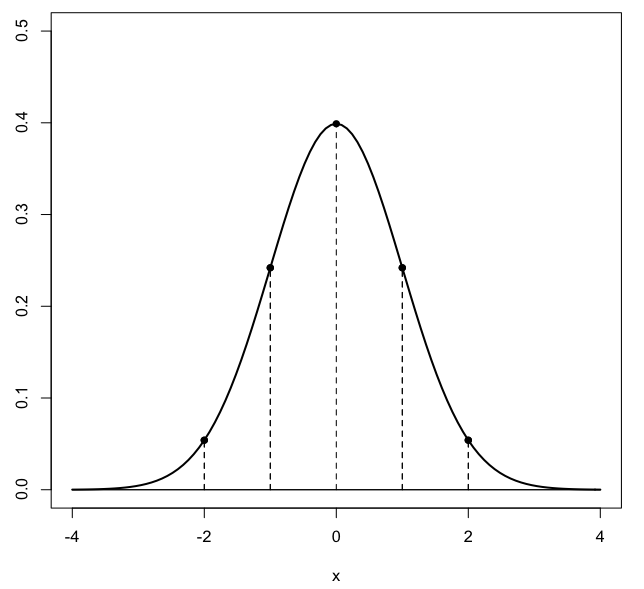
\includegraphics [scale=0.4] {gauss3.png} \end{center}

\begin{document}
\maketitle
%
\tableofcontents

\Large
\chapter{Introduction}
In this short exposition, which has now become a small book, we will analyze a number of problems involving integrals, mainly of geometric figures and solids but a few more just because they are my favorites.

When a sphere is sliced by a plane to form two pieces, we can find the surface areas and volumes of those pieces, and also look at slices lying between two parallel planes, where the surface is called a belt.  

Another problem to solve is called the "cored apple."  Here is a figure that I got from Richard Hamming's \emph{Calculus}.  The central core with light shading has been removed from the sphere and we are interested in what's left.
\begin{center} 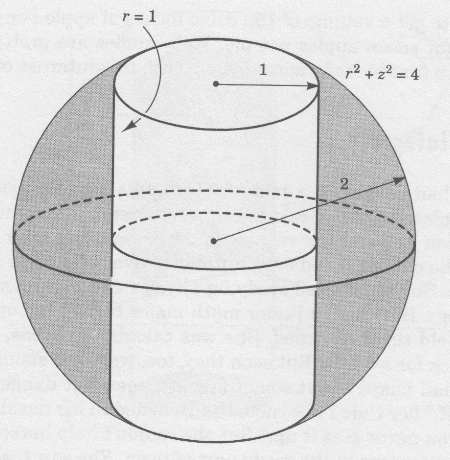
\includegraphics [scale=0.30] {apple_core.png} \end{center}
Simple calculus can be used to solve these, but it is fun to explore geometric proofs as well.   These are some of my favorite topics in mathematics, and I originally called this collection "slicing apples".  Near the end, we will deal with some fairly sophisticated topics, but we get there gradually.

Let's start with Archimedes.
\chapter{Archimedes}
\section*{sphere:  volume}
\subsection*{geometry}
The very first derivation of the volume of a sphere was discovered by Archimedes.
The following is a simple argument (supposedly slightly different than the one he actually used).  

We compare a half-sphere and an inverted cone to a cylinder.  
\begin{center} 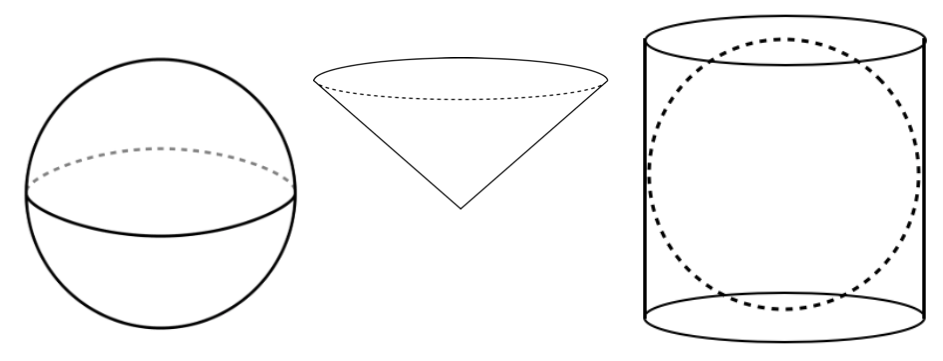
\includegraphics [scale=0.4] {scc1.png} \end{center}

Below is a diagram showing a vertical cross-section through the center of each solid so we can visualize the geometry.  The radius $R$ is the same for all three.  In addition, the cone has overall height equal to $R$.
\begin{center} 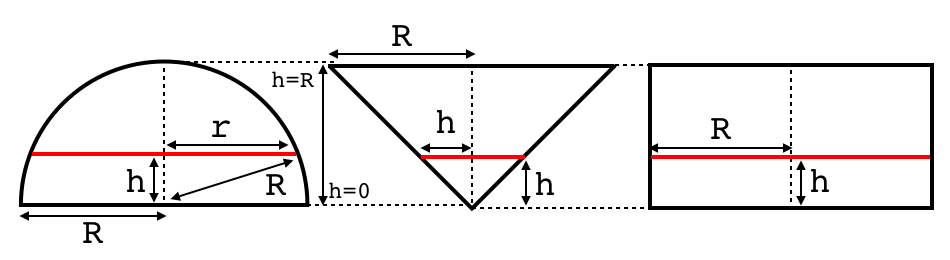
\includegraphics [scale=0.45] {scc2.png} \end{center}

Now we imagine making a horizontal slice through each solid at the height $h$, shown by the red lines.  We will choose different values of $h$ later and compare the results, the one shown here is arbitrary.

If you visualize this you should be able to see that each of these red slices is actually a circle in three-dimensional space.  The question we ask is:  

\textbf{what is the area for each horizontal slice}?

We need to determine the radius for each red circle.  Moving right-to-left, the radius of the cylinder is just $R$.  For the cone, the radius at each height $h$ is equal to $h$ (by similar triangles).  And for the sphere, we use the Pythagorean theorem to find that
\[ r^2 + h^2 = R^2 \]
\[ r^2 = R^2 - h^2 \]

The first insight of the proof is to recognize that the radius squared for the sphere's slice ($r^2$), plus the radius squared for the cone ($h^2$) is equal to $R^2$, the radius squared for the cylinder.  

And since the areas are proportional to $r^2$ (namely $A = \pi r^2$ for these circles), the areas add too:  \textbf{sphere plus cone equals cylinder}.

The second insight of the proof is to recognize that this property does not depend on the height at which we make the slice.  The three slices obtained at any height $h$ add up like this.  So if we imagine making a bunch of slices for each solid and adding them all up to find the volume, the volumes will add too.

The volume of the cylinder is simply $\pi R^3$.  The volume of the cone is known to be one-third the area of the base times the height, or $1/3 \ \pi R^3$.  (See below for a derivation).

We subtract to find that the area of the half-sphere is $2/3 \ \pi R^3$, and therefore the volume of the whole sphere is
\[ V_{\text{sphere}} = \frac{4}{3} \pi R^3 \]

There is a bit of a trick here to hide the idea introduced in calculus, which makes this thinking rigorous.  The sphere and cone have variable widths, which means that the radius will be different on the top of a slice compared to the bottom.  Therefore, the slices have to be made very thin.  In calculus they become infinitely thin, and then we add up infinitely many of them.

\chapter{Circle and cone}
\section*{Circle:  area}
\subsection*{geometry}
There is an area in geometry that comes before the volume of the sphere, but I held off so as to start with Archimedes.  We want the area of a circle, and we imagine dividing a circle into wedges, like you might do with a pizza.  Here, the pie has been divided into 16 parts.
\begin{center}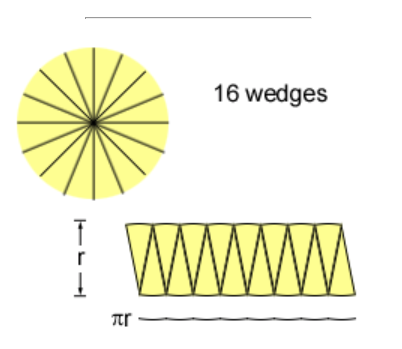
\includegraphics [scale=0.5] {circle_wedges.png}\end{center}

Since the pieces are triangular, it is easy to stack them next to each other with the bases and tips alternating, as shown.  Of course the bases are not straight, but have the same curvature as the edge of the circle.  The length of the short side is $R$, and the length of the long side is approximately one-half the circumference so
\[ A = \frac{1}{2} \cdot 2 \pi R \cdot R = \pi R^2 \]

The trick is to imagine that we subdivide the circle into many slices.  If there are infinitely many  slices, the edges are straight and this calculation becomes exact.

\section*{Cone:  volume}
\subsection*{geometry}
We needed the formula for the volume of a cone above.

Consider a solid cube, with sides of length $s$. Label the central point inside the solid as $P$.  Draw lines connecting each of the 8 external vertices to $P$, something like this. 

\begin{center}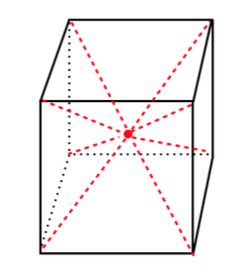
\includegraphics [scale=0.5] {cube_to_cone.png}\end{center}

Now slice the cube on planes that connect all the lines.  (You can't do this easily in real life by slicing up a single cube, because the cuts to form one surface would ruin some of the other pieces).

The result would be 6 identical pieces (square pyramids) looking like this
\begin{center}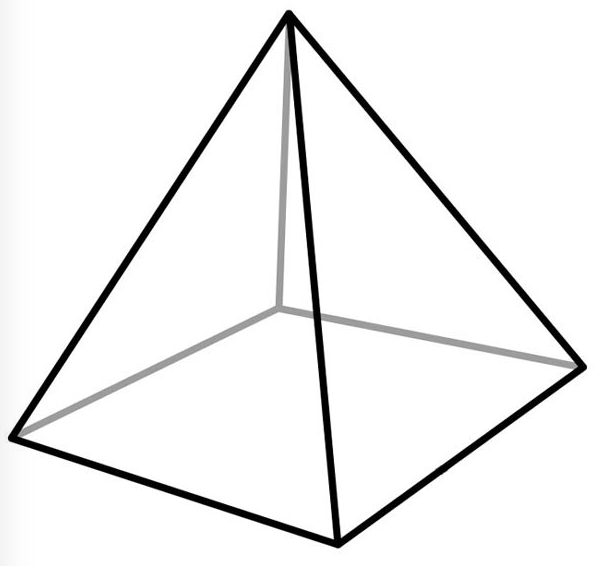
\includegraphics [scale=0.25] {squarepyramid.png}\end{center}

If we started with a cube, the height of the pyramids would $s/2$ (half the side length).  The pyramid in this figure looks to be about twice that.

Let the pyramid volumes be $V$, so 6 of those are equal to the volume that we started with.  We have that
\[ 6V = s^3 \]
\[ V = \frac{1}{3} s^3 \]
Now, we expect that the volume depends linearly on the height and the area of the base, so the more general formula for a pyramid is really a linear function of $h$
\[ V = \frac{1}{3} hs^2 \]
and you can show this by starting with solids that are not cubes but longer in one-dimension.  If that length is $2s$ then the resulting pyramids have heights $h$ and the volume is as shown above.

Of course, a pyramid is not a cone.  But you can use an argument identical to the one we used for the sphere to show that the volume is independent of the shape of the base.  It just depends on the area.  So for a cone we finally obtain
\[ V =  \frac{1}{3} \pi r^2 h \]

Later on we will see several methods for finding this result using calculus.

\chapter{Calculus, gently}
\section*{Circle:  area}
\subsection*{calculus}
Let's spend some time analyzing the area of a circle using calculus.  This provides crucial insight into what integral calculus does.

\begin{center}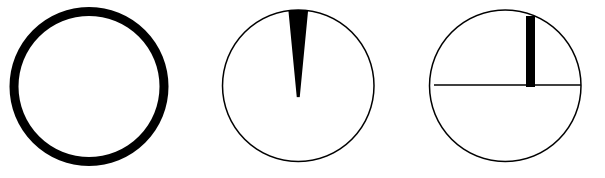
\includegraphics [scale=0.5] {circles.png}\end{center}

Integration is used to compute areas and volumes, and other sums, by adding up many little pieces.  To calculate the area of a circle, we find the pieces we will use with one of three basic strategies:  rings, slices of pie, or rectangles of area underneath the function obtained by solving $x^2 + y^2 = R^2$ (using the positive square root).  These three approaches are illustrated in the figure above.

\subsection*{rings}

In the first approach (left panel), we imagine the area being computed by adding up the individual areas of a series of very thin, concentric rings.

The total area to be computed is that of a circle of a definite, fixed size, and we denote the radius of this circle by capital $R$, a constant.  On the other hand, the series of rings ranges from the origin of the circle to the circumference of the outmost ring.  Each one of this progression of rings has a radius, so we use the lowercase $r$ to describe them, with $r$ being a variable---$r$ varies from $0$ at the origin to $R$ at the outside of the circle.

Think about an individual ring, for example the outermost ring, which is similar to the circular peel or rind surrounding a thin slice of lemon.  We are working with areas here, in two dimensions, so the slice we imagine to be infinitely thin, and we are working with it as a cross-section or ring.

The area of the ring is the length times the width.  The length is the circumference, $2 \pi R$ for the outermost ring, but in general, for any of the inner rings it is $2 \pi r$. The length is multiplied by the width of the slice, which is a small element of radius, $dr$.  The small element of area contributed by an individual ring is $dA$:

\[ dA = 2 \pi r \ dr \]

Another way to explain this equation is to ask the question:

\textbf{how does area change with increasing radius}?  

If we take a circle and increase its radius by a little bit, how does the area change?  The answer is, it changes in proportion to the circumference, $2 \pi r$.

Another way to say the same thing is that the derivative is
\[ \frac{dA}{dr} = 2 \pi r \]

Proceeding from the first equation, the total area is the sum of the areas for the series of rings.

\[ A = \int dA = \int_0^R 2 \pi r \ dr \]

It's worth emphasizing how this view is different than the examples of integration one usually sees first in a calculus book:  these pieces of area are not rectangles but circles.  But it poses most clearly the question we are trying to answer, "how does area vary with $r$"?

The solution is
\[ \int_0^R 2 \pi r \ dr = 2 \pi \ \frac{1}{2}r^2 \ \bigg|_{r=0}^{r=R} = \pi R^2\]
as expected.  And we can check by differentiating:
\[ \frac{d}{dr} \ \pi R^2 = 2 \pi R \]

\subsection*{wedges}

In the second method, we need to first find the area of a wedge.  For a thin enough slice, this is a triangle, with a similar formula: one-half the base times the height.  The height is $R$, the radius of the circle.  

For the base we need the length of a piece of arc of a circle.  Recall that by definition, if we have a unit circle, then the angle of a wedge is equal to the arc it cuts out, and vice-versa, the arc is equal to the angle.  (Thus, the total length if we go all the way around the unit circle is $2 \pi$).  

For a circle with radius $R$, the length going all the way around is $2 \pi R$, and the length of arc for any angle $\theta$ is $\theta$ times $R$.

The area we want is built up of a series of wedges that are almost infinitely slender, with angle $d \theta$, so these wedges have bases measuring $R \ d \theta$.  The area of each triangular wedge is one-half the height times the base or
\[ dA = \frac{1}{2} R \ R \ d\theta \]

For the total area
\[ A = \int dA = \int  \frac{1}{2} R \ R \ d\theta \]
\[= \frac{1}{2} R^2 \int_{\theta=0}^{\theta=2\pi} \ d\theta \]
\[ = \frac{1}{2} R^2 \theta \  \bigg|_{\theta=0}^{\theta=2\pi} \]
\[ =  \pi R^2 \]

\subsection*{area under the curve}
The third view is the most familiar, but has a somewhat harder calculation (some of which we will avoid by a trick).  We need to find the area under the positive square root in the equation for a circle (right panel).
\begin{center}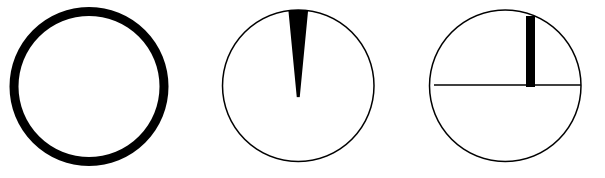
\includegraphics [scale=0.5] {circles.png}\end{center}
\begin{center}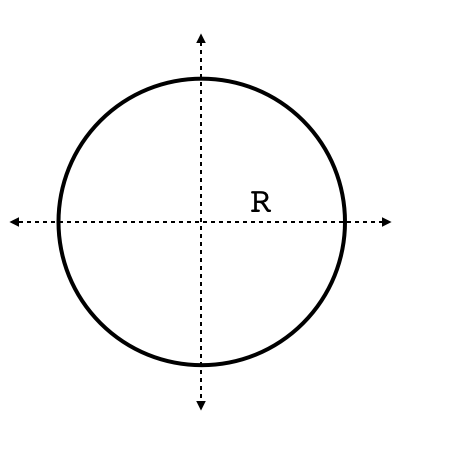
\includegraphics [scale=0.25] {circle.png}\end{center}
\[ x^2 + y^2 = R^2\]
\[ y = f(x) = \sqrt{R^2-x^2} \] 
so we could try to integrate:
\[ \int f(x) \ dx = \int_{-R}^{R} \sqrt{R^2-x^2} \ dx \]
but we don't have $x$ on top of that square root.  We use a trigonometric substitution
\[ x = R \sin t \]
\[ y = R \cos t \]
and
\[ dx = R \cos t \ dt \]
Going back to 
\[ \int y \ dx = R^2 \int \cos^2 t \ d t \]
Leave the factor of $R^2$ aside until the end.

Now for my trick.  I encourage you to try differentiating products of different functions, just to see if you can find interesting integrals.  Suppose we try
\[ \frac{d}{dt} \ \sin t \cos t  = \sin t (- \sin t) + \cos t \cos t \]
\[ = -\sin^2 t + \cos^2 t \]
Using a rearranged standard identity ($-\sin^2 t = \cos^2 t - 1$) we substitute to get
\[ \frac{d}{dt} \ \sin t \cos t  =  (\cos^2 t - 1) + \cos^2 t \]
So
\[ 2 \cos^2 t = 1 + \frac{d}{dt} \ \sin t \cos t \]
\[ \int \cos^2 t = \frac{1}{2} \ [ \ t + \sin t \cos t \ ] \]
We substituted
\[ x = R \sin t \]
so to figure the bounds on $t$, we say that $x = \pm R$ 
\[ \sin t = \pm 1 \]
and thus $t = \pm \ \pi/2$ and we have
\[ \frac{1}{2} \ [ \ t + \sin t \cos t \ ] \bigg |_{-\pi/2}^{\pi/2} \]
The second term is zero because $\cos \pm \ \pi/2 = 0$ and we are left with $\pi/2$.  Pick up the factor of $R^2$, and be sure to look at the diagram and realize that we only computed the half-circle for this part, so the final answer is multiplied by 2.

\chapter{More from Archimedes}
As long as we are talking about areas in the plane, and Archimedes, we should talk about parabolas.

Here is a figure from wikipedia, showing a parabola and a chord of the parabola, which might be drawn between any two points.  A triangle is constructed from the chord in the following way:  the point dividing the horizontal distance in half is found and that is used for the x-value of the third point.

\begin{center} 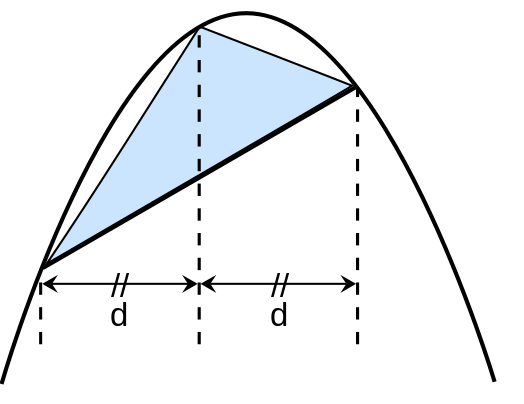
\includegraphics [scale=0.4] {para_tri.png} \end{center}
The Greek genius Archimedes showed that the total area underneath the curve, between the two outside vertices of the triangle, is $4/3$ times the area of the triangle shown in blue. The method he used is called the "quadrature of the parabola" and it is (from our modern perspective) a relatively simple though still revolutionary idea.

One simple and very interesting consequence is that the slope of the tangent to the parabola at this midway point is equal to the slope of the chord.

The general equation of a parabola is
\[ y = ax^2 + bx + c \]
But for any given parabola, we can translate it to the origin and the parabola at the origin with the same shape is
\[ y = ax^2 \]
(where $a>0$).

This can be demonstrated by completing the square.
\[ y = ax^2 + bx + c \]
\[ y - c = ax^2 + bx \]
\[ \frac{y-c}{a} = x^2 + \frac{b}{a} x \]
\[ \frac{y-c}{a} + + \frac{b}{4a^2} = x^2 + \frac{b}{a} x + \frac{b}{4a^2} \]
\[ = (x + \frac{b}{2a})^2 \]
\[ y - c  \frac{b}{4a} = a(x + \frac{b}{4a^2})^2 \]
All the terms except $a$ simply move the vertex.  $a$ is the shape parameter.

If we pick two points on the parabola at $x=u$ and $x=v$, then the corresponding coordinates are
\[ P = (u, \ au^2) \]
\[ Q = (v, \ av^2) \]
\begin{center} 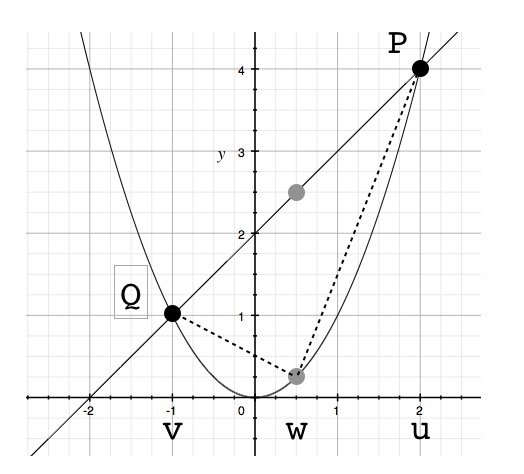
\includegraphics [scale=0.6] {para_tri2.png} \end{center}
$P$ is the right-hand point in the figure.  Let us say that $au^2 > av^2$ and  
and the slope $m$ of the chord that connects them is
\[ m =\frac{au^2 - av^2}{u - v} = \frac{a(u^2-v^2)}{u - v} = \frac{a(u-v)(u+v)}{u - v} \]
so
\[ m = a(u+v) \]
We can see that this formula gives the correct answer for $u = - v$, since the slope at the vertex is $0$.  Now label the midpoint $x=w$
\[ w = \frac{1}{2}(u + v) \]
And the slope at $w$ (from calculus) is
\[ f'(w) = 2aw = = 2a \ \frac{1}{2}(u+v) = a(u + v) \]
So the proposition is correct.

\subsection*{Quadrature}
Another interesting thing about this figure is that the area of the triangle can be found from the length of the vertical coming down from the top that stays inside the blue region.
\begin{center} 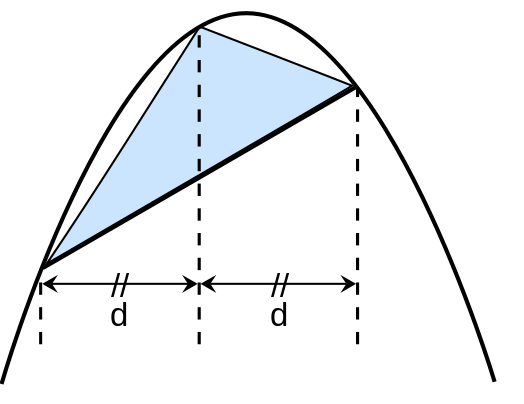
\includegraphics [scale=0.4] {para_tri.png} \end{center}
If we simply turn the graph sideways in our mind, then the two small triangles share this line, which is their "base", $b$.  And they both have "height" $d$, since $w$ was chosen as half way between $u$ and $v$, so their areas are equal, and the total area of the two together is
\[ A = bd \]
We want to find an expression for the area only in terms of $u$ and $v$ (no $b$ or $d$).  Let's look at the second version of the figure again below.  
\newpage
To repeat, what we found above is that the slope at the point on the parabola corresponding to $x=w$ is equal to the slope of the line that connects $v$ and $u$, and more important to us now, that the area of the combined triangle (vertices $u,v,w$) is
\[ A = (u-w) \ b = \frac{1}{2} (u-v) \ b \]
where $b$ is the distance parallel to the $y$-axis between the two points marked in gray.  
\begin{center} 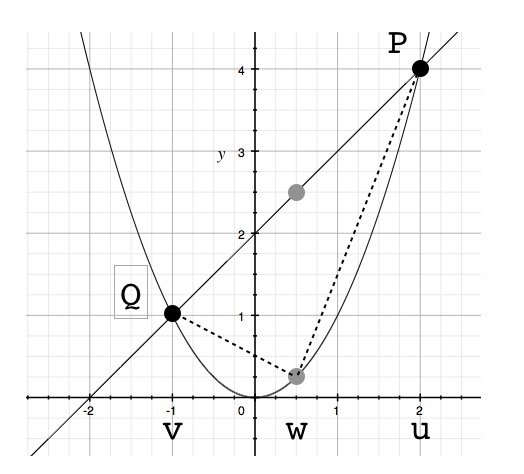
\includegraphics [scale=0.6] {para_tri2.png} \end{center}
The length of the "base" $b$ is the average of the y-values for $x=u$ and $x=v$, minus $aw^2$.
\[ b = \frac{1}{2}(au^2+av^2) - aw^2 \]
and from before
\[ w = \frac{1}{2}(u+v) \]
so we have
\[ b = \frac{1}{2}(au^2+av^2) - a\ [\ \frac{1}{2}(u+v)\ ]^2 \]
Factor out $a/4$
\[ = \frac{1}{4} a\ [\ 2u^2 + 2v^2 - (u+v)^2 \ ] \ \]
\[ = \frac{1}{4} a\ [\ 2u^2 + 2v^2 - u^2 - 2uv - v^2 \ ] \ \]
\[ = \frac{1}{4} a\ [\ u^2 - 2uv + v^2 \ ] \  \]
\[ b = \frac{1}{4} a\ (u-v)^2 \]
The area is
\begin{equation}
\boxed{A = bd = \frac{1}{8} a\  (u-v)^3}
\end{equation}

\subsection*{check}
We'll check three cases to see if this makes sense.  First if 
\[ u = v \]
then the area is zero and $w=u=v$, so that's good.  Second, if 
\[ u = -v \]
then
\[ A = \frac{1}{8} a\ (u-v)^3  = \frac{1}{8} a\  (2u)^3  = au^3 \]
We compare this result with a direct computation by geometry.  In the figure we have two symmetric triangles with individual area 
\[ \frac{1}{2} u \ au^2 \]
The total area is twice that, so it checks.  Finally, suppose we have $v = 0$
\[ A = \frac{1}{8} a\  (u-v)^3 \]
This one is harder to see, but we have that 
\[ d = \frac{1}{2} (u-v) = \frac{1}{2}u \]
$b$ is the distance between the average y-value which is $(1/2)au^2$ and $aw^2 = a(u/2)^2$
\[ b = a\   (\frac{1}{2}u)^2 - \frac{1}{2}\ [\ au^2-0\ ]\  = \ \frac{1}{4}a \ u^2 \]
\[ A = bd = \frac{1}{8}au^3 \]
so they all check.

\subsection*{Quadrature of the parabola}
\begin{center} 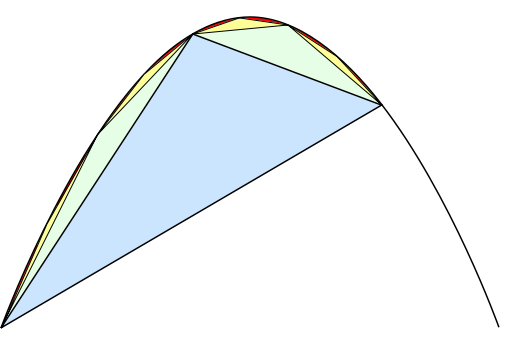
\includegraphics [scale=0.6] {para_tri3.png} \end{center}
The reason for the whole preceding argument is this.  The area formula is
\[ A = bd = \frac{1}{8} a\ (u-v)^3 = k(u-v)^3, \ \ k = const \]
It is solely a function of $u-v$.  Suppose we draw two new triangles (in light green, above).  For each of these triangles the distance between the new vertices is one-half what we had before.  So everything that we have for the big blue triangle is also true for these two new ones, just adjusted by a factor of $u'-v' = (1/2)(u-v$).

What this means is that the area of each light green triangle is in the ratio to the blue one of $(1/2)^3 = 8$.  But there are two of these new triangles, so the new area we added is in the ratio $1/4$.

Suppose we do it again, constructing the yellow triangles.  The new area of each is in the ratio $(1/4)^3 = 1/64$ but there are now $4$ of these yellow triangles so the total area is in the ratio $1/16 = (1/4)^2$

If we call the area of the original triangle $T$, that of the blue plus the light green is

\[ A = T + \frac{1}{4} T \]
and with the addition of the yellow it is

\[ A = T + \frac{1}{4} T  + \frac{1}{16} T \]
so, as an infinite series it is

\[ A = T(1 + \frac{1}{4} + \frac{1}{16} + \cdots ) \]

Here is Archimedes' proof that the sum of this series (not counting the first term) is $1/3$.  

\begin{center} 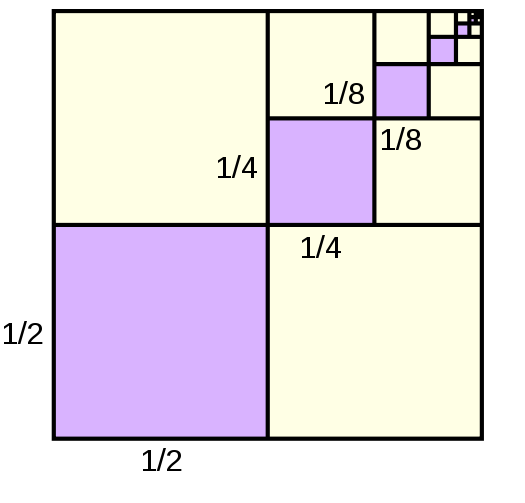
\includegraphics [scale=0.4] {para_series_sum.png} \end{center}
So the total is $4/3$, and the complete area under the parabola is $4/3$ the area of the triangle drawn as we described!

This called the "method of exhaustion."

\chapter{Sphere and Cone}
\section*{sphere:  volume}
\subsection*{calculus (1 variable)}
Draw a circle of radius $R$, centered at the origin.
\begin{center} 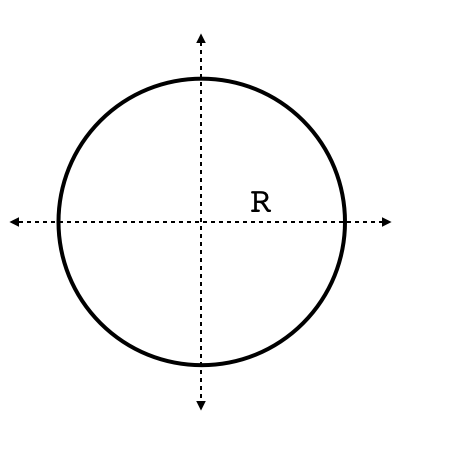
\includegraphics [scale=0.45] {circle.png} \end{center}
Points on the circle obey the standard equation
\[ x^2 + y^2 = R^2 \]
Rearrange and take the square root to get $y$ as a function of $x$
\[ y = f(x) = \sqrt{R^2 - x^2} \]
For this \emph{function}, we would emphasize that we must choose one root, typically the positive one corresponding to the upper half-circle.  Here, though, it doesn't matter, because are really interested in vertical slices through the whole sphere.  These slices have radius $y$ and the area of each slice is $\pi y^2$.

Move from left to right, from $x=-R$ to $x=R$ and add up the areas of all those slices:
\[ V = \int_{-R}^{R} \pi y^2 \ dx \]
\[ = \pi \int_{-R}^{R} (R^2 - x^2) \ dx \]
\[ = \pi(R^2 x - \frac{x^3}{3}) \ \bigg |_{-R}^{R} \]
At the upper bound, the term in parentheses is $2/3 R^3$, and at the lower bound it is $- 2/3 R^3$, so subtracting we obtain 
\[ V = \frac{2}{3} \pi R^3 - (-\frac{2}{3} \pi R^3) = \frac{4}{3} \pi R^3 \]
as expected.

If you find evaluation of the lower bound confusing (as I often do), note that here the integrand is an even function of $x$:
\[ f(x) = f(-x) \] 
and so
\[ \int_{-R}^R f(x) \ dx = 2 \int_{0}^R f(x) \ dx \]
Take the integral from $0$ to $R$ and multiply by two.  At this lower bound the value of the integral is zero.

There are several other derivations that use only one-variable calculus.  My favorite of all is to integrate the surface area as a function of $r$, the radius.  But I would rather work out that result the other way around.  We will talk later about the surface area as the derivative of the volume with respect to $r$.

Another way is to use the theorems of Pappus to find the volume of a "solid of revolution", namely rotation of a half-circle with its base on the $x$-axis, around that same axis.  You can read about it here

\url{http://mathworld.wolfram.com/PappussCentroidTheorem.html}

We will cover this in a later chapter.

\subsection*{shells}

Here is a picture of what we're doing, from \emph{Hamming}.  The notation is different but the idea is the same.

\begin{center} 
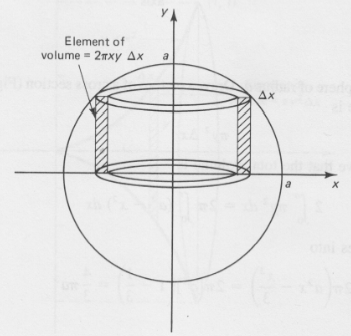
\includegraphics [scale=0.6] {sphere_vol2.png} 
\end{center}

We'll work with the hemisphere, above the $xy$-plane.

Let's divide the sphere up into concentric cylinders or shells, and let $r$ vary from $0 \to R$.  The circumference of the shell at each point is 
\[ C = 2 \pi r \]
and the height of each is 
\[ h = \sqrt{R^2 - r^2} \]
The volume of each very thin cylinder is
\[ dV = Ch \ dr = 2 \pi r \sqrt{R^2 - r^2} \ dr \]
and we want
\[ \int_{0}^{R} 2 \pi r \sqrt{R^2 - r^2} \ dr \]
\[ = -\frac{2}{3}\pi (R^2 - r^2)^{3/2} \bigg|_0^R = -\frac{2}{3}\pi \ [ \ - (R^2)^{3/2} \ ] = \frac{2}{3} \pi R^3 \]

Multiply by two to obtain the total volume.

\section*{cone:  volume}
\subsection*{calculus (disks)}
I don't have a figure for this one, but imagine that we have a cone oriented so that it is symmetric about the $x$-axis, with its vertex at the origin and oriented so that it gets larger as we head to the right.

The equation for the line along the edge of the cone is that the $y$ corresponding to each $x$ is proportional to $x$ with proportionality constant $R/H$.  $y$ is like the radius of the cone and $x$ is like the height.
\[ y = \frac{R}{H} x \]

At each $x$ we slice perpendicular to the $x$-axis obtaining a circle of radius $y$ and area $\pi y^2$.  We sum the areas of all these circles
\[ V = \int_0^H \pi y^2 \ dx \]
\[ = \pi \int_0^H ( \frac{R}{H} x)^2 \ dx \]
\[ = \pi \ \frac{R^2}{H^2} \ [ \frac{x^3}{3} \ ] \ \bigg |_0^H \]
\[ = \frac{1}{3} \pi H R^2 \]

\subsection*{shells}
There is another way to "slice" the figure, which is the method of shells.
\begin{center} 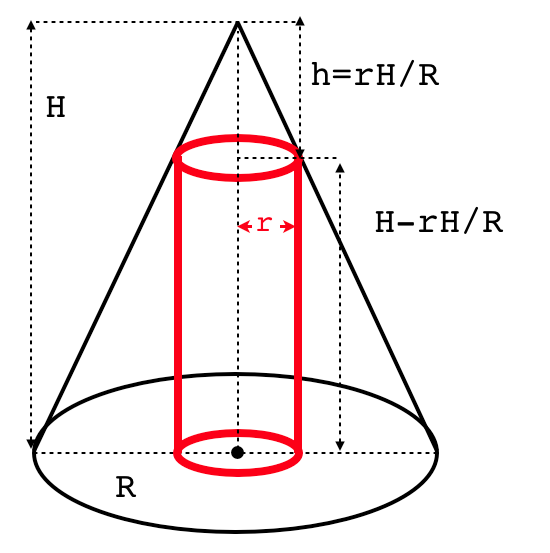
\includegraphics [scale=0.4] {cone_shell2.png} \end{center}
We think of the volume as constructed from a series of concentric cylinders.  Let's use the same letters we had previously, $H$ for total height and $R$ for base radius.  At a height $h$ measured down from the top, the radius $r$ is, as before
\[ r = h\frac{R}{H} \]

Each cylinder has circumference
\[ C = 2\pi r = 2\pi h\frac{R}{H} \]
The height of the cylinder is $H-h$, and the lateral surface area of the shell is
\[ SA = C(H-h) = 2\pi h\frac{R}{H}(H-h) = 2\pi \frac{R}{H} (Hh-h^2)\]
We add up all the shells for $h=0 \to h=H$
\[ V = \int A \ dh = \int_0^H 2\pi \frac{R}{H} (Hh-h^2) \]
\[ = 2\pi \frac{R}{H}(\frac{1}{2}Hh^2 - \frac{1}{3}h^3) \bigg|_0^H = 2\pi \frac{R}{H}(\frac{1}{6}H^3 ) = \frac{1}{3} \pi R^2H \] 

\subsection*{Varying $r$ instead of $h$}
\begin{center} 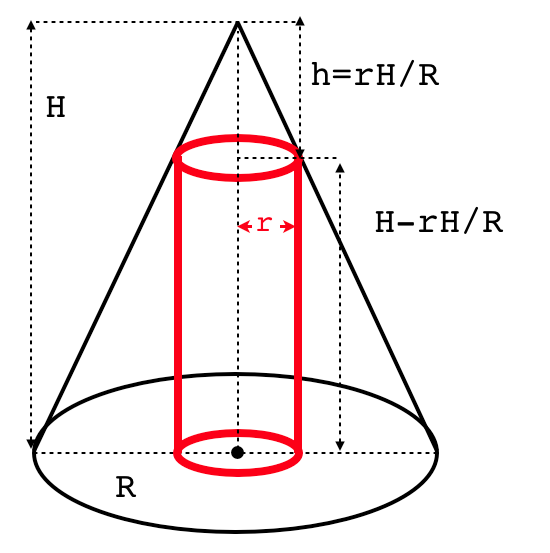
\includegraphics [scale=0.4] {cone_shell2.png} \end{center}
In the previous section we used $h$ as the variable of integration, but we might just as well use $r$.  In that case, $r$ will vary from $r=0 \to r=R$.  At each value, the circumference will be
\[ C = 2 \pi r \]
and the height of the cylinder will be
\[ H-\frac{H}{R}r \]
The volume is the sum of all the little pieces of cylinder volume
\[ V = \int_{r=0}^{r=R} 2 \pi r (H -\frac{H}{R}r) \ dr \]
\[ = 2 \pi H \int_{r=0}^{r=R} r  - \frac{1}{R}r^2 \ dr \]
\[ = 2 \pi H \ (\frac{r^2}{2} - \frac{1}{R}\frac{r^3}{3}) \  \bigg|_0^R \]
\[ = 2 \pi H (\frac{1}{6} R^2) = \frac{1}{3} \pi R^2H \]

\chapter{Double integrals}

Double integrals start with a function of two variables, say $x$ and $y$, $f(x,y)$.  Think of this as a surface with height $z=f(x,y)$, it could be a sloping roof or something more irregular, but still smooth.  Then the integration is performed over a region (an area) in the xy-plane that is the shadow of the surface.  The double integral is the volume contained between the plane and the surface at $z$, within the bounds of the region $R$.
\[ \int \int_R f(x,y) \ dA = ? \]

As our first example, consider the region to be a rectangle with opposing corners at coordinates $(0,0)$ and $(2,1)$.  

\begin{center} 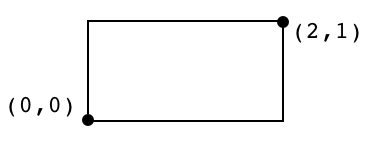
\includegraphics [scale=0.5] {dint1.png} \end{center}

The idea of the integral is that if we slice the volume vertically, say with slices perpendicular to the $x$ axis, we have a standard integral to yield the area of the slice when integrating over $dy$ parallel to the slice, and then in a second integral we add up all of these area slices in the second integral over $x$.  This is known as an \emph{iterated integral}.
\[ \int \int_R f(x,y) \ dA = \int_y \int_x f(x,y) \ dx \ dy = = \int_x \int_y f(x,y) \ dy \ dx = ? \]
Suppose
\[ f(x,y) = xy^2 \]
\[ \int \int_R xy^2 \ dA = ? \]
In this example we sidestep one of the important complications of double integrals compared to single integrals.  Because the area is a rectangle, the bounds of $x$ and $y$ don't depend on where we are in the box, they are the same for each slice.  So, for slices in the vertical direction (integrating over $dy$ first and $dx$ second), we have
\[ \int_{x=0}^{x=2} \int_{y=0}^{y=1} xy^2 \ dy \ dx \]
Here, the \emph{inner} integral is the one we will do first, it is
\[ \int_{y=0}^{y=1} xy^2 \ dy \]
As usual for multivariable calculus, in this computation we treat one variable, here $x$, as a constant.  So we have
\[ \int_{y=0}^{y=1} xy^2 \ dy = \frac{1}{3} xy^3 \ \bigg |_0^1 = \frac{1}{3}x \]
We plug this result into the outer integral
\[ \int_{x=0}^{x=2} \frac{1}{3}x  \ dx = \frac{1}{6} x^2 \ \bigg |_0^2 = \frac{2}{3} \]
Sometimes we will only be able to do a double integral one way, but here we can do it the other way to check
\[ \int_{y=0}^{y=1} \int_{x=0}^{x=2} xy^2 \ dx \ dy \]
Now, the inner integral is 
\[ \int_{x=0}^{x=2} xy^2 \ dx = \frac{1}{2} x^2y^2 \ \bigg |_0^2 = 2y^2 \]
and the outer integral is
\[ \int_{y=0}^{y=1} 2y^2 \ dy = \frac{2}{3}y^3 \ \bigg |_0^1 = \frac{2}{3} \]
They are the same, so that looks good.

Let's do a second example.  Suppose we have the surface $f(x,y) = x^2 + y^2$,  a paraboloid surface opening up.  Our region R is the \emph{Cartesian product} 
\[ R = [-1,1] \times [0,1] \]
We have 
\[ \int \int x^2 + y^2 \ dx \ dy \]
We can do this in either order, so we'll do the inner integral as
\[ \int_{-1}^1 x^2 + y^2 dx = \frac{1}{3}x^3 + xy^2 \ \bigg |_{-1}^{1} = \frac{1}{3} + y^2 - (-\frac{1}{3} - y^2) = \frac{2}{3} + 2y^2 \]
Now the outer integral is
\[ \int_0^1 \frac{2}{3} + 2y^2 \ dy = \frac{2}{3}y + \frac{2}{3}y^3  \ \bigg |_{0}^{1} = \frac{2}{3} + \frac{2}{3} = \frac{4}{3} \]

\subsection*{changed bounds}

\begin{center} 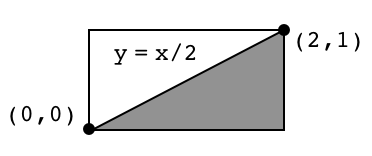
\includegraphics [scale=0.5] {dint2.png} \end{center}

In our second example, we use half of the rectangle, the half that lies below the line $y=x/2$.  Now the upper bound, (the value of $y$) at the top of each slice, is different.

\begin{center} 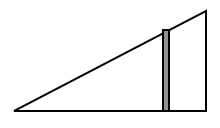
\includegraphics [scale=0.5] {dint3.png} \end{center}

When we integrate $dy$ first, the integral goes from $y=0 \to y=x/2$
\[ \int_{x=0}^{x=2} \int_{y=0}^{y=x/2} xy^2 \ dy \ dx \]
The inner integral is
\[ \int_{y=0}^{y=x/2} xy^2 \ dy = \frac{1}{3} xy^3 \ \bigg |_{y=0}^{y=x/2} = \frac{1}{3}x(\frac{x}{2})^3 = \frac{1}{3} \ \frac{1}{8} \ x^4 \]
and the outer integral is 
\[ \int_{x=0}^{x=2} \frac{1}{3} \ \frac{1}{8}  x^4 \ dx = \frac{1}{3} \ \frac{1}{8}  \frac{x^5}{5} \ \bigg |_{x=0}^{x=2} = = \frac{1}{3} \ \frac{1}{5} \ 4 = \frac{4}{15} \]

On the other hand, if we integrate $dx$ first then the bounds for $x$ are from $x=2y \to x=2$ and $y$ covers the entire range from $y=0 \to 1$. 
\begin{center} 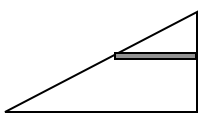
\includegraphics [scale=0.5] {dint4.png} \end{center}

 So we have
\[ \int_{y=0}^{y=1} \int_{x=2y}^{x=2} xy^2 \ dx \ dy \]
The inner integral is
\[ \int_{x=2y}^{x=2} xy^2 \ dy = \frac{1}{2}x^2y^2 \ \bigg |_{x=2y}^{x=2} = 2y^2 - 2y^4 \]
and the outer integral is
\[ \int_{y=0}^{y=1} 2y^2 - 2y^4 \ dy= \frac{2}{3}y^3 - \frac{2}{5}y^5 \ \bigg |_{y=0}^{y=1}  =  \frac{2}{3} - \frac{2}{5} =   \frac{10}{15} - \frac{6}{15} = \frac{4}{15}  \]

\subsection*{Strange limits}
Suppose we do a really simple function with a region whose boundary is something like $y = \ln x$.  We are interested in the region above the curve $y = \ln x$ and below $y=1$.  We go from $x=1$ (where $y=0$) to $x=e$ (where $y=1$).

\begin{center} 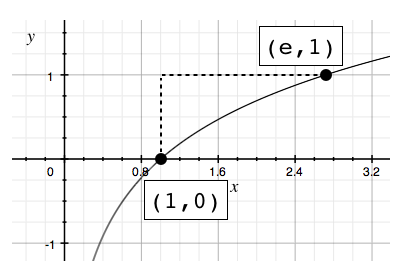
\includegraphics [scale=0.5] {dint5.png} \end{center}

Our simple function is just $1$.  When integrated over the region, this gives the area.
\[ \int \int_R 1 \ dA = A \]
If we integrate $dy$ first, our slices are vertical.  The limits for $y$ are $y = \ln x \to y = 1$.  The limits for $x$ are $x=1 \to x=e$.
\[ \int_{x=1}^{x=e} \int_{y=\ln x}^{y=1} dy \ dx \]
The inner integral is
\[ y  \ \bigg |_{y=\ln x}^{y=1} = 1 - \ln x \]
and the outer integral is
\[ \int_{x=1}^{x=e} 1 - \ln x \ dx =  x - (x \ln x - x) = 2x - x \ \ln x \ \bigg |_{x=1}^{x=e} = 2e - e - 2 + 0 = e - 2 \]

If we do the integral with $dx$ first, we have
\[ \int_{y = 0}^{y=1} \int_{x=1}^{x=e^y} dx \ dy \]
The inner integral is
\[ \int_{x=1}^{x=e^y} dx = x \ \bigg |_{x=1}^{x=e^y} = e^y - 1  \]
and the outer integral is
\[ \int_{y=0}^{y=1}  e^y - 1  \ dy  = e^y - y \ \bigg |_0^1 = e - 1 - 1 + 0 = e - 2 \]

\subsection*{Only one way}
Next, consider
\[ \int \int_R e^{y^2} \ dA \]
We don't have a way to do $dy$ first
\[ \int  e^{y^2} \ dy = ? \]
However
\[ \int  e^{y^2} \ dx = e^{y^2} \ x \]
Now with just the right limits, we might have $x = 0 \to x=y$, then
\[ \int_{x=0}^{x=y}  e^{y^2} \ dx = e^{y^2} \ x \ \bigg |_{x=0}^{x=y} = e^{y^2} \ y \]
We have the $y$ that we need and the outer integral is
\[ \int_{y=0}^{y=1}  e^{y^2} y \ dy = \frac{1}{2} e^{y^2} \ \bigg |_{y=0}^{y=1} = \frac{1}{2}(e-1) \]
\subsection*{Auroux}
In his introduction to double integrals describes the problem of finding the volume under the surface
\[ z = 1 - x^2 - y^2 \]
Visualizing surfaces can be difficult, but here, just set $x=0$ or $y=0$ (separately), then you see that we have a parabola.  This solid is a paraboloid, opening downward, with its apex at $(0,0,1)$.

\begin{center} 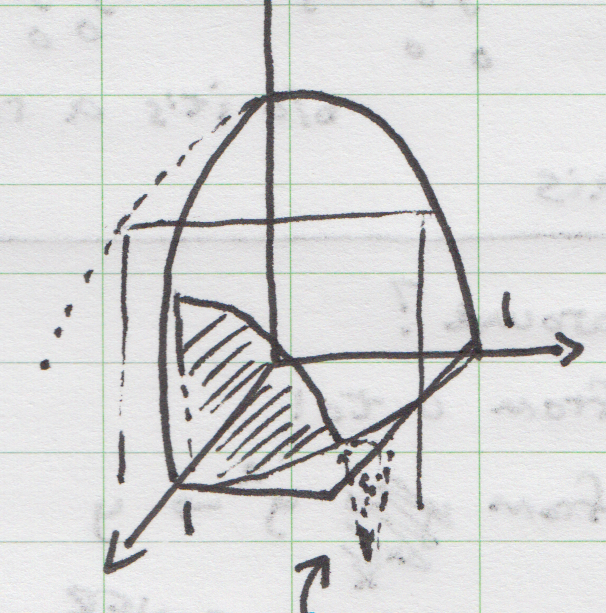
\includegraphics [scale=1.0] {dint.png} \end{center}

The first attempt integrates over the square region $x=0 \rightarrow x=1$ and $y=0 \rightarrow y=1$.  As he points out, this is a bit misguided, because for part of this region, the paraboloid is below the $x,y$-axis.  (If $x=y$ and $z=0$, $x = 1/\sqrt{2}$.  Nevertheless,

\[ \int_0^1 \int_0^1 1 - x^2 - y^2 \ dy \ dx \]
the inner integral is 
\[ y - x^2 y - \frac{1}{3}y^3  \ \bigg |_{0}^{1} = \frac{2}{3} - x^2 \]
and the outer one is
\[  \int_0^1 \frac{2}{3} - x^2 \ dx \]
\[ = \frac{2}{3} x - \frac{1}{3}x^3  \ \bigg |_{0}^{1} = \frac{1}{3} \]

The way to do this problem and actually obtain the volume of the quarter paraboloid is to set up the bounds of integration properly, over the quarter disk.  We can still have $x=0 \rightarrow x=1$ in the outer integral, but for the inner one we use $y=0 \rightarrow y=\sqrt{1-x^2}$.  The changed upper bound makes all the difference.  Now, we have

\[ \int_0^1 \int_0^{\sqrt{1-x^2}} 1 - x^2 - y^2 \ dy \ dx \]
the inner integral is 
\[ (1 - x^2) y - \frac{1}{3}y^3  \ \bigg |_{0}^{\sqrt{1-x^2}} \]
\[= (1-x^2) \sqrt{1-x^2} - \frac{1}{3} (1-x^2)^{3/2} \]
\[ = \frac{2}{3} (1-x^2)^{3/2} \]
Switch to polar coordinates for the outer part

\[ x = \sin \theta \]
\[ dx = \cos \theta \ d \theta \]
\[ \sqrt{1-x^2} = \cos \theta \]
we have
\[ = \frac{2}{3} \int \cos^3 \theta  \cos \theta \ d \theta \]
look it up
\[ = \frac{2}{3} \ [ \ \frac{\cos^3 \theta \ \sin \theta}{3} + \frac{3}{4}( \frac{\theta}{2} + \frac{1}{2} \sin \theta \ \cos \theta ) \ ]  \ \bigg |_{0}^{\pi/2}  \]
At the upper bound, $\cos \pi/2 = 0$ so we get
\[ \frac{2}{3} \ \frac{3}{4} \ \frac{1}{2} \ \frac{\pi}{2} \]
and at the lower bound, $\sin 0 = 0, \theta=0$ so we get $0$.  The result is $\pi/8$.

I would just like to point out another way to find this volume, as a solid of revolution.  Turn the paraboloid and put its apex at the origin, opening to the right.  The equation of its intersection with the $x,y$-plane is just $y=\sqrt{x}$.  For each value of $x=0 \rightarrow x=1$, the cross-section of the paraboloid is a circle of radius $y$ and area $\pi y^2 = \pi x$.  Integrate over the range of $x$

\[ \int_0^1 \pi x \ dx = \pi \frac{1}{2}x^2 = \pi / 2 \]

Recall that we only want $1/4$ of that, or $\pi / 8$.

\subsection*{Two curves}
In Auroux's second example, we have the line $y=x$ and the curve $x=y^2$.  These two curves cross at $(0,0)$ and $(1,1)$, with the line below the curve between these two endpoints.

\begin{center} 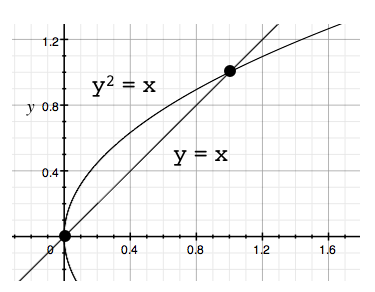
\includegraphics [scale=0.5] {dint6.png} \end{center}

If we integrate $dx$ first, the limits will be $x=y^2 \to x=y$, while if we integrate $dy$ first the limits are $y=x \to y=\sqrt{x}$.

Let's do the area function again ($f(x,y)=1$).
\[ \int \int_R 1 \ dA = ?\]
Start with $dx$ first
\[ \int_{y=0}^{y=1} \int_{x=y^2}^{x=y} \ dx \ dy\]
The inner integral is just
\[ \int_{x=y^2}^{x=y} \ dx  = x  \ \bigg |_{x=y^2}^{x=y} = y - y^2 \]
so the outer integral is
\[ \int_{y=0}^{y=1} y - y^2 \ dy = \frac{1}{2}y^2 - \frac{1}{3}y^3 \ \bigg |_{y=0}^{y=1} =  \frac{1}{2} - \frac{1}{3} = \frac{1}{6} \]
Doing it the other way
\[ \int_{x=0}^{x=1} \int_{y=x}^{y=\sqrt{x}} \ dy \ dx\]
The inner integral is
\[ \int_{y=x}^{y=\sqrt{x}} \ dy  = y  \ \bigg |_{y=x}^{y=\sqrt{x}} = \sqrt{x} - x \]
so the outer integral is
\[ \int_{x=0}^{x=1}\sqrt{x} - x \ dx = \frac{2}{3} x^{3/2} - \frac{1}{2}x^2  \ \bigg |_{x=0}^{x=1} = \frac{2}{3} - \frac{1}{2} = \frac{1}{6} \]

\subsection*{Circle}
Consider a circle of radius $a$ centered at the origin.
\[ x^2 + y^2 = a^2 \]
\[ y = \sqrt{a^2-x^2} \]
This problem is symmetrical so we will only do it one way, integrating over $dy$ first.  
\begin{center} 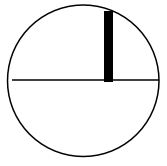
\includegraphics [scale=0.5] {dint7.png} \end{center}

Again, we will do the area function, and we will do only the first quadrant
\[ \int_{x=0}^{x=a}  \int_{y=0}^{y=\sqrt{a^2-x^2}} \ dy \ dx \]
The inner integral is just
\[ \int_{y=0}^{y=\sqrt{a^2-x^2}} \ dy = \sqrt{a^2-x^2} \] 
so now we have for the outer integral
\[ \int_{x=0}^{x=a}  \sqrt{a^2-x^2} \ dx \]
Substitute
\[ x = a \sin \theta, \ \ dx = a \cos \theta \ d \theta \]
For the limits we will have, when $x = 0 \to \theta = 0$ and when $x=a \to \theta=\pi/2$.  (Note that this substitution doesn't match the figure above, so the limits are a bit different.  We used $x=a \sin \theta$).

\[ \int_{x=0}^{x=a}  \sqrt{a^2-x^2} \ dx = \int_{\theta=0}^{\theta=\pi/2} \sqrt{a^2-a^2sin^2\theta} \ a \ cos\ \theta \ d \theta =  a^2 \int_{\theta=0}^{\theta=\pi/2} cos^2\theta \ d \theta \]
\[ = \frac{a^2}{2} \ [ \theta + \sin \ \theta \cos \ \theta \ ] \ \bigg |_{\theta=0}^{\theta=\pi/2} = \frac{a^2}{2} \frac{\pi}{2} =  \frac{\pi}{4} a^2 \] 

\subsection*{Paul}
Here are a couple of examples from Paul's online notes.  

\url{http://tutorial.math.lamar.edu}

The first one is over the region defined by 
\[ R = [-1,2] \times [0,1] \]
What this means is that $x = -1 \to 2$ and y = $0 \to 1$.  The integral is
\[ \int \int_R xe^{xy} \ dA \]
We can see that this will be better to do with $dy$ first.  To make it crystal clear, let's substitute 
\[ u = xy, \ \ du = x \ dy \]
\[ \int xe^{xy} \ dy = \int e^u \ du = e^u = e^{xy} \ \bigg |_0^1 =  e^x - 1 \]
and the outer integral is
\[ \int_{-1}^2 e^x - 1 \ dx = e^x - x  \ \bigg |_{-1}^2 = e^2 - 2 - e^{-1} + 1 = e^2 - e^{-1} - 1 \]

In the next one, we are given the integral already set up
\[ \int_{x=0}^{x=3} \int_{y=x^2}^{y=9} x^3 e^{y^3} \ dy \ dx \]
And of course the problem is that we can't do it this way.  We can do it with $dx$ first, but we need to understand the region that we are integrating over. 

If you draw a sketch, you will see that it is the region above $y=x^2$ and below $y=9$.  We are adding up the slices $f(x,y)$ for $y=x^2 \to y=9$ for every $x = 0 \to 3$.

So our new limits (for slices of the area parallel to the x-axis), we add up $f(x,y)$ for $x=0 \to x=\sqrt{y}$ for every $y = 0 \to 9$.

\[ \int_{0}^9 \int_0^{\sqrt{y}} x^3 e^{y^3} \ dx \ dy \]

So the inner integral is
\[ \int_0^{\sqrt{y}} x^3 e^{y^3} \ dx = \frac{1}{4}x^4 e^{y^3} \ \bigg |_{0}^{\sqrt{y}} = \frac{1}{4}y^2 e^{y^3} \]
Now let 
\[ u = y^3, \ \ du = 3y^2 \ dy, \ \ \frac{1}{3} du = y^2 \ dy \]
and the outer integral is
\[ \int_{0}^9 \frac{1}{4}y^2 e^{y^3} \ dy = \frac{1}{4} \ \frac{1}{3} e^u \ du = \frac{1}{12} e^u = \frac{1}{12} e^{y^3}   \ \bigg |_{0}^9 = \frac{1}{12} (e^{9^3} - 1)\]

Finally, let's recall that in single-variable calculus, to obtain the area between two curves ($g_1(x)$ and $g_2(x)$) for $x = a \to b$ we would integrate the two separately and subtract the lower from the upper.

where the second is always larger than the first $g_2(x) > g_1(x) \ \forall \ x \in [a,b] $.
\[ A = \int_a^b g_2(x) - g_1(x) dx \]

In multi-variable calculus to get the area we integrate

\[ \int \int_R dA \]
over the appropriate bounds.  Here, that leads to
\Large
\[ \int_{x=a}^{x=b} \int_{y=g_1(x)}^{y=g_2(x)} \ dy \ dx = \int_{x=a}^{x=b} g_2(x) - g_1(x) \ dx \]
which is exactly the same thing.

\chapter{Vector dot product}

This chapter introduces a way of multiplying two vectors, the \emph{dot product}, and derives the relationship between the dot product of two vectors and the angle between them.  Suppose we have two vectors
\[ \mathbf{a} = \ \langle a_1,a_2 \rangle \]
\[ \mathbf{b} = \ \langle b_1,b_2 \rangle \]
Geometrically, we might think of these as being one vector extending from the origin in the $x,y$-plane to the point $(a_1,a_2)$, and the other vector extending from the origin to $(b_1,b_2)$.  The dot product is defined as 
\[ \mathbf{a} \cdot \mathbf{b} = a_1 b_1 + a_2 b_2 \]
We can extend this to a pair of vectors in $n$-dimensional space
\[ \mathbf{a} = \ \langle a_1,a_2, \dots a_n \rangle \]
\[ \mathbf{b} = \ \langle b_1,b_2, \dots b_n \rangle \]
\[ \mathbf{a} \cdot \mathbf{b} = a_1 b_1 + a_2 b_2 + \dots + a_n b_n \]
Notice that the two vectors being multiplied (whose dot product is computed) must have the same dimension, the same $n$.  Also, the result of the multiplication---the dot product---is a number.  This is in contrast to another form of vector multiplication (the cross-product) which yields a vector as the result.
\subsection*{Some properties}
The dot product obeys the usual rules:  it is associative, commutative and distributive.  As one example, suppose
\[ \mathbf{b} = \mathbf{c} + \mathbf{d} \]
Then 
\[  \mathbf{a} \cdot \mathbf{b} =  \mathbf{a} \cdot ( \mathbf{c} + \mathbf{d}) = \mathbf{a} \cdot \mathbf{c} + \mathbf{a} \cdot \mathbf{d} \]
You can easily verify this by computing each term of the respective products.
\[ \mathbf{b} = \ \langle b_1,b_2 \rangle \ = \mathbf{c} + \mathbf{d} = \ \langle c_1+d_1,c_2+d_2 \rangle \ \]  
\[  \mathbf{a} \cdot \mathbf{b} = \ \langle a_1(c_1+d_1),a_2(c_2+d_2) \rangle \ \]  
\[ =  \ \langle a_1 c_1+a_1 d_1, a_2 c_2+ a_2 d_2 \rangle \ \]
\[ =  \ \langle a_1 c_1,a_2 c_2> \ + \ \langle a_1 d_1 , a_2 d_2 \rangle \ \]
\[ = \mathbf{a} \cdot \mathbf{c} + \mathbf{a} \cdot \mathbf{d} \]
A second example that we will need below is
\[ ( \mathbf{a} -  \mathbf{b}) \cdot ( \mathbf{a} -  \mathbf{b}) =  \mathbf{a} \cdot \mathbf{a} -  \mathbf{a} \cdot \mathbf{b} -  \mathbf{b} \cdot \mathbf{a} +  \mathbf{b} \cdot \mathbf{b}   \]
Since $\mathbf{a} \cdot \mathbf{b}  = \mathbf{b} \cdot \mathbf{a}$ we have
\[ ( \mathbf{a} -  \mathbf{b}) \cdot ( \mathbf{a} -  \mathbf{b}) =  \mathbf{a} \cdot \mathbf{a} +  \mathbf{b} \cdot \mathbf{b}  - 2 \ \mathbf{a} \cdot \mathbf{b}  \]

\subsection*{Length of a vector}
Recall that the length of a vector $\mathbf{a} = \ \langle a_1,a_2 \rangle $, designated $|\mathbf{a}|$, is computed by a straightforward application of the Pythagorean Theorem:
\[ |\mathbf{a}|^2 = a_1^2 + a_2^2 \]
We leave the result as the square for simplicity.  This is easily extended to more dimensions by sequential application of the same method.  In $\mathbb{R}^3$:
\[ |\mathbf{a}|^2 = a_1^2 + a_2^2 + a_3^2 \]
In $\mathbb{R}^n$:
\[ |\mathbf{a}|^2 = a_1^2 + a_2^2 + \dots + a_n^2 \]
Notice that
\[ |\mathbf{a}|^2 = \mathbf{a} \cdot \mathbf{a} \]

\subsection*{Relation to $\theta$}
Now we are ready for the main idea.  Suppose we draw two vectors $\mathbf{a}$ and $\mathbf{b}$ in $\mathbb{R}^2$ with their tails at the same point.  Designate the angle between them as $\theta$ and the vector representing the side opposite as $\mathbf{c}$.  
\begin{center} 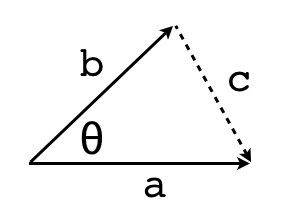
\includegraphics [scale=0.4] {dot1.png} \end{center}
The orientation of  $\mathbf{c}$ doesn't matter for the argument that follows.  As shown
\[ \mathbf{b} + \mathbf{c} = \mathbf{a} \]
\[ \mathbf{c} = \mathbf{a} - \mathbf{b} \]
Compute the dot product of $\mathbf{c}$ with itself
\[ \mathbf{c} \cdot \mathbf{c} = ( \mathbf{a} -  \mathbf{b}) \cdot ( \mathbf{a} -  \mathbf{b}) \]
Recalling the result from above, this is
\[ \mathbf{c} \cdot \mathbf{c} = \mathbf{a} \cdot \mathbf{a} +  \mathbf{b} \cdot \mathbf{b}  - 2 \ \mathbf{a} \cdot \mathbf{b}  \]
Since 
\[ |\mathbf{a}|^2 = \mathbf{a} \cdot \mathbf{a} \]
and so on, we have that
\[ \mathbf{c} \cdot \mathbf{c} =  \mathbf{a} \cdot \mathbf{a} +  \mathbf{b} \cdot \mathbf{b}  - 2 \ \mathbf{a} \cdot \mathbf{b}  \]
\[ |\mathbf{c}|^2 =  |\mathbf{a}|^2 + |\mathbf{b}|^2  - 2  \ \mathbf{a} \cdot \mathbf{b}  \]
Does this remind you of the \emph{Law of Cosines}?  In ordinary trigonometry, we designate the lengths of a triangle's sides as $a,b,c$ and the angle between sides $a$ and $b$ as $\theta$ and the law says that
\[ c^2 = a^2 + b^2 - 2 a b \cos \theta \]
Comparing the two equations, we see that
\[ \mathbf{a} \cdot \mathbf{b} = |\mathbf{a}| \ |\mathbf{b}| \ \cos \theta \]
This relationship is extremely useful because it allows us to compute the cosine of the included angle via the dot product.  Even more important, two vectors which are perpendicular will have $\cos \theta = 0$, so their dot product is zero.  And although we haven't proved it, this result extends to vectors in $\mathbb{R}^n$.
For example, suppose I have the vector
\[ \mathbf{u} = \ \langle p,q \rangle \]
Find a vector $\mathbf{v}$ perpendicular to $\mathbf{u}$.
\[ \mathbf{v} = \ \langle q,-p \rangle \ \]
$\mathbf{v}$ is perpendicular to $\mathbf{u}$ because
\[ \mathbf{u} \cdot \mathbf{v} = p \times q + (- q) \times p = 0 \]
How to find a vector in $\mathbb{R}^5$ perpendicular to $\langle 1,1,1,1,0 \rangle$?
Any vector of the form $\langle 0,0,0,0,k \rangle $ will do, where k is some real number.
\subsection*{Alternate derivation}
Here is another approach which doesn't depend on knowing the law of cosines, but instead requires the rule for subtraction of cosines
\[ \cos (\theta - \phi) = \cos \theta \cos \phi + \sin \theta \sin \phi \]
Go back to the previous figure
\begin{center} 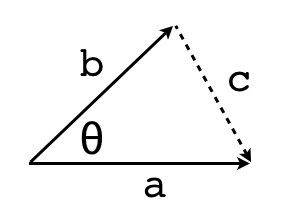
\includegraphics [scale=0.4] {dot1.png} \end{center}
but now imagine that the vector $\mathbf{a}$ forms an angle $\theta_a$ with the $x$-axis and similarly, $\mathbf{b}$ forms an angle $\theta_b$ with the $x$-axis.

If we turn the vector $\mathbf{a}$, then the component of $\mathbf{a}$ that lies along the $x$-axis is $a \cos \theta_a$ (where $a$ is the length of $\mathbf{a}$).  And in a similar vein
\[ a_x = a \cos \theta_a \]
\[ b_x = b \cos \theta_b \]
\[ a_y = a \sin \theta_a \]
\[ b_y = b \sin \theta_b \]
We said that the definition of the dot product is
\[ \mathbf{a} \cdot \mathbf{b} = a_x b_x + a_y b_y \]
\[ = a \cos \theta_a b \cos \theta_b + a \sin \theta_a b \sin \theta_b \]
\[ = ab (\cos \theta_a \cos \theta_b + \sin \theta_a \sin \theta_b) \]
using the subtraction rule this is just
\[ = ab \cos (\theta_a - \theta_b) \]
but since $\theta = \theta_a - \theta_b$
\[ \mathbf{a} \cdot \mathbf{b} = ab \cos \theta \]

\subsection*{Projection}
If $|\mathbf{a}| = 1$ we say that $\mathbf{a}$ is a \emph{unit vector}.  In that case
\[ \mathbf{b} \cdot \mathbf{a} = |\mathbf{b}| \cos \theta \]
Looking at the figure, $|\mathbf{b}| \cos \theta$ is the length of the \emph{projection} of $\mathbf{b}$ on $\mathbf{a}$.  (Recall that the dot product is a scalar---a number---and not a vector).
\begin{center} 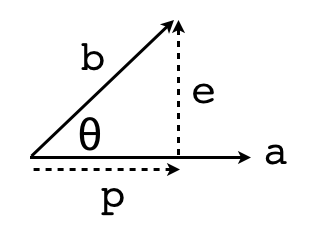
\includegraphics [scale=0.4] {dot3.png} \end{center}
The result, $\mathbf{b} \cdot \mathbf{a} = |\mathbf{b}| \cos \theta$, is the length of the part of $\mathbf{b}$ that extends in the same direction as $\mathbf{a}$.  The corresponding vector is 
\[ \mathbf{p} = (\mathbf{b} \cdot \mathbf{a}) \ \mathbf{a} \]
The other component of $\mathbf{b}$ is the part that is perpendicular to $\mathbf{p}$
\[ \mathbf{p} + \mathbf{e} = \mathbf{b} \]
We compute $\mathbf{e}$ as the difference $\mathbf{b} -  \mathbf{p}$.  $\mathbf{e}$ is the part of $\mathbf{b}$ that is perpendicular to the projection.  As a final note, the formula given here is a simplification for the situation in which $\mathbf{a}$ is a unit vector.  If not, the complete formula is:
\[ \mathbf{p} = \frac{\mathbf{b} \cdot \mathbf{a}}{\mathbf{a} \cdot \mathbf{a}} \ \mathbf{a} \]

\chapter{Vector cross product}

Here, we continue to explore the algebraic manipulation of vectors, including a brief review of the dot product (sometimes called the \emph{inner} product), and a more detailed look at the cross (vector) product.

Define two vectors $\mathbf{a}$ and $\mathbf{b}$:
\[ \mathbf{a} = \ \langle a_1, a_2 \dots \ a_n \rangle \]
\[ \mathbf{b} = \ \langle b_1, b_2 \dots \ b_n \rangle \]

The dot product is the sum of the products of the individual terms
\[ \mathbf{a} \cdot \mathbf{b} = a_1 b_1 + a_2 b_2 + \dots \ a_n b_n \]
\[ = \sum_i a_i b_i \]
The dot product of two vectors is a number, in vector terminology it is called a \emph{scalar}.  The result may be positive, or negative or even zero.

The dot product of a vector with itself is the square of the length or magnitude
\[ \mathbf{a} \cdot \mathbf{a} = a_1 a_1 + a_2 a_2 + \dots \ a_n a_n \]
(this is just the extension of the Pythagorean theorem to three or more dimensions).  

There is another definition of the dot product which can be shown to be equivalent:
\[ \mathbf{a} \cdot \mathbf{b} = |\mathbf{a}| |\mathbf{b}| \cos \theta \]
The dot product is equal to the magnitude of $\mathbf{a}$ times the magnitude of $\mathbf{b}$ times the cosine of the angle between them.  (Note that this definition indicates that the dot product must be independent of the coordinate system).

A proof of this statement about the dot product comes from the law of cosines.  

For a triangle with sides $a$, $b$ and $c$ and angles opposite those sides $A$, $B$ and $C$, divide the third side into two lengths $c=d+e$ using the vertical altitude from vertex $C$.
\begin{center} 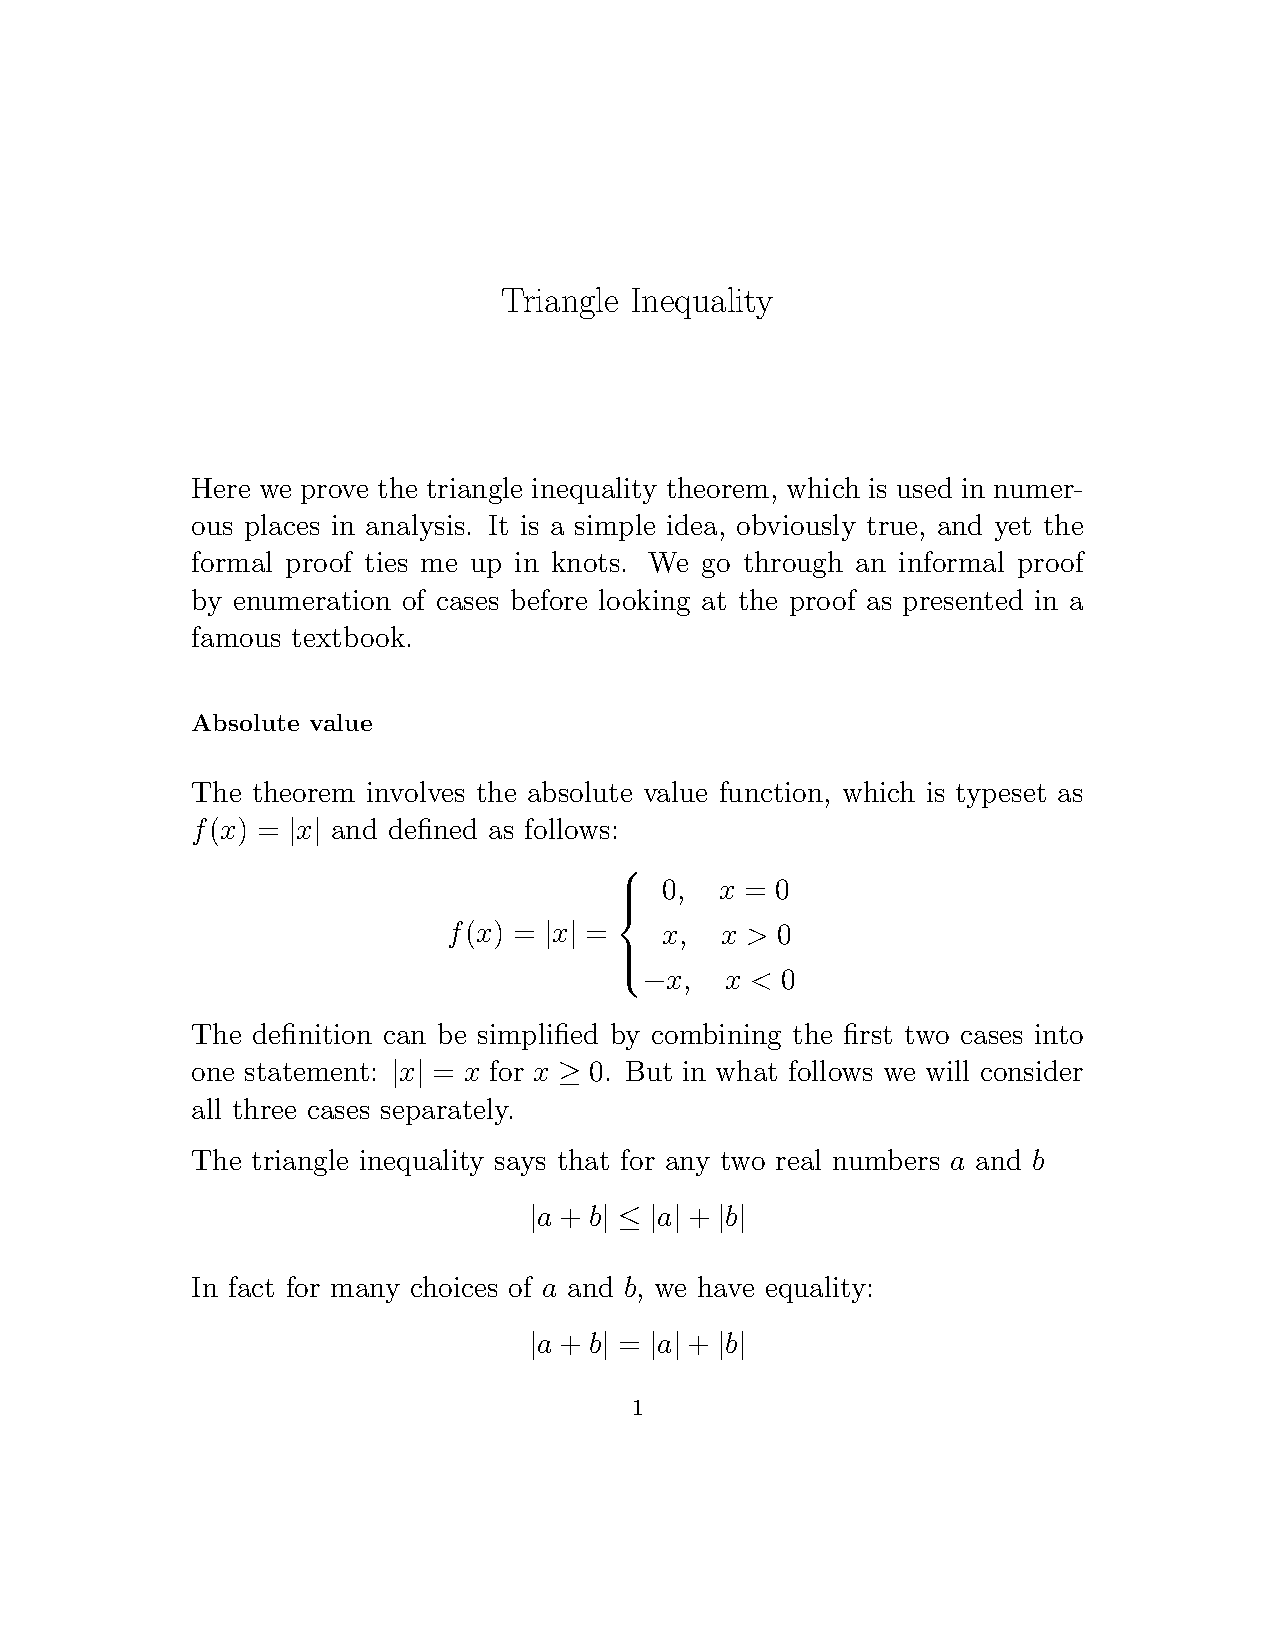
\includegraphics [scale=0.5] {triangle.png} \end{center}
\[ a^2 - e^2 = h^2 = b^2 - d^2 \]
So
\[ a^2 = e^2 + b^2 - d^2 \]
Since $d = c - e$ and thus $d^2 = c^2 - 2ce + e^2$:
\[ a^2 = e^2 + b^2 - (c^2 - 2ce + e^2) \]
\[ = b^2 - c^2 + 2ce  \]
but $e = a \cos B$ so
\[ a^2 = b^2 - c^2 + 2ac \cos B  \]
rearrange to give a more familiar form (this is the law of cosines)
\[ b^2 = a^2 + c^2 - 2ac \cos B  \]
Any side of a triangle can be expressed in terms of the other two and the cosine of the angle between them.  Thus, for example
\[ c^2 = a^2 + b^2 - 2ab \cos C  \]
\[ a^2 = b^2 + c^2 - 2bc \cos A  \]

Now, to compare with the dot product, label side $b$ as the vector $\mathbf{b}$ extending from vertex $A$ to $C$, similarly, label side $c$ as the vector $\mathbf{c}$ extending from vertex $A$ to $B$.  The angle between the two vectors is the angle $A$.
\begin{center} 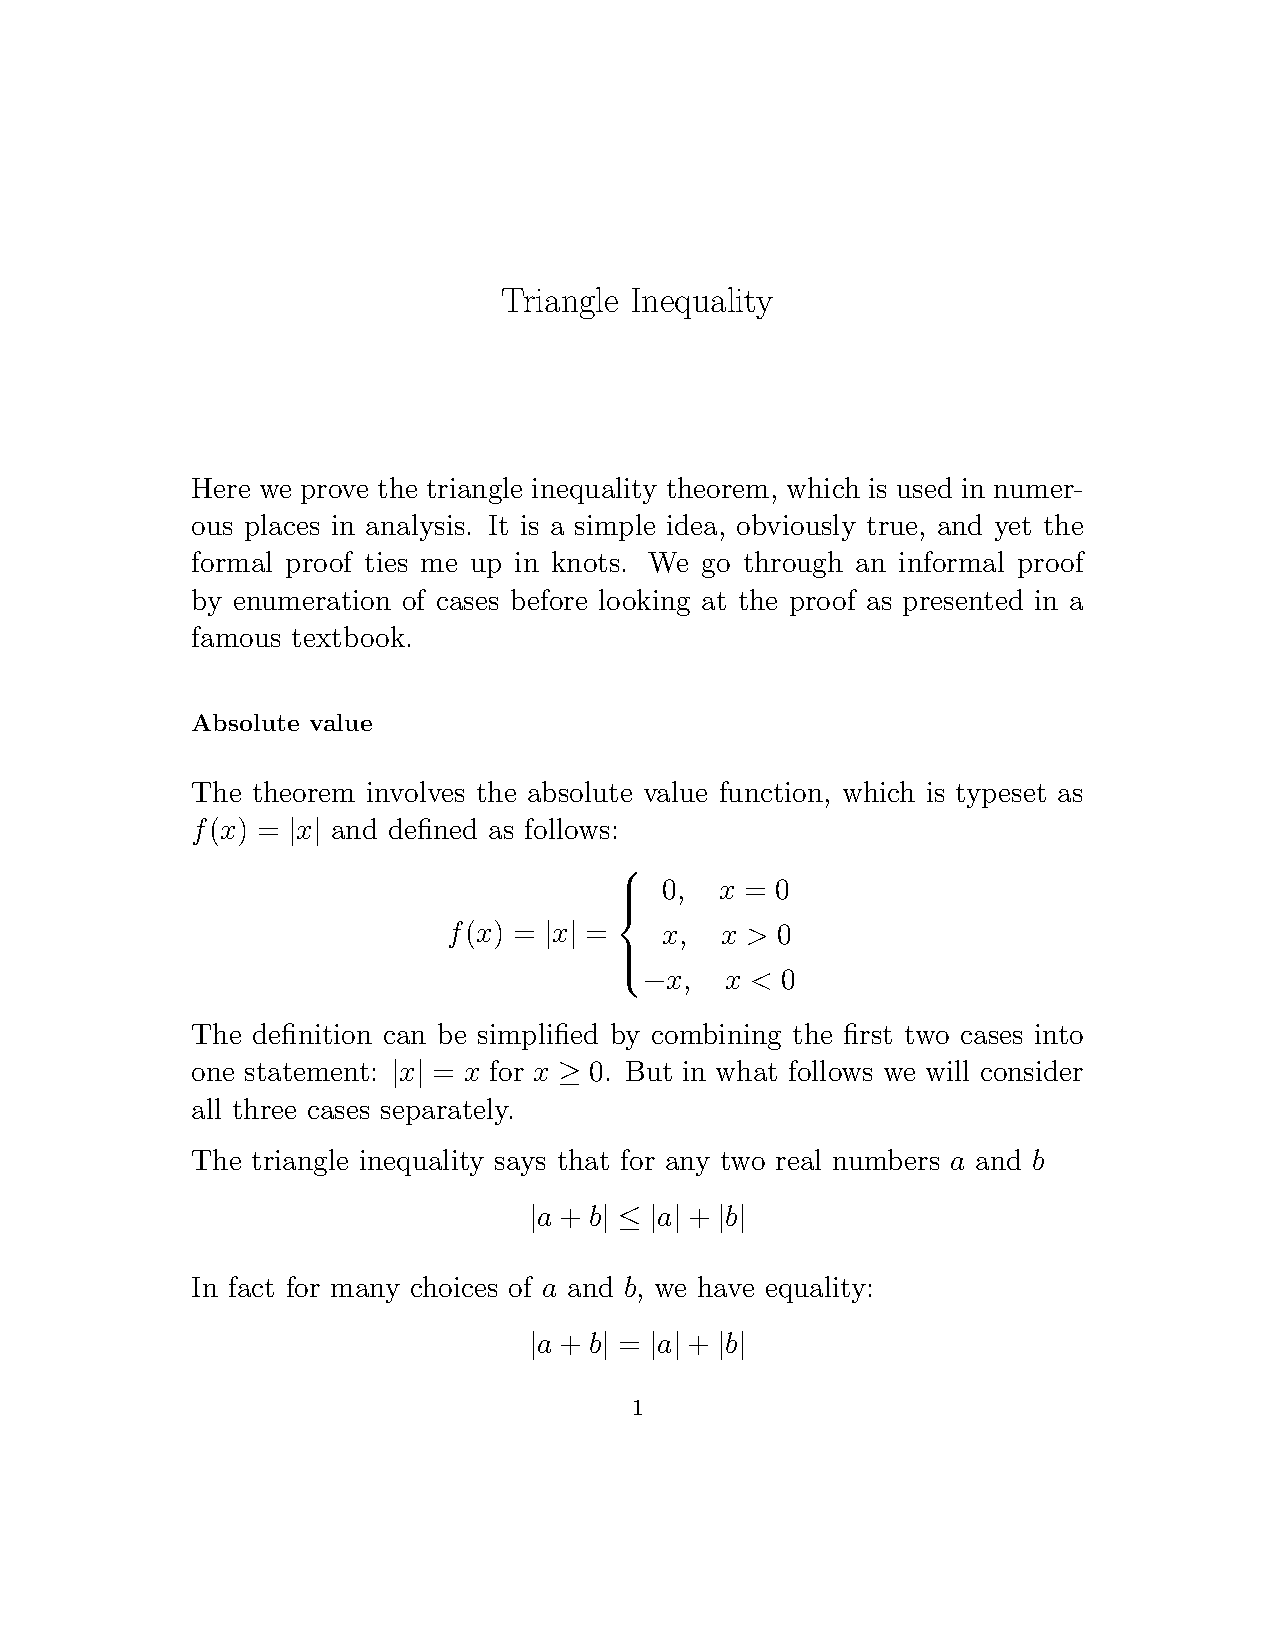
\includegraphics [scale=0.5] {triangle.png} \end{center}
If we view side $a$ as the vector $\mathbf{a}$, extending from vertex $C$ to $B$, then
\[ \mathbf{b} + \mathbf{a} = \mathbf{c} \]
\[ \mathbf{a} = \mathbf{c} - \mathbf{b} \]
The length of side $a$ squared is
\[ a^2 = \mathbf{a} \cdot \mathbf{a} \]
\[ = (\mathbf{c} - \mathbf{b}) \cdot (\mathbf{c} - \mathbf{b}) \]
\[ = \mathbf{c} \cdot \mathbf{c} - 2 \ \mathbf{c} \cdot \mathbf{b} + \mathbf{b} \cdot \mathbf{b} \]
\[ = c^2 + b^2 - 2 \ \mathbf{c} \cdot \mathbf{b} \]
Compare with the law of cosines and we see that
\[ \mathbf{c} \cdot \mathbf{b} = |\mathbf{c}| |\mathbf{b}| \cos A \]

One very useful property of the dot product is that it is easy to test whether two vectors are perpendicular (orthogonal) to each other, because in that case the dot product is zero.  It's also easy to find a vector that is orthogonal to a second vector, using the dot product as a guide.

We only proved it for $\mathbb{R}2$ but the last form of the dot product is true for all dimensions.

Finally (and also in $\mathbb{R}2$), let's examine the consequences of rotation of the coordinate system.  Recall that rotation of a vector by an angle $\theta$ in the counterclockwise direction can be achieved by this matrix multiplication
\[
\begin{bmatrix}  
\cos\  \theta & -\sin\  \theta  \\  
\sin\  \theta & \ \ \cos\  \theta  
\end{bmatrix}
\begin{bmatrix}  
x  \\  
y  
\end{bmatrix}
=
\begin{bmatrix}  
x\cos\  \theta - y \sin \theta \\  
x \sin\  \theta + y \cos \theta
\end{bmatrix}
\]
For example, the unit vector $\langle1,0\rangle$ becomes $\langle \cos \theta,\sin \theta \rangle$, and $\langle 0,1\rangle$ becomes $\langle -\sin \theta,\cos \theta \rangle$.  Counterclockwise rotation of vectors can also be viewed as a clockwise rotation of the coordinate system.  In other words, we can write
\[ x' = x\cos \theta - y \sin \theta \]
\[ y' = x \sin \theta + y \cos \theta \]
for clockwise rotation of coordinates (and to go the other way change the angle to be negative, which just changes the sign of the $\sin$ terms).

So if we have two vectors $\mathbf{a}$ and $\mathbf{b}$ in the standard coordinate system, the same vectors in a rotated coordinate system will be
\[ \mathbf{a}' = \ \langle a_x\cos \theta - a_y \sin \theta, a_x \sin \theta + a_y \cos \theta \rangle \]
\[ \mathbf{b}' = \ \langle b_x\cos \theta - b_y \sin \theta, b_x \sin \theta + b_y \cos \theta \rangle \]
Now, compute
\[ \mathbf{a}' \cdot \mathbf{b}' = a_x b_x \cos^2 \theta - a_x b_y \cos \theta \sin \theta - a_y b_x \sin \theta \cos \theta + a_y b_y \sin^2 \theta  \]
\[ \ \ \ \ \ \ \ \ \ + a_x b_x \sin^2 \theta + a_x b_y \sin \theta \cos \theta + a_y b_x \cos \theta \sin \theta + a_y b_y \cos^2 \theta \]
All the terms containing $a_x b_y$ and $a_y b_x$ cancel, which leaves
\[ = a_x b_x \cos^2 \theta + a_y b_y \sin^2 \theta + a_x b_x \sin^2 \theta + a_y b_y \cos^2 \theta \]
and the terms $a_x b_x$ and $a_y b_y$ can be factored out of $\sin^2 \theta + \cos^2 \theta$, giving
\[ = a_x b_x + a_y b_y \]
As expected, we obtain the same dot product for the vectors in the rotated coordinate system.  Viewed in another way, any two vectors which are rotated but maintain the same angle between them, will have the same dot product.

\subsection*{cross product}

Now we'll look at the cross-product.  

Suppose we have two ordinary vectors $\mathbf{u}$ and $\mathbf{v}$.  These must be in $\mathbb{R}3$ because the cross-product is only defined for vectors in $\mathbb{R}3$.

We write the cross-product as
\[ \mathbf{u} \times \mathbf{v} = \mathbf{w}  \]
The simplest definition is that the magnitude of $\mathbf{w}$ is 
\[ |\mathbf{w}| = |\mathbf{u}| |\mathbf{v}| \sin \theta \]
The symmetry with the dot product is obvious.  

The direction is defined by saying that $\mathbf{w}$ is orthogonal to the plane which contains both $\mathbf{u}$ and $\mathbf{v}$, and its sign is given by the right-hand rule.  Curl the fingers of your right hand around in the direction from $\mathbf{u}$ to $\mathbf{v}$.  Your thumb points in the direction of $\mathbf{w}$.  

The term $\sin \theta$ means that the cross-product of any vector with itself is zero.
\[ \mathbf{a} \times \mathbf{a} = \mathbf{0}  \]

To make the notation simpler, we define
\[ \mathbf{u} = \langle p,q,r \rangle \]
\[ \mathbf{v} = \langle x,y,z \rangle \]
and in order to compute the cross product, we form what looks like a really weird matrix
\[
\begin{bmatrix} 
  i  &  j  &  k \\ 
  p  &  q & r \\
  x  &  y & z
\end{bmatrix}
\]
and calculate its "determinant"
\[ \mathbf{u} \times \mathbf{v}  = (qz - ry) \ \hat{\mathbf{i}} + (rx - pz) \  \hat{\mathbf{j}}  + (py - qx) \ \hat{\mathbf{k}}  \]
We can show that the resulting vector is orthogonal to the two starting vectors, $\mathbf{u}$ and $\mathbf{v}$.  Test that by forming the usual, dot product with $\mathbf{u}$.
\[ \mathbf{u} \cdot (\mathbf{u} \times \mathbf{v})  =  p(qz - ry) + q(rx - pz)   + r(py - qx)  \] 
The first and fourth terms cancel, the second and fifth terms cancel, and the third and sixth terms also cancel.  

So $\mathbf{u} \cdot (\mathbf{u} \times \mathbf{v}) = 0$, and $\mathbf{v} \cdot (\mathbf{u} \times \mathbf{v}) = 0$ as well.  In fact, we use the cross-product to find the normal vector a plane in vector calculus.

As an aside, we could have skipped this calculation.  The following rule holds for vectors:
\[ \mathbf{a} \cdot ( \mathbf{b} \times \mathbf{c} ) = ( \mathbf{a} \times \mathbf{b} ) \cdot \mathbf{c} \]
(we will explore triple products below).
So
\[ \mathbf{u} \cdot (\mathbf{u} \times \mathbf{v}) = (\mathbf{u} \times \mathbf{u}) \cdot \mathbf{v} = 0 \]
\[ \mathbf{v} \cdot (\mathbf{u} \times \mathbf{v}) = - \mathbf{v} \cdot (\mathbf{v} \times \mathbf{u}) = - (\mathbf{v} \times \mathbf{v}) \cdot \mathbf{u}) = 0 \]

\subsection*{About the angle}

How to show that

\[ \mathbf{a} \times \mathbf{b} = |\mathbf{a}| |\mathbf{b}| \sin \theta \ \hat{\mathbf{n}}  \]

where $\hat{\mathbf{n}}$ is perpendicular to $\mathbf{a}$ and $\mathbf{b}$.

\[ |\mathbf{a} \times \mathbf{b} | = |\mathbf{a}| |\mathbf{b}| \sin \theta \]

According to wikipedia, this is the \emph{definition} of the cross-product, and from this one can derive the expression that we got by setting up our matrix and computing its "determinant."  So that is what we are going to do.


In the wikipedia article on the cross-product, this formula is given:

\[ | \mathbf{a} \times \mathbf{b} |^2 + (\mathbf{a} \cdot \mathbf{b})^2 = |\mathbf{a}|^2 |\mathbf{b}|^2 \]

Starting from 
\[ \mathbf{a} \cdot \mathbf{b}  = |\mathbf{a}| |\mathbf{b}| \cos \theta \]
\[ |\mathbf{a} \times \mathbf{b} | = |\mathbf{a}| |\mathbf{b}| \sin \theta \]

Then we have
\[ (\mathbf{a} \cdot \mathbf{b} )^2 = |\mathbf{a}|^2 |\mathbf{b}|^2 \cos^2 \theta \]
\[ |\mathbf{a} \times \mathbf{b} |^2 = |\mathbf{a}|^2 |\mathbf{b}|^2 \sin^2 \theta \]
\[ | \mathbf{a} \times \mathbf{b} |^2 + (\mathbf{a} \cdot \mathbf{b})^2 = |\mathbf{a}|^2 |\mathbf{b}|^2 \]

That looks very promising.  Now we know what we have to do.

I am going to go back to the notation we had before, rather than use subscripts like $a_x$, etc.

\[ \mathbf{u} = \langle p,q,r \rangle \]
\[ \mathbf{v} = \langle x,y,z \rangle \]

So

\[ \mathbf{u} \times \mathbf{v}  = (qz-ry) \hat{\mathbf{i}}  + (rx-pz) \hat{\mathbf{j}} + (py-qx) \hat{\mathbf{k}}\]

\[ |\mathbf{u} \times \mathbf{v}|^2 = (qz-ry)^2 + (rx-pz)^2 + (py-qx)^2 \]
\[ = (qz)^2 - 2qryz + (ry)^2 + (rx)^2 - 2prxz + (pz)^2 + (py)^2 - 2pqxy + (qx)^2 \]


\[ \mathbf{u} \cdot \mathbf{v} = px + qy + rz \]
\[ (\mathbf{u} \cdot \mathbf{v})^2 = (px)^2 + (qy)^2 + (rz)^2 + 2pqxy + 2prxz + 2qryz \]

When we add these together, all the terms with cofactor $2$ cancel so that leaves

\[ | \mathbf{u} \times \mathbf{v} |^2 + (\mathbf{u} \cdot \mathbf{v})^2 \]
\[ =  (qz)^2 + (ry)^2 + (rx)^2 + (pz)^2 + (py)^2 + (qx)^2 + (px)^2 + (qy)^2 + (rz)^2 \]


rearranging terms
\[ = (px)^2 + (py)^2 + (pz)^2 + (qx)^2 + (qy)^2 + (qz)^2 + (rx)^2 +(ry)^2   + (rz)^2 \]

\[ = (p^2 + q^2 + r^2)(x^2 + y^2 + z^2) \]

\[ = |\mathbf{u}|^2 |\mathbf{v}|^2 \]

That was tedious, but it we made it.

All these properties of the cross-product are connected.
\[ \mathbf{a}  \cdot (\mathbf{a} \times \mathbf{b}) = \mathbf{b}  \cdot (\mathbf{a} \times \mathbf{b}) = 0 \]
\[ \mathbf{a} \times \mathbf{b} =  \ \langle qu-rt, rs-pu, pt-qs \rangle \]
\[ |\mathbf{a} \times \mathbf{b}|  = |\mathbf{a}| |\mathbf{b}| \sin \theta \]
\[ | \mathbf{a} \times \mathbf{b} |^2 + (\mathbf{a} \cdot \mathbf{b})^2 = |\mathbf{a}|^2 |\mathbf{b}|^2 \]

\subsection*{Triple products}
Suppose we have
\[\mathbf{a} = \ \langle p,q,r \rangle \]
\[\mathbf{b} = \ \langle s,t,u \rangle \]
\[\mathbf{c} = \ \langle x,y,z \rangle \]
And
\[ \mathbf{a} \times \mathbf{b} =  \ \langle qu-rt, rs-pu, pt-qs \rangle \]
\[ \mathbf{b} \times \mathbf{c} =  \ \langle tz-uy, ux-sz, sy-tx \rangle \]
\[ \mathbf{a} \times \mathbf{c} =  \ \langle qz-ry, rx-pz, py-qx \rangle \]
Algebraically
\[ \mathbf{a} \cdot (\mathbf{b} \times \mathbf{c}) = p(tz-uy) + q(ux-sz) + r(sy-tx)  \]
\[ \mathbf{b} \cdot (\mathbf{c} \times \mathbf{a}) = s(ry-qz) + t(pz-rx) + u(qx-py) \]
\[ \mathbf{c} \cdot (\mathbf{a} \times \mathbf{b}) = x(qu-rt) + y(rs-pu) + z(pt-qs) \]
So
\[ \mathbf{a} \cdot (\mathbf{b} \times \mathbf{c}) = \mathbf{b} \cdot (\mathbf{c} \times \mathbf{a}) = \mathbf{c} \cdot (\mathbf{a} \times \mathbf{b}) \]

The way to remember this is that these are all the same cyclic permutation.

A much simpler proof is to remember that the cross-product $\mathbf{a} \times \mathbf{b}$ is the area of the parallelogram formed by $\mathbf{a}$ and $\mathbf{b}$ and the \emph{scalar} triple product is the signed volume of the parallelipiped formed by the three vectors.   Signed meaning that $\mathbf{c} \cdot (\mathbf{a} \times \mathbf{b}) = -\mathbf{c} \cdot (\mathbf{b} \times \mathbf{a})$ so the area may come out negative, if we order $\mathbf{a}$ and $\mathbf{b}$ differently.

\begin{center} 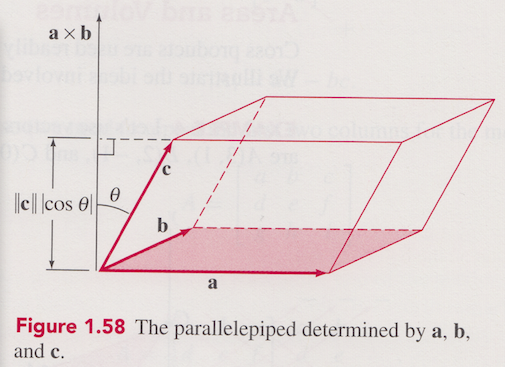
\includegraphics [scale=0.5] {ppd_volume.png} \end{center}
\begin{flushright}Colley \emph{Vector Calculus}\end{flushright}

Recall that the direction of $\mathbf{a} \times \mathbf{b}$ is perpendicular to both vectors.   If we are careful to write the cross-product in the correct order using the right-hand rule, the result of the dot product will always be positive, with the projection of $\mathbf{c}$ onto the cross-product equal to the height of the solid.  In particular, for this arrangement, we must write $\mathbf{a} \times \mathbf{b}$, $\mathbf{b} \times \mathbf{c}$, or $\mathbf{c} \times \mathbf{a}$.

It doesn't matter which two vectors we choose as the base of our solid, the volume must come out the same.
\[ \mathbf{a} \cdot (\mathbf{b} \times \mathbf{c}) = \mathbf{b} \cdot (\mathbf{c} \times \mathbf{a}) = \mathbf{c} \cdot (\mathbf{a} \times \mathbf{b}) \]

The other triple product is
\[ \mathbf{a} \times (\mathbf{b} \times \mathbf{c}) = \]
The components are, in order,
\[ q(sy-tx) - r(ux-sz) \]
\[ r(tz-uy) - p(sy-tx) \]
\[ p(ux-sz) - q(tz-uy) \]
"BACK CAB"
\[ = \mathbf{b} (\mathbf{a} \times \mathbf{c}) - \mathbf{c} (\mathbf{a} \times \mathbf{b}) \]

NEEDS WORK

\chapter{Change of variables}
We usually pick a coordinate system with axes perpendicular, scaled in the same units, with the label $x$ for horizontal and $y$ for vertical.  But for some problems, it can be useful to change the coordinate system.  There are a number of different possible ways to do this, as we'll see.  Importantly, there are some basic rules to follow to insure that the areas determined in the new coordinate system match up with those in the standard one.

Probably the simplest example of this is a linear stretching of one dimension, say, the $x$-axis.  Let's think about the problem of determining the area of the rectangle with one corner at $(0,0)$ and the other corner at $(2,1)$.  Although it seems like overkill, we're going to use (single variable) calculus to do it.  The upper edge is $y = f(x) = 1$.

\[ A = \int_{x=0}^{x=2} f(x)\ dx = \int_0^2 1\ dx = x  \ \bigg |_{0}^{2} = 2 \]

Seems to be correct.  :)

Now, let us define a new variable $u$ which is exchanged at a rate of 2 $u$'s for every $x$.  (If $x=1$ then $u=2$, while if $x=2$ then $u=4$, and so on).
\[ u = 2x \]
We take the exact same shape, (with no change in the area), but change the horizontal coordinate system to be defined in terms of $u$.  The point $(2,1)$ becomes the point $(4,1)$ in the new coordinate system.  So we write
\[ A = \int_{u=0}^{u=4} f(u)\ du  \]
(This is wrong, but bear with me).  You see we have adjusted the limits of integration, since before we had the upper limit of $x=2$, now we have the upper limit of $u=4$.  That part is correct.  $f(x)$ is a constant, so everywhere $f(x) = f(u) = 1$ no matter the value of $x$ (or $u$).  Our mistake is that $du \neq dx$.
\[ du = 2\ dx \]
\[ \frac{1}{2} du = dx \]
so we substitute
\[ A = \int_{x=0}^{x=2} f(x)\ dx =  \int_{u=0}^{u=4} f(u)\ \frac{1}{2}du =  \frac{1}{2} \int_0^4 f(u)\ du = \frac{1}{2} \int_0^4 1\ du =  \frac{1}{2} \times 4 = 2 \]
which is correct.
We can do the very same problem in an even more complicated way, using multi-variable calculus.  Above, we imagine that what we are doing is slicing the area vertically into many slices with tiny width $dx$ and height $f(x)$ and adding all these together.  We can also imagine that we divide the area up into many little boxes of $dA$ and do the summation this way:
\[ A = \iint\limits_{R} 1 \ dA \]
The little boxes of area $dA$ have width $dx$ and height $dy$.
\[ A = \iint\limits_{R} 1 \ dA =   \int_{y=0}^{y=1} \int_{x=0}^{x=2} 1 \ dx \ dy  \]
We evaluate the \emph{inner} integral first, \emph{keeping $y$ constant}.
\[ = \int_{y=0}^{y=1}  x  \ \bigg |_{0}^{2} \ \ \ dy  \]
\[ = \int_{y=0}^{y=1}  2 \ dy  = 2y   \ \bigg |_{0}^{1} = 2  \]
(The real advantage of this is that we can substitute another function for $f(x,y) = 1$---see the Center of Mass write-up).  I introduce the two variable method as a way of approaching the next two problems.

\subsection*{sphere volume by multi-variable calculus}
Before we set up this problem in 3D space, it might help to take a look at the area element in 2D for polar coordinates.

\begin{center} 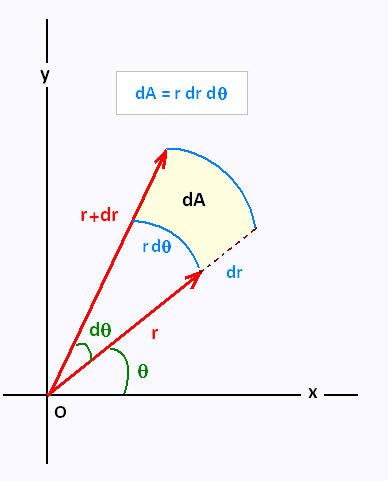
\includegraphics [scale=0.6] {polar_area_element.png} \end{center}
This is the area element dA in the $xy$-plane.  Notice that the little piece of the radius $dr$ is a length, but the little piece of angle $d \theta$ is \emph{not a length}.  To get the length of the curvy part of the area element $dA$, we need to multiply the change in angle by the radius.  So
\[ dA = r d \theta \cdot \ dr \]
(usually written $r \ dr \ d \theta$).  To get an area, you must multiply two lengths.

\url{http://www.scientificsentence.net/Equations/CalculusIII/}

Now, let's try to figure out what the volume elements are for a sphere.
\begin{center} 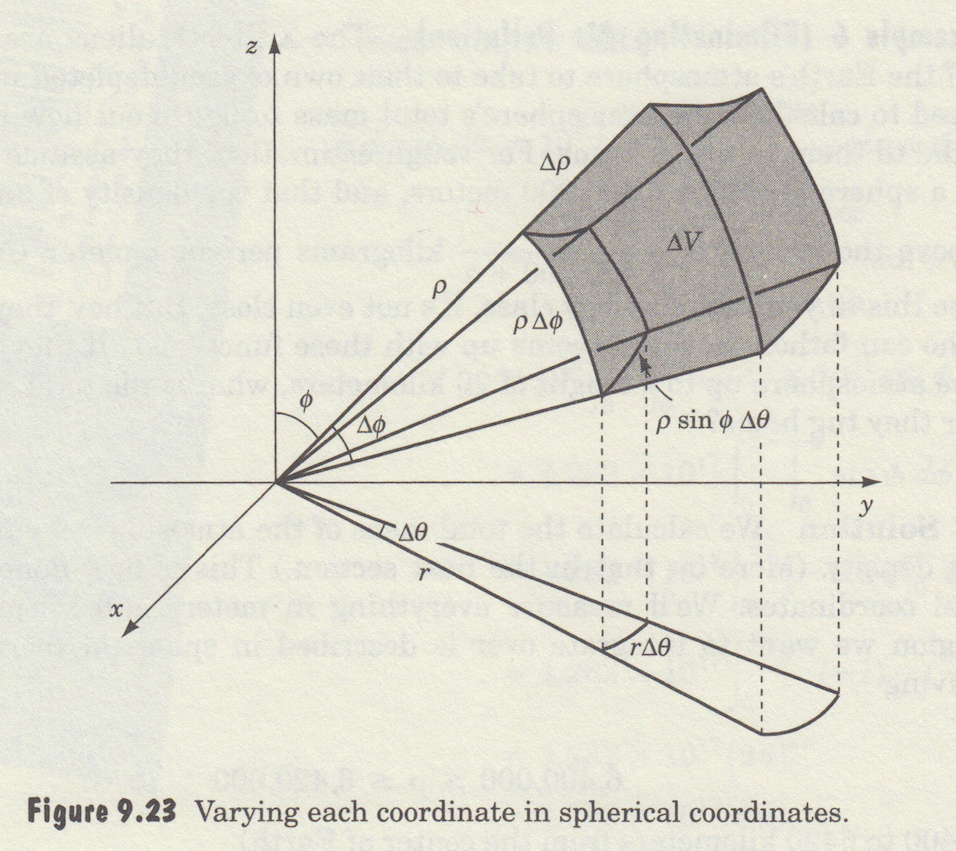
\includegraphics [scale=0.4] {sphcoord.png} \end{center}
The standard way of labeling everything (the parametrization) begins with the polar angle.  This is the angle made by the volume element with the positive $z$-axis.  The mathematicians call this angle $\phi$.  (But the physicists call it $\theta$.  Don't get me started).

The other angle is the standard one from polar coordinates, which is the angle with the positive $x$-axis, or $\theta$.  And for the sphere, usually the radius is denoted by $\rho$ rather than $r$, just to remind us that we are dealing with a sphere.

The two straight sides of the otherwise curvy little box $dV$ lie on the radius, and their length is just $d \rho$.  The two sides which are somewhat vertical here lie on two different great circles, centered on the origin.  We multiply $d \phi$ by the radius $\rho$ to obtain $\rho \ d \phi$.

The tricky ones are those involving $d \theta$.  These also lie on a circle, but not a great circle.  Instead they are horizontal slices through the $z$-axis.  Looking at the projection in the $xy$-plane, you should see that the circle has radius $r$ where $r = \rho \sin \phi$ and therefore the length of these guys is
\[ r \ d \theta = \rho \sin \phi \ d \theta \]

Putting it all together we get two factors of $\rho$ and one of $\sin \phi$ so:
\[ dV = \rho^2 \sin \phi  \ d \rho \ d \phi \ d \theta \]
Getting this is the hard part.

We set up a triple integral
\[ V = \iiint dV \]
\[ = \int_{\theta = 0}^{2 \pi} \int_{\phi = 0}^{\pi}  \int_0^{R} \rho^2 \sin \phi  \ d \rho \ d \phi \ d \theta \]
The integral is easy because the different parts are independent.  The only tricky part is the upper bound on $\phi$, which is equal to $\pi$.  Using independence, we can even rewrite this as
\[ = \int_{\theta = 0}^{2 \pi} d \theta \int_{\phi = 0}^{\pi}  \sin \phi \ d \phi \int_0^{R} \rho^2  \ d \rho \]
We get a factor of $2 \pi$ from the first part and $R^3/3$ from the last, and the middle is
\[ \int_{0}^{\pi}  \sin \phi \ d \phi = - \cos \phi \ \bigg |_{0}^{\pi} = 2\]
Altogether, that is
\[ 2 \pi \cdot \frac{\rho^3}{3} \cdot 2 = \frac{4}{3} \pi R^3 \]

\subsection*{Ellipse}

Let's think about a standard ellipse
\[ \frac{x^2}{a^2} + \frac{y^2}{b^2} = 1 \]
Following the example above, we could think about trying to compute the area of this ellipse as follows
\[ A = \iint\limits_{R} 1 \ dA = \iint\limits_{R} 1 \ dx \ dy \]
The problem is that we do not know how to specify the region, at least, not simply.  However, a little trick can make that problem go away!
\vspace{5 mm}

\noindent
We will change both the horizontal and vertical dimensions by a constant factor.  We compress (well, the opposite of stretching) $x$ by the factor $1/a$ and similarly compress $y$ by the factor $1/b$.  We make a change of variables
\[ x = au\] 
\[ y = bv \]
\[ dx = a\ du \]
\[ dy = b\ dv \]
So 
\[ dx \ dy = ab \ du \ dv \]
Substituting
\[ \frac{(au)^2}{a^2} + \frac{(bv)^2}{b^2} = u^2 + v^2 = 1\]
The substitution has converted the ellipse into a circle of radius $1$ and area $A = \pi$.
and
\[ A = \iint\limits_{R} 1 \ dx \ dy =  \iint\limits_{R} ab \ du \ dv = ab \iint\limits_{R} 1 \ du \ dv \]
Now, we know the area of the region in $u,v$ coordinates, it is a circle of radius $1$ and its area is just equal to $\pi$.  So finally
\[ A = ab \iint\limits_{R} 1 \ du \ dv = \pi a b \]
This is a really simple, beautiful result.  The two $r$'s in the formula $A= \pi r^2$ become $a \times b$.  Both dimensions make equivalent contributions to the area, as we'd expect.
\vspace{5 mm}

\noindent
The more formal way to do this is to compute what's called the Jacobian.  It gives the ratio between areas determined in two different coordinate systems.  We take the partial derivative of $x$ with respect to $u$ and $v$, and similarly for $y$.
\[ x_u = a \]
\[ x_v = 0 \]
\[ y_u = 0 \]
\[ y_v = b \]
The two partials ($x_v$ and $y_u$) are zero because $x$ does not depend on $v$ and  $y$ does not depend on $u$.

We evaluate the determinant of this matrix:
\[ J = 
\begin{vmatrix}
x_u & x_v \\
y_u & y_v 
\end{vmatrix} =
\begin{vmatrix}
a & 0 \\
0 & b
\end{vmatrix} =ab
\]
And that's the factor for converting between the two coordinate systems.
Sometimes the Jacobian is written as
\[ J = 
\begin{vmatrix}
x_u & y_u \\
x_v & y_v 
\end{vmatrix}
\]
but this doesn't change anything, because $det(A) = det(A^T)$.

To summarize:
\[ dx \ dy = J \ du \ dv \]
where
$J$ is computed as described.

\subsection*{Circle}

Another simple example is to find the area of a circle of radius $a$.  In terms of $x$ and $y$ we had previously
\[  \iint\limits_{R}  \ dA = \int_{x=0}^{x=a} \int_{y=0}^{y=\sqrt{a^2-x^2}} \ dy \ dx = \int_{x=0}^{x=a} \sqrt{a^2-x^2}  \ dx \]
This integral can be computed by doing a trig substitution, but there is an easier way, and that is to change to polar coordinates.  A naive attempt is
\[  \iint\limits_{R}  \ dA = \int_{\theta=0}^{\theta=2 \pi} \int_{r=0}^{r=a} \ dr \ d \theta = \int_{\theta=0}^{\theta=2 \pi} a \ d \theta = 2 \pi a \]
Obviously, this is wrong.
What happened is that the area element for a little bit of area $dA$ has an extra factor of $r$:

\[ dA = dx \ dy = r \ dr \ d \theta \]

\begin{center} 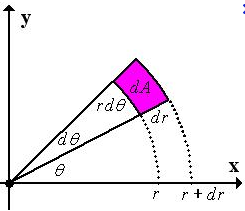
\includegraphics [scale=0.6] {polararea.png} \end{center}
As Strang says "areas always come from multiplying two lengths, and $d\theta$ is not a length."  He goes on to say that a wedge has area
\[ A = \frac{1}{2} r^2 \Delta \theta \]
The difference between wedges is $\Delta A$, and centering the change $\Delta r$ at $r$ we have:
\[ \Delta A = \frac{1}{2}(r + \frac{\Delta r}{2})^2 \Delta \theta - \frac{1}{2}(r - \frac{\Delta r}{2})^2 \Delta \theta \]
\[ = \frac{1}{2}(r^2 + r \Delta r + \frac{\Delta r^2}{4}) \Delta \theta - \frac{1}{2}(r^2 - r \Delta r + \frac{\Delta r^2}{4}) \Delta \theta \]
Neglecting the small term $\Delta r^2$:

\[ \Delta A =  r \Delta r \Delta \theta \]
The length of the curvy segment of arc depends on how far out we are on the radius.
\[ \iint\limits_{R}  \ dA = \int_{\theta=0}^{\theta=2 \pi} \int_{r=0}^{r=a} \ r \ dr \ d \theta = \int_{\theta=0}^{\theta=2 \pi} \frac{1}{2}a^2 \ d \theta = \pi a^2 \]
The Jacobian is done like this: 
\[ x = r\ cos\ \theta, \ \ y = r\ sin\ \theta \]
For convenience I'll define
\[ x_r = \frac{\partial x}{\partial r} = cos \ \theta, \ \ x_{\theta} = \frac{\partial x}{\partial \theta} = -r \ sin \ \theta \]
and similarly for $y$.  Then
\[ J = 
\begin{vmatrix}
x_r & x_{\theta} \\
y_r & y_{\theta} 
\end{vmatrix} =
\begin{vmatrix}
\cos\ \theta & -r \ sin\ \theta \\
\sin\ \theta & r \ cos\ \theta 
\end{vmatrix} = r (cos^2\ \theta + sin^2\ \theta) = r
\]
This is the factor for the ratio of areas under the two systems, and that's why we have $r\ dr \ d\theta$ in the integral.  Notice that when we took the partial derivatives, they were partials of $x,y$ with respect to $r,\theta$, and we end up multiplying $dr \ d\theta$ by J.

\subsection*{General method}

Suppose we wish to determine an area by integration and we're working with the unit square $x=0 \to x=1$ and $y=0 \to y=1$, sometimes written as $[\ 0,1\ ] \times [\ 0,1\ ]$.  The area is clearly just $1$.  Now we want to make a change of variables for some reason (to work on a function that's easier to deal with, or because we have some weird bounds in our problem).
\[ u = 3x-2y , \ \ v = x + y \]
We can figure out the "exchange rate" by tracing out the parallelogram formed by this linear transformation

\begin{align*}
& (0,0) \to (0,0) \\
& (0,1) \to (3,1) \\
& (1,1) \to (1,2) \\
& (0,1) \to (-2,1)
\end{align*}

If we think of the vectors $<3,1>$ and $<-2,1>$, the area of the parallelogram formed by these vectors is given by the determinant
\[
\begin{vmatrix}
3 & -2 \\
1 & \ \ 1 
\end{vmatrix} = 5
\]
The other way to do this calculation is (as we've been doing)
\[ u_x = 3 \]
\[ u_y = -2 \]
\[ v_x = 1 \]
\[ v_y = 1 \]
The Jacobian
\[ J = 
\begin{vmatrix}
u_x & u_y \\
v_x & v_y 
\end{vmatrix} = 
\begin{vmatrix}
3 & -2 \\
1 & \ \ 1 
\end{vmatrix}
= 3 - (-2) = 5 \]
Or more simply
\[ J = u_x v_y - u_y v_x = 3  - (-2) = 5 \]
And again, since we took the derivatives with respect to $x$ and $y$, we multiply $dx \ dy$ by $J$.

Each element of the area determined in $uv$ units is worth $5$ of an element in $xy$ units.
\[ 5 \iint\limits_{R}  f(x,y) \ dx \ dy = \iint\limits_{R}  f(u,v) \ du \ dv \]
\begin{equation}
\boxed{du \ dv = J \ dx \ dy }
\end{equation}
\vspace{5 mm}

\noindent
To say the above one more time in slightly different language, we have
\[ u = u(x,y) \]
\[ v = v(x,y) \]
If we change $x$ by a little bit $\Delta x$ and $y$ by a little bit $\Delta y$, by how much do $u$ and $v$ change? 
The linear approximation is
\[ \Delta u = u_x \Delta x + u_y \Delta y \]
\[ \Delta v = v_x \Delta x + v_y \Delta y \]
So for $\Delta x = 1$, the vector $<1,0>$ becomes
\[ \ <u_x ,v_x> \]
and $<0,1>$ becomes
\[ \ <u_y ,v_y> \]
and the area of the parallelogram formed by these two vectors (the area in $uv$-coordinates) is the absolute value of the cross product (think of them as lying in the plane, so there is only one term)
\[ <u_x ,v_x> \ \times  <u_y ,v_y > \]
\[ J = u_x v_y - u_y v_x \]
So for each unit $dx \ dy$ we get $du \ dv = J \ dx \ dy $ in the $uv$-coordinate system.

\subsection*{Tilted ellipse}
Here is the equation of an ellipse, although that may be hard to recognize at first.
\[ x^2 + 4xy + 13y^2 = 16 \]
If you remember (or look up) the formula
\[ Ax^2 + Bxy + Cy^2 + Dx + Ey + F = 0 \]
\[ A,B,C = 1,4,13 \]
The discriminant is
\[ B^2 - 4AC = 16 - 52 = -36 < 0 \]
Since it's $ < 0 $, this is an ellipse.  Or we could just get Grapher to plot it
\begin{center} 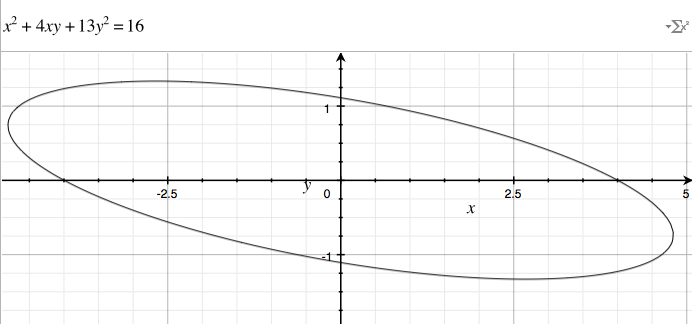
\includegraphics [scale=0.4] {tilted_ellipse.png} \end{center}
If we knew the angle, and there is a method for that, we could rotate to a new coordinate system and just compute the area as $\pi ab$.  However, there is another way which I think is easier.  We "complete the square" to remove the term which "mixes" $x$ and $y$.  Since
\[ (x + 2y)^2 = x^2 + 4xy + 4y^2 \]
Our equation is transformed as follows
\[ x^2 + 4xy + 13y^2 = 16 \]
\[ (x + 2y)^2 + 9y^2 = 16 \]
We do a substitution almost like before, but modified:
\[ u = x + 2y \]
\[ v = 3y \]
so now we have
\[ u^2 + v^2 = 16 \]
This is a circle of radius $4$ and area $16\pi$.
Now we just need the Jacobian:
\[ u_x = 1 \]
\[ u_y = 2 \]
\[ v_x = 0 \]
\[ v_y = 3 \]
\[ J = 
\begin{vmatrix}
u_x & u_y \\
v_x & v_y 
\end{vmatrix} = 
\begin{vmatrix}
1 & 2 \\
0 & 3 
\end{vmatrix}
= 3 \]
\[ du \ dv = 3 \ dx \ dy \]
When we took the partial derivatives, they were partials of $u,v$ with respect to $x,y$, so we end up multiplying $dx \ dy$ by J.
\[ \frac{1}{3} du \ dv = dx \ dy \]
We need to multiply the area by this factor to give a final answer of $16\pi/3$.

\subsection*{Varberg's example}
The next example is from Varberg, 17.16.
\begin{center} 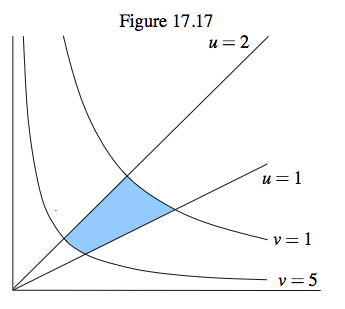
\includegraphics [scale=0.6] {Varberg-17-16.png} \end{center}
We have the lines $x=y$ and $x=2y$ and the curves $xy=1$ and $xy=5$.  Looks like $xy$ would be a good variable to have so
\[ u = \frac{x}{y} \]
\[ v = xy \]
These suggestions come from Varberg, not me.  :)  The boundaries of the region are just $u = 1 \rightarrow u = 2$ and $v = 1 \rightarrow v = 5 $.
Rearranging:
\[ x = uy \]
\[ x = \frac{v}{y} \]
\[ x^2 = xx = uy \ \frac{v}{y} =  uv \]

For the Jacobian, it is important to solve for $x,y$ in terms of $u,v$, and not the other way around, so that we'll have terms containing $u$ and $v$ in the final integral.
\[ x = \sqrt{uv} \]
\[ y^2 = \frac{x}{u} \frac{v}{x} = \frac{v}{u} \]
\[ y = \sqrt{\frac{v}{u}} \]
So 
\[ x_u = \frac{1}{2} \sqrt{\frac{v}{u}} \]
\[ x_v =  \frac{1}{2} \sqrt{\frac{u}{v}} \]
\[ y_u =  -\frac{1}{2u} \sqrt{\frac{v}{u}}\]
\[ y_v = \frac{1}{2} \sqrt{\frac{1}{uv}} \]
The Jacobian is then
\[ x_u y_v - x_v y_u \]
\[ \frac{1}{2} \sqrt{\frac{v}{u}} \ \frac{1}{2} \sqrt{\frac{1}{uv}} + \frac{1}{2} \sqrt{\frac{u}{v}} \  \frac{1}{2u} \sqrt{\frac{v}{u}} \]
\[ = \frac{1}{4u} + \frac{1}{4u} = \frac{1}{2u} \]
The area is 
\[ A = \iint\limits_{R} 1 \ dx \ dy =  \iint\limits_{R} \frac{1}{2u}  \ du \ dv \]
\[ = \int_{u=1}^{2} \ \int_{v=1}^{5} \frac{1}{2u}  \ dv \ du \]
\[ = 2 \int_{u=1}^{2} \ \frac{1}{u} \ du = 2 \ln 2 \]

\subsection*{Even weirder example from Auroux}

Suppose we have 
\[ \int_{y=0}^1 \int_{x=0}^1 x^2 y \ dx \ dy \]
For some strange reason we've decided that we're going to change to
\[ u = x, \ \ v = xy \]
\[ u_x = 1, \ \ u_y = 0, \ \ v_x = y, \ \ v_y = x \]
\[ J = 
\begin{vmatrix}
1 & 0 \\
y & x 
\end{vmatrix} = x \]

\[ du \ dv = x \ dx \ dy \]
\[ \iint\ xy \ x \ dx \ dy =  \iint\ v \ du \ dv  \]
That looks OK, but what are the limits?
\begin{center} 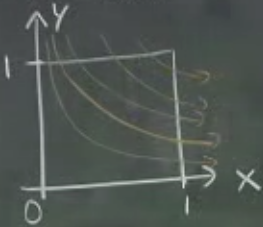
\includegraphics [scale=0.4] {changevar1.png} \end{center}
The first integral is with $v$ constant.  That means $xy=v$ is a constant, so we have different curves $xy = const$ (i.e. hyperobolas) between some limits.  The slices look like those in the figure above.

We enter our region from the top

\[ y= 1 \Longrightarrow u = x, v = xy = x = u \]
We leave the region on the side
\[ x= 1 \Longrightarrow u = 1 \]
\[ \int \int_{u=v}^{u=1} v \ du \ dv \]
The smallest value of $v$ is 
\[ x = 0 \Longrightarrow v = 0 \]
The largest value of $v$ is 
\[ x = 1, y = 1 \Longrightarrow v = 1 \]
\[ \int_{v=0}^{v=1} \int_{u=v}^{u=1} v \ du \ dv \]
The inner integral is 
\[ \int_{u=v}^{u=1} v \ du = uv \ \bigg |_{u=v}^{u=1} = v - v^2 \]
and the outer integral is
\[ \int_{v=0}^{v=1} v - v^2 \ dv = \frac{1}{2}v^2 - \frac{1}{3}v^3 \ \bigg |_{0}^{1} = \frac{1}{2} - \frac{1}{3} = \frac{1}{6} \]
We may have some doubt about the answer, so going back to what we started with and doing the integral we have
\[ \int_{y=0}^1 \int_{x=0}^1 x^2 y \ dx \ dy \]
The inner integral is 
\[ \int_{x=0}^1 x^2 y \ dx = \frac{1}{3}x^3y \ \bigg |_{0}^{1} = \frac{1}{3}y  \]
and the outer integral is
\[ \int_{y=0}^1  \frac{1}{3}y \ dy = \frac{1}{6}y^2 \ \bigg |_{0}^{1} = \frac{1}{6}  \]
which agrees.

\chapter{Line integrals}

A simple application of a line integral is to find the length of a curve.  A more sophisticated one yields the work done when moving along a curve, and there are certainly others.

The basic formula can be derived by doing algebra with differentials.  Think of a small element of the path of the curve, $ds$, as a right triangle with side lengths $dx$ and $dy$.  Then

\[ ds^2 = dx^2 + dy^2 \]

We "divide and multiply" on the right by $dx^2$ to give

\[ ds^2 = [1 + \frac{dy^2}{dx^2}] \ dx^2 \]

then take the square root

\[ ds = \sqrt{1 + (\frac{dy}{dx})^2} \ dx \]
\[ ds = \sqrt{1 + (y')^2} \ dx \]

In many cases $x$ and $y$ will be parametric equations (functions of a parameter like $t$), or we might just express $y$ in terms of $x$.  In any case, the integral will be of a single variable.
\subsection*{Example 0}
Here is one where we already know the answer:  the arc length along the boundary of the circle of radius $R$ in the first quadrant.  Again, the formula is
\[ ds = \sqrt{1 + (\frac{dy}{dx})^2} \ dx \]
So we want
\[ L = \int ds = \int_0^R  \sqrt{1 + (\frac{dy}{dx})^2} \ dx \]
The circle is
\[ x^2 + y^2 = R^2 \]

By implicit differentiation, we easily obtain
\[ 2x \ dx + 2y \ dy = 0 \]
\[ \frac{dy}{dx} = -\frac{x}{y} \]
\[ (\frac{dy}{dx})^2 = \frac{x^2}{y^2} \]
So the integral is
\[ = \int_0^R  \sqrt{1 + \frac{x^2}{y^2}} \ dx \]
\[ = \int_0^R \frac{1}{y}  \sqrt{y^2 + x^2} \ dx \]
\[ = R \int_0^R \frac{1}{y}  \ dx \]
\[ = R \int_0^R \frac{1}{\sqrt{R^2-x^2}}  \ dx \]

This can be solved by a trig substitution:
\[ x = R \sin t \]
\[ dx = R \cos t \ dt \]
\[ \sqrt{R^2 - x^2} = R \cos t \]
So we have
\[ = R \int \frac{1}{R \cos t} R \cos t \ dt = R t \]
The slightly tricky part is the limits on $t$.  The lower limit was $x=0$, so now we need $R \sin t = 0$, so $t=0$.  And the upper limit was $x=R$, so now we need $R \sin t = R$ so $t = \pi/2$.  The integral is $\pi R/2$ and the whole circumference is $4$ times that or $C = 2 \pi R$.

Another, simpler way to do this calculation is to use the parametrized circle ($x = \cos \theta, y = \sin \theta$).  Go back to the original definition of the element of arc $ds$:

\[ ds^2 = dx^2 + dy^2 \]
\[ L = \int ds = \int \sqrt{dx^2 + dy^2} \]
\[ = \int \sqrt{\cos^2 \theta + \sin^2 \theta} \ d \theta \]
\[ = \int \ d \theta \]

Here, we can just go all the way around the circle from $\theta = 0 \Rightarrow 2 \pi$.  And for a circle of radius $a$ we have $a \cos \theta$ and $a \sin \theta$ which gives a factor of $a^2$ under the square root, yielding an extra factor of $a$ in the end.

\subsection*{Example 1}
Consider
\[ y = x^2 \]
\[ \frac{dy}{dx} = 2x \]
\[ ds = \sqrt{1 + (\frac{dy}{dx})^2} \ dx \]
\[ ds =  \sqrt{1 + 4x^2} \ dx \]

The arc length is the integral of $ds$

\[ L = \int  \sqrt{1 + 4x^2} \ dx \]
\[ = 2 \int  \sqrt{(\frac{1}{2})^2 + x^2} \ dx \]

This will be a minor challenge (see trig substitutions).  Rather than struggle with it, just set $a = \frac{1}{2}$ and look up the answer in a table of integrals

\[ \int  \sqrt{a^2 + x^2} \ dx  = \frac{x}{2}\sqrt{a^2 + x^2} + \frac{a^2}{2} \ln \ | \ x + \sqrt{a^2 + x^2} \ | \]

substitute back for $a = 1/2$

\[ \frac{x}{2}\sqrt{\frac{1}{4} + x^2} + \frac{1}{8} \ln \ | \ x + \sqrt{\frac{1}{4} + x^2} \ | \]

Suppose the limits are $x=1$ and $x=0$.  At the upper limit, we have

\[ \frac{1}{2}(\sqrt{1.25}) + \frac{1}{8} \ \ln \ (1 + \sqrt{1.25}) \] 
\[ \sqrt{1.25} \approx 1.118  \]
\[ \ln (2.118) \approx 0.7505 \]
\[ (0.5)(1.118) + (0.125)(0.7505) = 0.559 + 0.0938 = 0.6528 \]

while at the lower limit the first term is $0$ and the second is

\[ \frac{1}{8}\  \ln \frac{1}{2} = - (0.125)\  \ln 2 = - (0.125)(0.693) = -0.0866 \] 

Subtracting

\[ 0.6528 + 0.0866 = 0.7394 \]

Remembering the factor of two we get $1.4788$

Not exactly pretty, but it works.  Check by numerical integration

\begin{verbatim}
import scipy
f = lambda x: x**2
scipy.integrate.quad(f,0,1)
\end{verbatim}
This check gives the expected result $ 0.33333..$

\begin{verbatim}
g = lambda x: sqrt(1 + 4*x**2)
scipy.integrate.quad(g,0,1)
\end{verbatim}
results in $1.47894$

\subsection*{Example 2}
Most commonly, however, we have $x$ and $y$ as functions of a parameter $t$.  Also we may have a vector field $\mathbf{F}$ where
\[ \mathbf{F} = \langle \ M,N \ \rangle \]
or
\[ \mathbf{F} = \langle \ M,N,P \ \rangle \]
and we are interested in the integral along the curve (for the work done by $\mathbf{F}$):
\[ \int_C \mathbf{F} \cdot d\mathbf{r} = \int_C F \cdot \hat{\mathbf{T}} ds \]
\[ = \int_C M \ dx + N \ dy + P \ dz \]
This last part seems like a magic trick.  We'll see how it's done in the next section.

Here I would like to show how we evaluate it.  The crucial insight is parametrization of the curve.  Suppose
\[ \mathbf{F} = \langle \ x,y,z \ \rangle \]
and we have equations for $x(t), y(t), z(t)$
\[ x = t, \ \ \ \ y = t, \ \ \ \ z = 2t^2 \]
\[\frac{d\mathbf{r}}{dt} = \ \langle \ \frac{dx}{dt},\frac{dy}{dt},\frac{dz}{dt} \ \rangle \]
\[ = \ \langle \ 1,1,4t \ \rangle \]\[ \int_C \mathbf{F} \cdot dr \int \mathbf{F} \cdot \frac{d\mathbf{r}}{dt} \ dt = \int_C \ \langle \ t,t,2t^2 \ \rangle \  \cdot \ \langle \ 1,1,4t \ \rangle \ dt \]
\[ = \int_C (2t + 8t^3) dt = t^2 + 2t^4 \]
Evaluate from say, $t=0$ to $t=1$
\[  t^2 + 2t^4 = 3 \]
It doesn't seem complicated at all, once we have the parametric equations.
\vspace{2 mm}

\subsection*{Work}
The basic line integral is something like this one for work
\[ W = \int_C \mathbf{F} \cdot d\mathbf{r} \]
We have a curve $C$ made up of lots of little pieces $d\mathbf{r}$.  For each piece, we compute the dot product with the force $\mathbf{F}$, multiplying by the component of the force that is in the same direction as we're headed.  

As before, it makes great sense symbolically, but how to compute it?  To start with do
\[ d\mathbf{r} = \hat{\mathbf{T}} \ ds \]
where $\hat{\mathbf{T}}$ is the unit vector in the direction of $d\mathbf{r}$ and $ds$ is the magnitude of $d\mathbf{r}$.  Moreover, notice that
\[ \frac{d\mathbf{r}}{dt} = \mathbf{v} = \hat{\mathbf{T}} \ \frac{ds}{dt} \]
so
\[  \int_C \mathbf{F} \cdot d\mathbf{r} =  \int_C \mathbf{F} \cdot \mathbf{v} \ dt =  \int_C \mathbf{F} \cdot \mathbf{T}\ \frac{ds}{dt} \ dt  \]
If $\mathbf{F}$ has components
\[ \mathbf{F} = \ \langle \ M,N \ \rangle \]
then this becomes
\[  \int_C  \ \langle \ M,N \ \rangle \ \cdot \ \langle \ \frac{dx}{dt},\frac{dy}{dt} \ \rangle \ dt \]
We could even write this
\[  \int_C  M \ dx + N \ dy \]

This is a useful mnemonic, but remember that this is a single integral, and we can't just do $dx$ and $dy$ separately.  We need a single variable and $t$, the parameter for the curve $C$, comes to the rescue.  (Either that or $y=f(x)$).  We must get all these in terms of $t$.  Then it's OK.  Also, it may be necessary to break the curve up into pieces.
Suppose $C$ is the unit square and 
\[ \mathbf{F} = \ <x,y> \ \]

For the first leg we have $y=0$ and $x=0 \rightarrow 1$.  So parametrize $x$ using $t$ by setting $x=t$ and let $t=0 \rightarrow 1$.  Now
\[ dx/dt = 1 \] 
and 
\[ dy/dt=0 \]
 and since $\mathbf{F} = \ <x,y>$;  $M = x = t$)
 \[   \int_C  \ <M,N> \ \cdot \ <\frac{dx}{dt},\frac{dy}{dt}> \ dt = \int M dt \]
\[ = \int t \ dt \ \bigg|_0^1 \]
\[ = \frac{1}{2} \]
In a similar way, on the second leg (up to $(1,1)$)
\[ dx/dt=0 \]
 and 
 \[ dy/dt=1 \]
 and we have exactly the same integral.

For the third and fourth legs, we get a minus sign (because $x$ and $y$ are equal to minus $t$), but again the absolute value of the integral is $\frac{1}{2}$, and in the end the total work is 0.

That's interesting, why is the total work zero?  It turns out to be because our force $\mathbf{F} = \ <x,y>$ is the gradient of a potential function.  
\[ \mathbf{F} = \nabla \mathbf{f} \]
where
\[ \nabla = \ < \ \frac{\partial }{\partial  x},\frac{\partial }{\partial  y},\frac{\partial }{\partial  z} > \]
Can we guess what function? Sure!
\[ f(x,y) = \frac{1}{2}x^2 + \frac{1}{2}y^2 \]
That gives the correct values for the components of $\mathbf{F}$
\[ \mathbf{F} = \nabla \mathbf{f} = \nabla ( \frac{1}{2}x^2 + \frac{1}{2}y^2) = \ <f_x,f_y> \ = \ <x,y> \]
and since 
\[  \hat{\mathbf{T}} \ ds = (dx\ \hat{\mathbf{i}} + dy\ \hat{\mathbf{j}}) \]
Then, at least in the case where this gradient condition holds, we have

\[ \int_C \mathbf{F} \cdot  \hat{\mathbf{T}} \ ds  = \ <f_x,f_y> \  \cdot  (dx\ \hat{\mathbf{i}} + dy\ \hat{\mathbf{j}})  \] 
written with the "del" notation
\[= (\frac{\partial f}{\partial  x} \hat{\mathbf{i}} + \frac{\partial f}{\partial  y} \hat{\mathbf{j}}) \cdot (dx\ \hat{\mathbf{i}} + dy\ \hat{\mathbf{j}}) \]
\[ = \frac{\partial f}{\partial  x} \ dx + \frac{\partial f}{\partial  y} \ dy \]
\[ = df \]
\subsection*{another example}
Suppose $\mathbf{F}$ is $<y,x> $ and we want
\[ \int_C \mathbf{F} \cdot  \hat{\mathbf{T}} \ ds \]
\[ = \int_C y \ dx + x \ dy \]

$C$ is a sector of the unit circle between $0 <= \theta <= \pi/4$.  We break the curve up into 3 parts.
$C_1$, from $(0,0)$ to $(0,1)$.  As before, notice that $y=0$, so $dy=0$ and 
\[ \int_C y \ dx + x \ dy = 0 \]
Also, notice that $\mathbf{F}$ is $<0,x>$, so $\mathbf{F} \perp d\mathbf{r}$ and then  $\mathbf{F} \cdot d\mathbf{r} = 0$.

For $C_2$ from $(0,1)$ to $(1,0)$  Here, we're on the unit circle.  It's natural to change variables:

\[ x = \cos \ \theta \]
\[ dx = -sin \ \theta \ d \theta \]
\[ y = \sin \ \theta \]
\[ dy = \cos \ \theta \ d \theta \]

\[ \int_C y \ dx + x \ dy  \]
\[ = \int_C -\sin^2 \theta \ d \theta + \cos^2 \theta \ d \theta \]
\[ = \int_C \cos \ 2 \theta \ d \theta \]
\[ = \frac{1}{2} \sin \ 2 \theta \ \bigg|_0^{\pi/4} \]
\[ = \frac{1}{2} \]

For $C_2$ from $(1,0)$ back to $(0,0$, we could do $x=y=t$, but we don't need $t$, instead just use $x=y$ and $dx=dy$ then
\[ \int_C y \ dx + x \ dy  \]
\[ 2 \int_C x \ dx \]
\[ = x^2  \ \bigg|_{1/\sqrt{2}}^0 \]
\[ = \frac{1}{2} \]

So, once again, the total integral is $0$.

And the reason is that $\mathbf{F}$ is (again) the gradient ($\nabla$) of a potential function.  By guessing, we obtain this formula for the potential:

\[ f(x,y) = xy \]
\[ F = \nabla f = \ < \ f_x,f_y \ > \ = \ < \ y,x \ > \]

The fundamental theorem of calculus for line integrals:

 \[ \int_C \nabla f \cdot d \mathbf{r} =   f(P1) - f(P2) \]
  
The example is a closed curve (P1 = P2), so of course it's just 0.  But we can also do each part separately using the method.  We get $f(x,y) = (1/\sqrt{2} \times 1/\sqrt{2}) = 1/2$ along $C_2$ (starting from $0$ at $C_1$), and of course, minus that along $C_3$, back to $(0,0)$.

In the case where $\mathbf{F}$ is the gradient ($\nabla$) of a potential function
\[ \mathbf{F} \cdot \hat{\mathbf{T}} ds = (f_x \ \hat{\mathbf{i}} + f_y \ \hat{\mathbf{j}}) \cdot (dx \ \hat{\mathbf{i}} + dy \ \hat{\mathbf{j}} ) \]

\chapter{Cycloid}

We imagine a bicycle with one tire marked at a particular point on the rim, say with fluorescent paint or a small light.  We start at time $t = 0$ with that point $P$ in contact with the $x$ axis at $(0,0)$.  Then we start rolling the bike.  As the tire rotates our fixed point $P$ on the rim traces a curve
\begin{center} 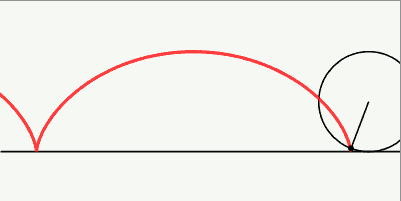
\includegraphics [scale=0.6] {cycloid.png} \end{center}

\begin{center} 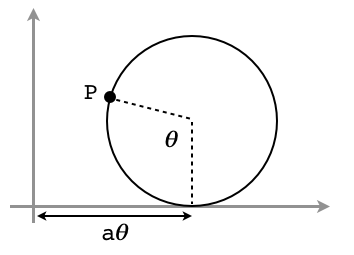
\includegraphics [scale=0.5] {cycloid2.png} \end{center}
We want to find parametric equations $x(t)$, $y(t)$ that give the position of the point $P$ as a function of time.  The second diagram above shows the angle through which the wheel has turned as $\theta$, but we will use $t$ for $\theta$ here.  The $x$ displacement of the vertical straight down from the center of the tire is just $at$, where $a$ is the radius of the wheel, it is equal to the arc on the circumference of the wheel from the point which is currently in contact with the ground, up to $P$.

It is fairly easy to derive the desired parametric equations, using vectors.  For $x$, we have the vector that goes from $(0,0)$ to the contact point with the ground.  As indicated in the figure, that is $at$.  We need to subtract the distance $a \ sin\ t$ from that.  It's easier to see for $t < \pi/2$, but it is true always.  This is the usual circular motion, just with the circle flipped so the motion is clockwise, and we started at the bottom.

For $y$, we have a constant factor of $a$ above the $x$ axis, then the additional displacement is $-a \ cos \ t$.  So for $t=0$ we have the additional displacement is -a (we were on the ground), for $t=\pi/2$ it is zero, and for $t=\pi$ it is plus $a$ for a total of $2a$.

The parametric equations are then
\begin{align*} 
x(t) = at - a \ sin\ t \\
y(t) = a - a \ cos\ t \\
x'(t) = a - a \ cos\ t \\
y'(t) = a \ sin\ t  \\
\end{align*} 

The derivation above did a little mental gymnastics with the circle, flipping it and setting $t=0$ when the point is at the bottom.  As an alternative, leave the circle in its usual orientation, with an angle $s$ to the positive $x$ axis.

It can be seen easily that $s$ and $t$ are related by the equation 
\[ s = 3\pi/2 - t \]

The vector from the center of the circle to the point on the edge is just the standard one for a point on a circle of radius $a$:
\[ a \ \langle \cos s, \sin s  \rangle \]
For the $x$ component:
\[ \cos s = \cos 3 \pi / 2 - t \]
\[ = \cos 3 \pi / 2  \cos t + \sin 3 \pi / 2 \sin t \]
Recall that $\cos 3 \pi / 2 = 0$ and $\sin 3 \pi / 2 = -1$ so
\[ \cos s = - \sin t \]
And for the $y$ component
\[ \sin s = \sin 3 \pi / 2 - t \]
\[ = \sin 3 \pi / 2 \cos t - \sin t \cos  3 \pi / 2 \]
\[ = - \cos t \]
The vector is then
\[ a \ \langle \cos s, \sin s  \rangle = a \ \langle -\sin t, -\cos t  \rangle \]

In addition, we have to add another vector, one extending from the origin to the center of the wheel.  The $y$ component is constant, it is just $a$.  The $x$-component is the distance the wheel has traveled from its initial position (the distance between the origin and the point of contact with the $x$-axis, which is $at$, shown as $a \theta$ in the figure).

Hence the vector to the point is:
\[ a \ \langle -\sin t, -\cos t  \rangle + \langle at, a \rangle \]
\[ a \ \langle t - \sin t, 1 - \cos t \rangle \]

which matches what we had before.

\subsection*{Arc length}

We wish to determine the arc length and area under the curve for a complete revolution of the wheel.

We want to use a slightly different version of the usual formula for arc length

\[ ds^2 = dx^2 + dy^2 \]
\[ (\frac{ds}{dt})^2 = (\frac{dx}{dt})^2 + (\frac{dy}{dt})^2 \]
\[ ds = \sqrt{(\frac{dx}{dt})^2 + (\frac{dy}{dt})^2} \ dt = \sqrt{(a - a \cos\ t)^2 + (a \sin\ t)^2} \ dt  \]
This expands to
\[ a \sqrt{1 - 2 \cos\ t + \cos^2t + \sin^2t } \ dt =  a \sqrt{2 - 2 \cos \ t} \ dt\] 
The length is
\[ L = \int_0^{2\pi} a \sqrt{2 - 2 \cos \ t} \ dt\]
\[ = a \sqrt{2} \ \int_0^{2\pi} \sqrt{1 - \cos \ t} \ dt\]

\subsection*{double angle}

\[ \cos (s-t) = \cos s \cos t + \sin s \sin \ t \]
(check:  if $s=t$ then $\cos 0 = 1$, which is correct).

So
\[ \cos (s+t) = \cos s \cos t - \sin s \sin \ t \]
Let $s = t$ and $u = 2s$, then
\[ \cos 2s = \cos u = \cos^2 \ (\frac{u}{2}) - \sin^2 \ (\frac{u}{2}) \]
\[ \cos u = 1 - \sin^2 \ (\frac{u}{2}) - \sin^2 \ (\frac{u}{2}) \]
\[ 2 \sin^2 \ (\frac{u}{2}) = 1 - \cos u \]
$u$ is just a dummy variable, so we can switch back to $t$
\[ 2 \sin^2 \ (\frac{t}{2}) = 1 - \cos t \]

\subsection*{finishing up}
We have that 
\[ L = a \sqrt{2} \ \int_0^{2\pi} \sqrt{1 - \cos \ t} \ dt\]

\[ 1 - \cos t = 2 \sin^2(\frac{t}{2}) \]
\[ \sqrt{1 - \cos t} = \sqrt{2} \sin(\frac{t}{2}) \]
So
\[ L = a \sqrt{2} \ \int_0^{2\pi} \sqrt{2} \sin \ (\frac{t}{2}) \ dt\]
\[  2a  \ \int_0^{2\pi} \sin \ (\frac{t}{2}) \ dt\]
\[ = 2a \ (-2) \cos \ (\frac{t}{2})\ \bigg |_0^{2\pi} \]
\[ = -4a \ (\cos \ \pi - \cos \ 0) \]
\[ = -4a \ (-1 - 1) = 8a\]
A simple answer to the problem.

\subsection*{Area under the arc}
We want
\[ A = \int_{t=0}^{t=2\pi} y \ dx \]
\[ = \int_{t=0}^{t=2\pi} (a - a \cos\ t) (a - a \cos\ t) \ dt \]
\[ a^2\int_{t=0}^{t=2\pi} (1 - \cos\ t) (1 - \cos\ t) \ dt \]
\[ a^2\int_{t=0}^{t=2\pi} (1 - 2 \cos\ t + \cos^2\ t) \ dt \]
If you don't remember the result for $\int \cos^2 t \ dt$, you can go back to the double angle formula above and convert from $\sin^2$ to $\cos^2$.  Otherwise recall it and write:
\[ A = a^2 ( t - 2 \sin \ t + \frac{1}{2}t + \frac{1}{4} \sin 2t ) \ \bigg|_0^{2\pi} \]
\[ a^2 ( 2\pi - 0 + \pi + 0 - 0 + 0 - 0 - 0    ) = 3\pi a^2 \]
Also a very simple answer.

\chapter{Surface area}
\section*{Cone}
\subsection*{geometry}
Let's take a look at surface area.  (I will use the variable $S$ for the surface area.  Sometimes for brevity I might use area instead of surface area).

Suppose we revolve a function $y = f(x)$ around the x-axis.  We imagine slicing it into disks in the usual way, moving along the $x$-axis in increments $dx$.  To compute the surface area of the solid, we might try adding up the perimeter of all the disks.

Suppose we try the simple cone with $R=H$.  What we have is the function
\[ r = h \]
The circumference at any point $h$ is
\[ C(h) = 2 \pi r \]
\[ = 2 \pi h \]
And the surface area is
\[ A = \int C(h) \ dh \]
(this has a subtle error that we will fix).
\[ = \int_0^H 2 \pi h \ dh \]
\[ = \pi h^2  \ \bigg |_0^H \]
\[ =  \pi H^2 = \pi R^2  \]

Now, this is obviously not the correct answer.

We can look it up, or we can try to calculate it directly.  Imagine cutting the surface of our cone directly up along the slant and then opening it and laying it flat.  What we will end up with is a part (sector) of a circle.  

\begin{center} 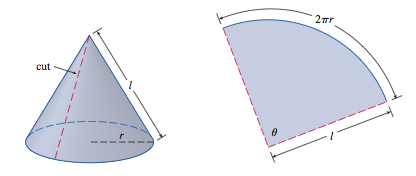
\includegraphics [scale=0.75] {cut_cone.png} \end{center}
The radius of that circle is the slant height of the cone, labeled $l$ in the figure.

\[ l = \sqrt{R^2 + H^2} \]
The total circumference of the circle flat in the plane would be $2 \pi l$.

However, the arc length along the sector that we actually used in the previous calculation is the circumference of the base of the cone, which is $2 \pi R$.

So the total area of the sector (equivalent to the surface area of the cone) is the total area of the circle, times the ratio of the sector circumference to the total circumference.
\[ S = \pi l^2 \ \frac{2 \pi R}{2 \pi l} = \pi Rl \]

The error in our application of calculus to this problem is a factor of $l/R$.

It turns out that what we did wrong is to multiply the circumference at each point by $dx$.  What we should have done is to multiply it by the little increment of slant instead.

Since 
\[ l = \sqrt{R^2 + H^2} \]

and in this problem
\[ R = H \]
\[ l = \sqrt{2} R \]

So the answer we obtained was $\pi R^2$, whereas the correct answer is $\pi R l$, and in this problem $l =  \sqrt{2} R$, so the correct answer is $\sqrt{2} \pi R^2$.

\section*{sphere:  surface area}
\subsection*{geometry}
Dunham has an analysis of Archimedes proof of what is called the hatbox theorem in this book \emph{The mathematical universe}.  I plan to add a section here based on his chapter, some day.

\subsection*{method: calculus}

Calculus provides a simple proof for the surface area, starting from the formula for the volume of a sphere
\[ V= \frac{4}{3} \pi R^3 \]

Suppose we take a sphere of radius $r$.  (I use $r$ here because for just this part, the radius will be a variable).  If we increase the radius by a little bit $dr$, then how does the volume change?  It changes exactly like the surface area!  That is
\[ dV = S \ dr \]
\[ S = \frac{d}{dr} \ V = \frac{d}{dr} \ \frac{4}{3} \pi r^3 = 4 \pi r^2 \]

Another way to see this is to break up the entire surface area of the sphere into small cones.  If the number of cones is very large, the base of each one is almost flat.  Call the area of the base $dS$ and the height is  of course $R$.  

The volume of a single cone is
\[ \frac{1}{3} R \ dS \]
If we add up the volumes of all the very thin cones from the entire sphere we will have the volume of the sphere
\[ \frac{1}{3}R \ S \]
but we already know this is just $4/3 \pi R^3$,
so clearly
\[ \frac{1}{3} R \cdot S = \frac{4}{3}\pi R^3 \]
\[ S = 4 \pi R^2 \]

\subsection*{slices}

Another approach is the method of slices, again.  We have a sphere of radius $R$ centered at the origin and we make slices perpendicular to the $x$ axis.  We have that 
\[ y = \sqrt{R^2 - x^2} \]
The circumference is then $2 \pi y$.

We need to be careful.  When we did the volume integral for a sphere in one dimension it was
\[ V = \int_{-R}^{R} \pi y^2 \ dx \]

Here we are looking for the surface area, and we are going to add up a bunch of small strips from the perimeter, but the differential is not $dx$  In other words, we can't just do
\[ S = \int  2 \pi y \ dx \]

For the surface area of a "volume of revolution", instead of $dx$ we need the actual length of the path element along the curve.  From Pythagoras we have 
\[ ds^2 = dx^2 + dy^2 \]
\[ = (1 + \frac{dy^2}{dx^2} ) \ dx^2 \]
\[ ds = \sqrt{1 + f'(x)^2} \cdot dx \]

What is the slope of a circle?
\[ y = \sqrt{R^2 - x^2} \]
\[ \frac{dy}{dx} = f'(x) = -\frac{x}{\sqrt{R^2 - x^2}}  = -\frac{x}{y}  \]
so
\[ ds = \sqrt{1 + f'(x)^2} \cdot dx \]
\[ = \sqrt{1 + \frac{x^2}{y^2}} \ dx \]

We want
\[ S = \int  2 \pi y \ ds \]
\[ = \int  2 \pi y \ \sqrt{1 + \frac{x^2}{y^2}} \ dx  \]
\[ = 2 \pi \int \sqrt{y^2 + x^2} \ dx \]
\[ = 2 \pi R \int \ dx \]
\[ = 2 \pi R \ x \ \bigg |_{-R}^R = 4 \pi R^2 \]

\subsection*{multivariable calculus}
I always have a hard time remembering how to work with surface integrals.  One helpful thing is that line integrals seem pretty straightforward to set up, though they are often an arithmetic mess.

The small element of the path is $ds$ so by Pythagoras we get 
\[ ds^2 = dx^2 + dy^2 \] 
and then a little rearrangement gives:
\[ ds^2 = \ [ \ 1 + (\frac{dy}{dx})^2 \ ] \ dx^2 \] 
\[ ds = \ [ \ \sqrt{1 + [f'(x)]^2} \ ] \ dx \]

The area element for surfaces is almost exactly the same:
\[ dS =  \sqrt{(1 + f_x)^2 + (f_y)^2} \  \cdot \ dA \]
So let's just remember the surface area element $dS$ as an extension of $ds$ to 3 dimensions.

With just this formula we can calculate something like the surface area of a sphere.  Write
\[ x^2 + y^2 + z^2 = a^2 \]
where $a$ is the constant radius.  Then
\[ z = f(x,y) = \sqrt{a^2 - x^2 - y^2} \]
\[ f_x = \frac{1}{2} \ \frac{-2x}{\sqrt{a^2 - x^2 - y^2}} = -\frac{x}{z} \]
or by implicit differentiation:
\[ z^2 = a^2 - x^2 - y^2 \]
\[ 2 z \ dz = - 2 x \ dx \]
and then we get the same thing as before.  Similarly $f_y = -y/z$.

Then use the formula.  Plugging in $f_x$ and $f_y$:
\[ dS = \ [ \ \sqrt{(\frac{x}{z})^2 + (\frac{y}{z})^2 + 1} \  ] \ dA \]
\[ = \frac{1}{z}  \ [ \ \sqrt{(x^2 + y^2 + z^2} \  ] \ dA \]
\[ dS = \frac{a}{z} \ dA \]

We want to set up $\int dS$, but it's pretty ugly in $x,y$.  We get
\[ \int_{-a}^a \int_{-\sqrt{a^2-x^2}}^{\sqrt{a^2-x^2}} \frac{a}{\sqrt{a^2 - x^2 -y^2}} \ dy \ dx \]
The inner integral is essentially:
\[ \int \frac{1}{\sqrt{c^2 -y^2}} \ dy \]
for the constant $c^2 = a^2 - x^2$, and we don't have $y$ so we need to do a trig substitution.  This comes out to be
\[ \sin^{-1} \frac{y}{c} \]
evaluated between $-c$ and $c$.  
\[ \sin^{-1} \frac{y}{c} \  \bigg |_{-c}^c = \frac{\pi}{2} - (- \frac{\pi}{2}) = \pi  \]
The outer integral is then
\[ \int_{-a}^a \pi a \ dx = 2 \pi a^2 \]

It is much nicer to switch to $r,\theta$.  We do this to check ourselves. Let
\[ x^2 + y^2 = r^2 \]
\[ z^2 = a^2 - x^2 - y^2 = a^2 - r^2 \]
\[ \int dS = \int_0^{2 \pi} \int_0^a  \frac{a}{\sqrt{a^2 - r^2}} \ r \ dr \ d \theta \]

The inner integral is essentially $1/\sqrt{u} \ du$
\[ \int \frac{1}{\sqrt{a^2 - r^2}} \ r \ dr = -\sqrt{a^2 - r^2}  \]
so we obtain
\[ a \ [ \ -\sqrt{a^2 - r^2} \ ] \ \bigg |_0^a = a^2 \]
which is zero at the upper bound and $-a^2$ at the lower bound.  Subtracting, we obtain $a^2$, and with the outer integral, the whole thing is $2 \pi a^2$.

We are a factor of $2$ off from the known result using both methods, and realize that when we wrote 
\[ z = f(x,y) = \sqrt{a^2 - x^2 - y^2} \]
we were only looking at the upper hemisphere, so a factor of $2$ is missing.

\chapter{Spherical cap}
Here is a figure from Wolfram for a spherical cap.  We are interested in formulas for the area and volume of the solid obtained by slicing through a sphere, where the height of the cap that is produced is $h$, and the distance of closest approach to the center of the sphere is $R-h$.
\begin{center} 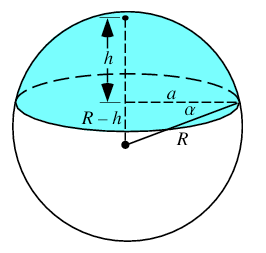
\includegraphics [scale=0.6] {spherical_cap.png} \end{center}

\subsection*{geometry}
If we start from the equator, and think about a thin belt going around the sphere, the belt has length equal to the circumference $2\pi R$ and width $h$, and thus area $S$:
\[ S = 2 \pi R h \]

We believe this should be the formula for the surface area of a belt of width $h$, at least near the equator.  In the figure, this width is labeled as $R-h$, because we are more interested in the cap.  Thus, for the calculation below, this area will be $2\pi R(R-h)$.

Consider that the total surface area of the hemisphere is $2\pi R^2$ so the area of the cap is the difference
\[ S = 2\pi R^2 -  2 \pi R (R-h) = 2 \pi Rh \]

That's a surprising result, that the area of the cap depends only on $R$ and its width (here called $h$).  At least, that is certainly true in the limit as the width of the belt at the equator is very small.

\subsection*{polar cap}
Furthermore, if we look in the figure at the right triangle with $h$ and $a$ as the sides, we can draw the hypotenuse of that triangle and call it $r$ (it's not actually labeled in the figure).  

It is sometimes called the slant height.  We calculate
\[ a^2 = R^2 - (R - h)^2 = 2 Rh - h^2 \]
\[ r^2 = a^2 + h^2 = 2 Rh - h^2 + h^2 = 2 Rh \]

Now think about a very small spherical cap, then it would be almost flat, a circle, and its radius would be $r$ and area
\[ S = \pi r^2 \]
But $r^2 = 2Rh$, so again we have the same formula for the surface area of a small cap and a belt near the equator!

\subsection*{generally}
Now consider a belt of width $h$ at some position which is not close to either the top or the equator of the sphere, but somewhere in the middle, in the temperate latitudes.

In using the formula $S = 2 \pi R h$, if $h$ is the width of the projection of the belt on the $z$-axis, that suggests that the circumference at this position is $2 \pi R$, which is obviously wrong.  It should be $2\pi a$.

What is going on is that the radius $a$ at the position of the cut is smaller than $R$ by a factor of $\cos \alpha$.  However, the slant height of the belt is larger than $h$ by the same factor.

The reason is that the tangent to the circle where we are performing the cut is perpendicular to $R$.  In the figure below, the angle that it forms with $a$ is the complement to $s$ (call it $t$) and the slant height is $h \sin t = h \cos s$.

\begin{center} 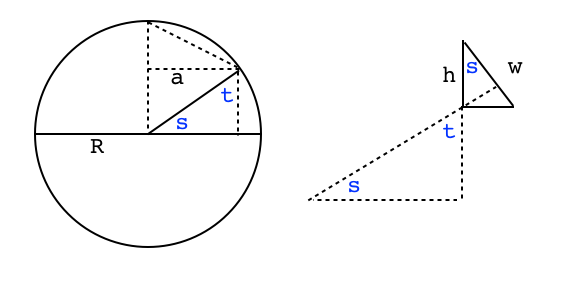
\includegraphics [scale=0.6] {sphcap2.png} \end{center}

We want the area of the spherical belt of height $h$  whose radius is $a$.  The angles are labeled in blue as $s$ and $t$, and they are complementary angles.
\[ a = R \cos s \]
So $a$ is smaller than R by the factor $\cos s$.  In the right panel, we see a small triangle at the surface of the sphere.  The width $w$ is flat on the surface, and since the dotted line is the radius $R$, $R$ makes a right angle where it intercepts $w$.  By complementary angles, we can see that the angle at the top of this triangle is also equal to $s$, so we have the relationship
\[ h = w \cos s \]
So the true area is
\[ 2 \pi a w = 2 \pi R \cos s \frac{h}{\cos s} = 2 \pi R h \]
The cosine of the angle comes in twice, and these factors cancel.  The formula $2\pi R h$ is correct everywhere.

\subsection*{calculus}
As we've seen, the surface area of a volume of revolution is
\[ S = 2 \pi \int y \sqrt{1 + (\frac{dy}{dx})^2} \ dx \]
The square root comes from the surface area element.  This formula looks unwieldy (and often is difficult to work with).  But in this particular case it simplifies dramatically.

If we take a circle as the curve, with formula
\[ x^2 + y^2 = R^2 \]
\[ 2x \ dx + 2y \ dy = 0 \]
\[ \frac{dy}{dx} = - \frac{x}{y} \]
So
\[ S = 2 \pi \int y \ \sqrt{1 + \frac{x^2}{y^2}} \ dx \]
\[ S = 2 \pi \int \sqrt{y^2 + x^2} \ dx \]
\[ S = 2 \pi \int R \ dx = 2 \pi R x \]
Evaluated between $x=a \to x=b$
\[ s = 2 \pi R (b-a) = 2 \pi R h \]

This makes it very clear that the area does not depend where we are on the sphere.  A spherical cap with height $h$ has the same area as a belt of width $h$ wrapped around the equator, or any belt of width $h$ in between the two.

And as we noticed before, the area of a belt or sperical cap, $2 \pi R h$, is equal to the surface area of a cylinder of radius $R$ and height $h$, the so-called hat-box theorem of Archimedes.
\begin{center} 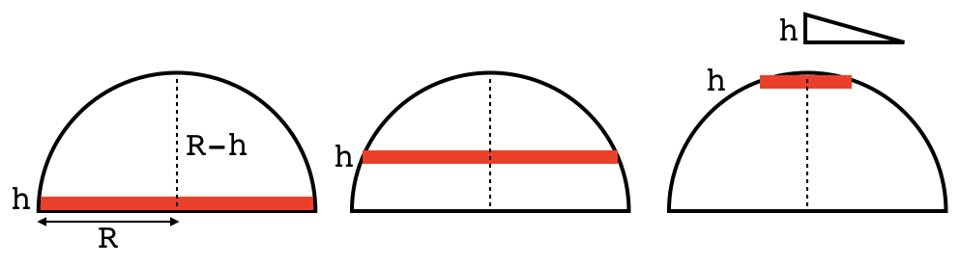
\includegraphics [scale=0.4] {hatbox.jpg} \end{center}

\section*{spherical cap:  volume}
\subsection*{calculus}
Here we will derive the formula for the volume of a spherical cap.  This is the solid obtained by slicing off a part of a sphere with a plane. 
\begin{center} 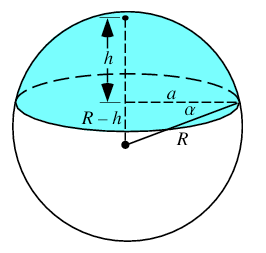
\includegraphics [scale=0.6] {spherical_cap.png} \end{center}
The formula is 
\[ V_{cap} = \frac{1}{3} \pi h^2(3R - h) \]
or equivalently
\[ V = \pi(Rh^2 - \frac{1}{3} h^3 )\]
We can see that this equation makes sense for the extreme case where $h=R$.  We get 

\[ V = \frac{1}{3} \pi R^2(3R - R) =   \frac{2}{3} \pi R^3 \]

One way to do spherical volumes is by integration of slices as shown in this figure (from Strang)
\begin{center} 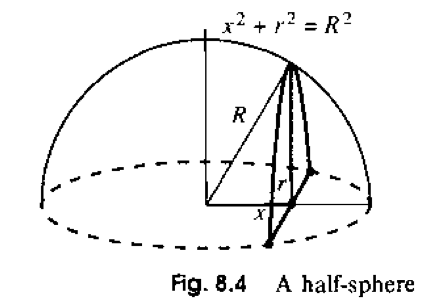
\includegraphics [scale=0.6] {sph_slices.png} \end{center}

This approach is basically the same as what I showed when we calculated the volume of the sphere using calculus, before.

In Strang's derivation, at each value of $x$, the hemisphere (of radius $R$) has a cross-section that is a half-circle with radius $r$ such that
\[ x^2 + r^2 = R^2 \]
the area of this hemisphere cross-section is
\[ A = \frac{1}{2} \pi r^2= \frac{1}{2} \pi (R^2 - x^2) \]
For the whole sphere, each cross-section is a circle with area
\[ A =  \pi r^2= \pi (R^2 - x^2) \]

For the volume, we just add up all these slices.  To make it simple, take $x$ from $0 \to R$ 
\[ V =  \pi \int_{0}^{R}  (R^2 - x^2) \ dx \]
\[ =  \pi \ [ \ R^2x - \frac{1}{3}x^3 \ ] \ \bigg |_{0}^R =  \frac{2}{3}\pi R^3 \]
Multiply by a factor of $2$ to get the whole thing.

The key insight is, we can get a spherical cap (or a belt), just by changing the lower limit of integration to $x=R-h$  !!  
\begin{center} 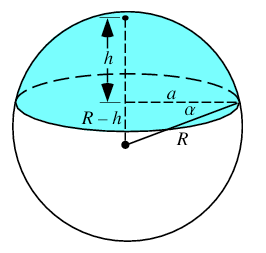
\includegraphics [scale=0.6] {spherical_cap.png} \end{center}
We need to evaluate
\[ V = \pi \ [ \ R^2x - \frac{1}{3}x^3 \ ] \ \bigg |_{R-h}^R \]
Leave aside the factor of $\pi$, and break the expression into two parts 
\[ R^2x  \ \bigg |_{R-h}^R - \frac{1}{3} x^3  \ \bigg |_{R-h}^R \]
For the left term we get
\[ R^3 - R^3 + R^2h = R^2h\]
For the right side we get
\[ -\frac{1}{3} R^3 + \frac{1}{3}(R-h)^3 ) \]
\[=  -\frac{1}{3} R^3 + \frac{1}{3} R^3 - R^2h + Rh^2 -\frac{1}{3} h^3 \]
Adding left and right terms together, the $R^2h$ terms cancel, and we have finally
\[ V = \pi (Rh^2 - \frac{1}{3} h^3) \]
Factoring out $h^2/3$
\[ V = \frac{1}{3} \pi h^2 (3R -h) \]
which is the formula we gave at the top.

We can calculate the volume of \emph{any} spherical belt by using the appropriate limits of integration.  For example, the belt from $r=0 \rightarrow r = R-h$ has volume
\[ V = \pi \ [ \ R^2x - \frac{1}{3}x^3 \ ] \ \bigg |_{0}^{R-h} \]
Leaving the $\pi$ aside for now
\[ R^2(R-h) - \frac{1}{3}(R-h)^3 \]
\[ R^3 - R^2h - \frac{1}{3}(R^3 - 3R^2h + 3Rh^2 - h^3) \]
\[ \frac{2}{3}R^3 - Rh^2 + \frac{1}{3} h^3  \]
With the factor of $\pi$
\[ V = \pi ( \frac{2}{3}R^3 - Rh^2 + \frac{1}{3} h^3 )  \]
Adding the cap and the belt together:
\[ V_{tot} =  \pi( Rh^2 - \frac{1}{3}h^3 + \frac{2}{3}R^3 - Rh^2 + \frac{1}{3} h^3) \]
Almost everything cancels
\[ V_{tot} =  \pi( \frac{2}{3}R^3) \]
The cap and the belt together make up a hemisphere.

\chapter{Apple core}
Another great problem I want to explore the use of polar coordinates to solve a problem of volume. This is the shape known as "the cored apple", shown in the figure (from Adams et al.).
\begin{center} 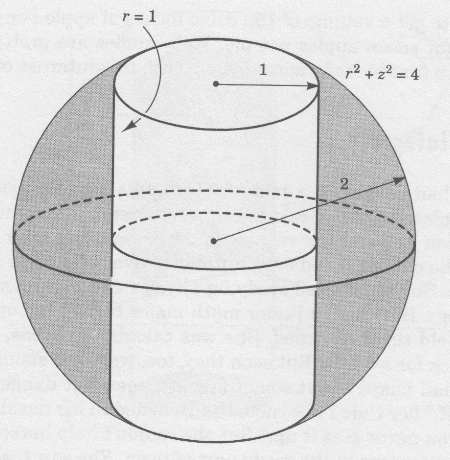
\includegraphics [scale=0.5] {apple_core.png} \end{center}

We have a sphere of radius $2$ which has had the central portion consisting of a cylinder plus the two spherical caps removed.

We are given that the cylinder has radius $1$.  The height $h$ is an unknown.  We need to find the volume of the part that remains.

\subsection*{geometry}

One way to do this problem is to find the volume of each spherical cap.  We worked this out in the previous chapter.  
\begin{center} \includegraphics [scale=0.6] {spherical_cap.png} \end{center}
If $h$ is the height of the cap, then its volume is
\[ V_{cap} = \frac{1}{3} \pi h^2(3R - h) \]

We are given the radius of the core, which is labeled $a$ in the second figure.  The equation we get using the Pythagorean theorem is
\[ (R - h)^2 + a^2 = R^2  \]
\[ R^2 - 2Rh + h^2 + a^2 = R^2 \]
We know that $R=2$ and $a=1$ so this simplifies to
\[ h^2 - 4h + 1 = 0 \]
Solve this using the quadratic formula to obtain:
\[ h = 2 \pm \ \sqrt{3} \]
Since $h$ cannot be greater than $R$ we take the negative square root:
\[ h = 2 - \sqrt{3} \]
\[ h^2 = 7 - 4 \sqrt{3} \]
We confirm that this value of $h$ solves the quadratic equation.

The volume of one spherical cap is
\[ V_{cap} = \frac{1}{3} \pi h^2(3R - h) \]
So 
\[ h^2(3R - h) = (7- 4 \sqrt{3})(6-(2-\sqrt{3})) \]
\[ = (7- 4 \sqrt{3})(4 + \sqrt{3})) \]
\[ = 28 - 12 + (-16 + 7) \sqrt{3} \]
\[ = 16 - 9 \sqrt{3} \]

We have two of these
\[ V = 2 \cdot \frac{\pi}{3} \cdot (16 - 9 \sqrt{3}) \]

The volume of the cylinder is the area of the cross-section
\[ \pi \cdot 1^2 = \pi \]
 times the height, which is $2(R-h) = 2 \sqrt{3}$.
\[ V = 2 \pi \sqrt{3} \]
We have to subtract both of these from the volume of the whole sphere, which is $32 \pi/3$.  The desired quantity is
\[ V = \frac{32 \pi}{3} - 2 \pi \sqrt{3} - \frac{2\pi}{3} \ (16 - 9 \sqrt{3}) \]
\[ = \pi \ [ \ \frac{32}{3} - 2 \sqrt{3} - \frac{2}{3} \ (16 - 9 \sqrt{3}) \ ] \]
\[ = \pi \ [ \ - 2 \sqrt{3} - \frac{2}{3} \ ( - 9 \sqrt{3}) \ ] \]
\[ = \pi \ [ \ 4 \sqrt{3}) \ ] \]
I get
\[ V = 21.77  \]
Just grind through it and we get there.

\subsection*{calculus}

There is a more elegant approach, using calculus.  Consider the sphere as a surface above the circle.  For the circle we have $x^2 + y^2 = r^2$, where now we are using $r$ as a \emph{variable} that could range from $0 \rightarrow R$.

In Cartesian coordinates the circle is
\[ x^2 + y^2 + z^2 = R^2 \]
Using polar coordinates for $x$ and $y$ we have 
\[ r^2 + z^2 = R^2 \]
\[ z = \sqrt{R^2 - r^2} = \sqrt{4 - r^2}  \]
We will do a double integral over the the $xy$-plane, adding up the value of this function for each small area element $dA$.  In polar coordinates, the area element is
\[ dA = r \ dr \ d \theta \]
so, for example, the basic area integral is
\[ A = \int dA = \int_{\theta=0}^{2 \pi} \int_{r=0}^R r \ dr \ d \theta = \int_{\theta=0}^{2 \pi} \frac{1}{2}R^2 \ d \theta = \pi R^2 \]

Now, what we want is to integrate the surface height over the whole area, plugging in from above we get
\[ V = \int dV = \int_{\theta=0}^{2 \pi} \int_{r=0}^R \sqrt{R^2 - r^2}  \ r \ dr \ d \theta \]
This integral is not hard to do because we have the derivative of what is under the square root sign.  Let $u = R^2 - r^2$.  Then
\[ du = -2r \ dr \]
\[ -\frac{1}{2} \ du = r dr \]
so the inner integral is
\[ \int -\frac{1}{2} \sqrt{u} \  du = -\frac{1}{3} u^{3/2} \]
Substituting back, the inner integral (for the whole sphere) is 
\[ -\frac{1}{3} (R^2 -r^2)^{3/2} \bigg{|}_0^R = \frac{1}{3}(R^2)^{3/2} =  \frac{1}{3} R^3 \]

When we do the outer integral we pick up an extra factor of $2\pi$, which gives the correct value for the volume of the hemisphere.
What is great about this approach is that we don't have to start at $r=0$.  This simplifies our problem enormously.  In the problem, we start from $r=1$ (and we have $R=2$).  So this gives the volume we seek as
\[ V = \int dV = \int_{\theta=0}^{2 \pi} \int_{r=1}^2 \sqrt{4 - r^2}  \ r dr d \theta \]
The inner integral is
\[ -\frac{1}{3} (4 -r^2)^{3/2} \bigg{|}_1^2 = \frac{1}{3}(3)^{3/2} =  \sqrt{3} \]
Now we have
\[ V =  \int_{\theta=0}^{2 \pi} \sqrt{3} \ d \theta \]
which is just $2\pi \sqrt{3}$.  Multiply by $2$ for the whole apple, we get $4 \pi \sqrt{3}$.  This matches what we had previously.

Adams, Thompson and Hass.  \emph{How to Ace the Rest of Calculus}

\chapter{Ellipse}
\section*{parametrization}
\begin{center} \includegraphics [scale=0.5] {ellipse_draw.png} \end{center}

Learning how to draw an ellipse using two pins and a circular piece of string holding a pencil is an early adventure in mathematics.  The ellipse is the set of all points whose combined distance to the two pins (foci) is the same.

\begin{center} \includegraphics [scale=0.5] {ellipse_wikipedia.png} \end{center}

The pin positions with respect to the origin or center are called the foci, lying at the points ($\pm f,0$).  The lengths of the axes (called semi-major and semi-minor) are usually labeled $a$ and $b$.  Consider the situation when the pencil is at the point $(0,a)$.  The length $L$ of the string is equal to twice the distance to the left focus, $L = 2(f+a)$, so

\[ a = \frac{L}{2} - f \]

We learn in algebra that the equation for an ellipse is
\[ \frac{x^2}{a^2} + \frac{y^2}{b^2} = 1 \]

Here are three ellipses drawn with the same center.

\begin{center} \includegraphics [scale=0.5] {ellipses_three.png} \end{center}

They were drawn by adjusting the value on the right-hand side of the equation

\[ \frac{x^2}{a^2} + \frac{y^2}{b^2} = r^2 \]

where $r = \{ 1/2,1,2 \}$.  This is equivalent to scaling both $a$ and $b$ by the same factor of $r$

\[ \frac{x^2}{(ra)^2} + \frac{y^2}{(rb)^2} = 1 \]

When $r=2$ we need to make the string a bit less than twice as long, because the length $f$ is also involved:

\[ ra = r(\frac{L}{2} - f) \]

\subsection*{parametrization}

An alternative view is the one below, which shows (black curves) the upper half of two circles of radius $r=1$ and $r=2$ and an ellipse whose equation is 
\[ \frac{x^2}{2^2} + \frac{y^2}{1} = 1 \]

\begin{center} \includegraphics [scale=0.5] {p_ellipse.png} \end{center}

Here $a=2$ and $b=1$.

The standard parametrization of the ellipse is
\[ x = a \cos t \]
\[ y = b \sin t \]
which I had trouble visualizing, until I drew the picture.  The point is that the parameter $t$ is \emph{not} the angle that a ray to $P$ makes with the $x$-axis, as it is for the circle.  Instead, to find the $x$ value of $P$ corresponding to $t$, we extend the ray with angle $t$ to the larger circle, with radius $a$, where we read off the $x$-value as 
\[ x=a \cos t \]
We go back to find the intersection of the same ray with the small circle to get 
\[ y = b \sin t \]

The algebraic way to do this is to show that the parametrization is equivalent to the original formulation
\[ x^2 = a^2 \cos^2 t \]
\[ y^2 = b^2 \sin^2 t \]
\[ \frac{x^2}{a^2} + \frac{y^2}{b^2} = \cos^2 t + \sin^2 t = 1 \]
as expected.

\subsection*{rotation}

Let's return to the diagram of the ellipse with two bounding circles of radius $a$ and radius $b$.  There is a new diagram on the next page.

Consider the coordinates of the point $P=(x,y)$ (the red dot in the first quadrant) as functions of the angle $t$.  As we said, $t$ is \emph{not} the angle of a ray from the origin to $P$.

Let's draw a ray (blue dotted line) from the origin that does have angle $t$ with the $x$-axis.  How to find $x$ and $y$ from the diagram.  For $x$, extend the ray to the outer circle.  The radius is $a$, the angle is $t$, and

\[ a \cos t = x \]

This is the parametrization of the ellipse introduced above.

\begin{center} \includegraphics [scale=0.5] {ellipse_fancy.png} \end{center}

The ray drawn with angle $t$ has the same $x$-intercept with the outer circle as our point $P$ on the ellipse.  Similarly, the intercept of the ray with the inner circle has the same $y$-value as the point $P$ on the ellipse.

We estimate the point $P=(1.2,0.8)=(6/5,4/5)$.  Using our algebraic equation:

\[ \frac{x^2}{a^2} + \frac{y^2}{b^2} = 1 \]

Recall that $a=2$ and $b=1$ so

\[ x^2 + 4y^2 = 4 \]

Plugging in for $x^2$ and $y^2$ we get

\[ \frac{36}{25} + 4 \ (\frac{16}{25}) = \frac{100}{25} = 4 \]

as expected.  Reading off the intercepts for the ray with angle $t$ (dotted blue line) with the outer circle, we have the point $(1.2,1.6)$ at a distance $2$ from the origin.  Thus,

\[ \frac{1.2}{2} = 0.6 = \cos t \]
\[ t \approx 0.927\ \text{rad} \approx 53^{\circ} \]

Looking again at the figure, we want to consider what happens for the angle $u = t + \pi/2$.  This is the dotted blue ray in the second quadrant.

We might calculate the values of sine and cosine for $u$, but notice that if we view $u$ as a vector, its \emph{dot product} with $t$ must be equal to zero.  The coordinates of the intercept of the rotated vector with the outer circle are $(-1.6,1.2)$, so the cosine of the angle $u$ is

\[ \cos u = -0.8 \]
\[ u \approx 2.498 = t + \frac{\pi}{2} \ \text{rad} \approx 143^{\circ} \]

We confirm that 

\[ 2.498 - 0.927 = 1.57 = \frac{\pi}{2} \]

The coordinates of the point on the ellipse are $(-1.6,0.6)$, which we check against the formula

\[ x^2 + 4y^2 = 4 \]
\[ (1.6)^2 + 4(0.6)^2 = 2.56 + 4(0.36) = 4 \]

(no clean fractions this for this one).

\subsection*{tangent}

Finally, and this is really the point of the write-up, the vector to the point, call it $Q$, on the ellipse (red dot in the second quadrant) is the tangent to the ellipse for the point $P$ in the first quadrant, and vice-versa.

How did this happen?  Recall what we did.  We had 

\[ x = a \cos t \]
\[ y = b \sin t \]

The rotated point $Q = (x',y')$ is

\[ x' = a \cos (t + \frac{\pi}{2}) \]
\[ y' = b \sin (t + \frac{\pi}{2}) \]

\begin{center} \includegraphics [scale=0.75] {sine_cosine_wikipedia.png} \end{center}

Sine is like cosine, but shifted to the right by $\pi/2$

\[ \cos \theta = \sin (\theta + \frac{\pi}{2}) \]
\[ \sin \theta = - \cos (\theta + \frac{\pi}{2}) \]

So

\[ x' = a \cos (t + \frac{\pi}{2}) = -a \sin t \]
\[ y' = b \sin (t + \frac{\pi}{2}) = b \cos t \]

So what, you say.  Well, let's look at the position vector, which can be written $\mathbf{r}(t)$, since it's a function of the angle $t$ or the time, but we will just use $\mathbf{r}$.  It has components $x$ and $y$.

\[ \mathbf{r} = \ \langle x,y \rangle \ = \ \langle a \cos t,b \sin t \rangle \ \]

Now, the tangent to the ellipse is precisely the direction in which a particle at $(x,y)$ is currently moving on the ellipse.  The tangent vector points in the same direction as the velocity vector, but $\mathbf{v}$ is just the time-derivative of the position vector.

\[ \mathbf{v} = \frac{d\mathbf{r}}{dt} = \ \langle \frac{dx}{dt}, \frac{dy}{dt} \rangle \ = \ \langle -a \sin t,b \cos t \rangle = \ \langle x',y' \rangle \]

And that's the point.   :)

\section*{area}
The area of an ellipse can be computed in several different ways, all interesting.  The simplest way is rescaling.  In $xy$-coordinates, the formula is
\[ \frac{x^2}{a^2} + \frac{y^2}{b^2} = 1 \]
\[ (\frac{bx}{a})^2 + y^2 = b^2 \]
What this says is that if the $x$ value of each point on the ellipse is re-scaled by a factor of $b/a$, the result is
\[ u = \frac{b}{a}x \]
\[ u^2 + y^2 = b^2 \]
a circle of radius $b$ and area $A = \pi b^2$.  Because the scaling factor is only in the $x$-direction
\[ x = \frac{a}{b}u \]
the area of the original ellipse is bigger by a factor of $a/b$
\[ A = \pi b^2 \ \frac{a}{b} = \pi ab \]
We might also argue as follows.  The area of the ellipse clearly depends on both $a$ and $b$, so we write
\[ A = k a b \]
where $k$ is an unknown constant.  Now, if $a=b$, we obtain
\[ A = k a^2 \]
but this is just a circle, with known area
\[ A = \pi a^2 = k a^2 \]
Hence $k = \pi$ and $A = \pi ab$.

\subsection*{single variable calculus}
Solve the equation of the ellipse for $y$
\[ y = b \sqrt{1 - \frac{x^2}{a^2} } \ dx  \]
We take the positive square root, and integrate from $x = 0 \rightarrow a$, and should obtain $1/4$ the area of the ellipse.
\[ A = 4 b \int \sqrt{1 - \frac{x^2}{a^2} }  \]
The first thing to do is to get rid of the $a$ by substitution.  Let $u = x/a$, so $au = x$ and $a \ du = dx$, then
\[ A = 4 ab \int \sqrt{1 - u^2} \ du  \]
The next step is to recognize that $f(x) = \sqrt{1-u^2}$ is the equation of a circle.  Since we are integrating over the first quadrant, the value of the area is just $\pi/4$.  The whole thing is $\pi$ and we pick up the factor $ab$ from outside to give $A = \pi ab$.

If you failed to see this, you can do a trig substitution.  If $u$ is the side opposite angle $\theta$, and $1$ is the hypotenuse, then 
\[ \sqrt{1-u^2} = \cos \theta \]
\[ u = \sin \theta \]
\[ du = \cos \theta \ \ d\theta \]
and the integral becomes
\[ 4 ab \int \cos^2 \theta \ d\theta  \]
Before we do the integration, consider the changing bounds.  We originally had $x = 0 \rightarrow a$, in changing to $u$ by remembering that
\[ au = x \]
we obtain $u = 0 \rightarrow 1$.  Then, in changing to $\theta$ we have
\[ u = \sin \theta \]
\[ \theta = \sin^{-1} u \]
and we have $\theta = 0 \rightarrow 2\pi$.
I'm not going to do the integral here, but just give the result
\[ \int \cos^2 \theta \ d \theta = \frac{1}{2} (\theta + \sin \theta \cos \theta) \]
(and there are other ways to write it).  But we will take a moment to check that by differentiating
\[ \frac{d}{d \theta} \ \frac{1}{2} (\theta + \sin \theta \cos \theta) \]
\[ =  \frac{1}{2}(1 + \cos^2 \theta - \sin^2 \theta) \]
\[ =  \frac{1}{2}(1 + \cos^2 \theta + \cos^2 \theta - 1) = \cos^2 \theta \]

So we need to evaluate
\[ 4ab \ [ \ \frac{1}{2} (\theta + \sin \theta \cos \theta) \ ] \ \bigg |_0^{\pi/2} \]
Only one term is non-zero and that is $\theta = \pi/2$ at the upper limit.  We obtain
\[ A = 4ab \ (\frac{1}{2}\ \frac{\pi}{2}) = \pi ab \]

\subsection*{Green's Theorem}
State the theorem:
\[ \oint_C \mathbf{F} \cdot \mathbf{r} = \iint_R \nabla \times \mathbf{F} \ dA \]
\[ \int_C M \ dx + N \ dy = \iint_R (N_x - M_y) \ dx \ dy \]
The theorem equates the line integral around a closed path with an area over a region.

To start with, if $\mathbf{F}$ is the gradient of some function, we call such a function the potential, and the integral of the work over a closed path is just zero.

Of course, my favorite example is the area of the ellipse.  

Suppose $N_x - M_y = 1$.  Then the curl integral is the area of the region.  An example would be if $\mathbf{F} = \ \langle M,N \rangle \ = \ \langle -y/2,x/2 \rangle$.  Parametrize the ellipse.
\[ x = a \cos \theta \]
\[ y = b \sin \theta \]
So, for the left hand side we have
\[ \int_C M \ dx + N \ dy = \int_C -\frac{1}{2}y \ dx + \frac{1}{2}x \ dy \]
\[ = \int_0^{2\pi} (-\frac{1}{2})(b \sin \theta) \ (-a \sin \theta) \ d \theta \ + (\frac{1}{2})(a \cos \theta) \ (b \cos \theta) \ d\theta \]
\[ = \int_0^{2\pi} (\frac{ab}{2}\sin^2 \theta + \frac{ab}{2}\cos^2 \theta) \ d \theta = \frac{ab}{2} \int_0^{2\pi} \ d \theta = \pi a b\]

\section*{volume}

\begin{center} \includegraphics [scale=0.5] {ellipse_wikipedia.png} \end{center}

I want to compute the volume of an ellipsoid.  We imagine the solid formed by rotating the ellipse around the $x$-axis.  For each value of $x$, this solid will have a cross-section whose radius is equal to $y$, so to get the volume of the ellipse we do

\[ V = \int_{-a}^{a} \pi y^2 dx \]

Now, 
\[ x = a \cos t \]
\[ dx = -a \sin t \ dt \]
And we will have to find new limits for the integral.  Let's set it up first
So
\[ V = \pi \int (b^2 \sin^2 t)(-a \sin t) \ dt\]
Previously we had 
\[ x = -a \rightarrow a \]
The lower limit corresponds to $t = \pi$ and the upper limit to $t=0$.
\[ V = \pi a b^2 \int_{\pi}^{0} (\sin^2 t) (- \sin t) \ dt\]
\[ = \pi a b^2 \int_{\pi}^{0} (1 - \cos^2 t) (- \sin t) \ dt\]
\[ = \pi a b^2 \ [ \ \cos t - \frac{1}{3} cos^3 t \ ] \ \bigg |_{\pi}^{0} \]
\[ = \pi a b^2 \ [ \ (1 - \frac{1}{3}) - (-1 + \frac{1}{3})   \ ] \  \]
\[ = \frac{4}{3} \pi a b^2  \]

This is quite beautiful.  If we consider the three axes in space, for $y$ and $z$ the surface passes through at $b$, so $b$ counts twice in the volume.  If we rotated the other way (around the $y$ axis), we would obtain $\frac{4}{3} \pi a^2 b$.

\chapter{Paraboloid}
\section*{volume}

A paraboloid is a solid whose vertical cross-section is a parabola (often, it is oriented along the $z$-axis).  It may open up, or down.  The cross-sections parallel to the $xy$-plane are typically circles, though the shape factors for the parabolas in the $xz$- and $yz$-planes could be different, leading to an ellipse for the cross-sections.

Consider
\[ z = 2 - x^2 - y^2 \]

This is a paraboloid that opens down ($z$ gets large and negative when either $x$ or $y$ get large).  The vertex is at $z=2$.  When $z=0$, the cross-section is a circle

\[ x^2 + y^2 = 2 \]

 of radius $r=\sqrt{2}$.

Usually, cylindrical coordinates are good for dealing with this solid.  For example, in those coordinates, the surface area element is $dS = r \ dz \ d \theta$.

But let's start with a method from 1-D calculus.  Suppose we turn the paraboloid so that its symmetry axis is the $x$-axis, and its vertex is at the origin.  We can model this as being generated by revolution of the graph of $f(x) = \sqrt{x}$ around the $x$-axis.

The general formulation is that at each point $x$, we have a circle of radius $f(x)$ and area $\pi f(x)^2$.

Here, $f(x)=\sqrt{x}$, and area $A = \pi r^2 = \pi x$.  If we consider the width of each slice to be $dx$, then for the volume just add all these up

\[ V(x) = \int A(x) \ dx = \int \pi x \ dx \]
\[ = \frac{\pi}{2} \ x^2 \ \bigg |_a^b \]

For the unit paraboloid at $b=1$, we get $\pi/2$.  And our first paraboloid ($b=2$) has a volume of 

\[ V = 2 \pi \]

Now, consider the shape factor for the parabola, $a$.  In the standard equation $y=ax^2$, and the larger $a$ is, the faster the parabola grows in the $y$-direction.  But here, we have the parabola "opening" in the $+x$-direction.  That is, we have $x = a y^2$ and so $y= \sqrt{x/a}$.  Thus

\[ V(x) = \int A(x) \ dx = \pi \int \frac{x}{a} \ dx =  \frac{\pi}{a} \int x \ dx \]

and we have a factor of $1/a$ for the final volume.  

We can ask in another way if these formulas make sense.  Consider the parabola $y=x^2$ in the unit square.  The area "under" the curve is $1/3$, which is another way of saying that the area "over" the curve and inside the parabola is $2/3$.  Compare with the circle, whose area over the unit square is $\pi/4 \approx 3/4$.  The circle is a bit "fatter" than the parabola and we expect its volume, when we do the rotation, to be larger in proportion.  So this looks reasonable.

\subsection*{another method}

I want to find the volume using cylindrical coordinates.  I'd also like to generalize the problem.  In 1D we orient the vertex at the origin and integrate (usually) from $0 \rightarrow b$.  When we turn the volume so that it aligns with the $z$-axis, we usually place it with the bottom of the desired region in the $xy$-plane.  So I'm going to re-write the equation as

\[ z = f(x,y) = c - x^2 - y^2 \]

where c is the height of the parabola we are measuring.  

We are going to use $r, \theta, z$.  So we need to find the limits on $r$.  The "shadow" of the paraboloid is a circle in the $x,y$-plane 

\[ z = 0 = c - x^2 - y^2 \]
\[ x^2 + y^2 = r^2 = c \]
\[ r = \sqrt{c} \]

The volume in cylindrical coordinates is
\[ V = \iiint dV = \iiint r \ dz \ dr \ d \theta \]

What are the bounds on $z$?  Remember, if we integrate first with respect to $z$ then $r$ is \emph{fixed}.  For a given $r$

\[ z =  c - r^2  \]

So, the bounds on $z$ are $z=0 \rightarrow c - r^2$, and the inner integral is just
\[ \int_0^{c-r^2} r \ dz = r( c-r^2) \]

This gives us what we would have if we just started by thinking about the double integral of $f(x,y)$ or $f(r,\theta)$ over the region $R$ in the plane.

\[ V = \iint f(x,y) \ dx \ dy = \iint f(r,\theta) \ r \ dr \ d \theta \]

The middle integral is

\[ \int_0^{\sqrt{c}} cr - r^3 \ dr \]
\[ = \frac{1}{2}cr^2 - \frac{1}{4}r^4 \ \bigg |_0^{\sqrt{c}} \]
\[ = \frac{1}{2}c^2 - \frac{1}{4}c^2 =  \frac{1}{4}c^2 \]

times $2 \pi$ from the outer integral.  Hence $V= \pi/2 \cdot c^2$.

The way we've set up this problem, the region that we want starts at the $xy$-plane.  So there's not much point in preserving the option of starting evaluation of the middle integral at $a \ne 0$.  But if you did decide to do this you could.  Just remember to go back and fix the lower bound on $z$ in the inner integral.  That would also have to change.

\subsection*{double paraboloid}

\begin{center} \includegraphics [scale=0.4] {doubleparab.png} \end{center}

Just for fun, let's try to do a double paraboloid.  In the figure, the paraboloid that opens up is $z= x^2 + y^2$ while the one that opens down is $z = 1-x^2 - y^2$.  To match what we had in the earlier section, I'm going to change the upper one to be $z = 2-x^2 - y^2$.

We will use cylindrical coordinates to integrate.  The key to the problem, as usual, is to find the limits for $r$ and $z$.  First, solve for the intersection of the two surfaces:

\[ z = 2-x^2 - y^2 = x^2 + y^2 \]
\[ x^2 + y^2 = 1 = r^2 \]

So $r = 0 \rightarrow 1$.  Easy enough.  And $z$ ranges from the lower surface to the upper one.  Our integral is

\[ V = \int_0^{2\pi} \int_0^1 \int_{r^2}^{2-r^2} \ dz \ r \ dr \ d \theta \]

The middle integral is

\[ \int_0^1 2 - 2r^2 \ r \ dr  \]
\[ = 2\ (\frac{r^2}{2} - \frac{r^4}{4}) \ \bigg |_0^1 \]
\[ = 2 \cdot \frac{1}{4} = \frac{1}{2} \]

Multiply by $2\pi$ from the outer integral and that gives simply, $\pi$.  Notice that we have a duplicated version of the first volume, for which we found the answer $\pi/2$.  It checks.

\subsection*{paraboloid:  surface area}

Let's do the surface area paraboloid as well.  We can write the equation as
\[ z =  c - x^2 - y^2 \]
This one opens down, and the vertex is at $z = c$.

Suppose the sign of the $c$ term is positive and we want the area above the $xy$-plane.  In the plane, $z = 0$ so
\[ x^2 + y^2 = r^2 = c \]
The radius of the circle in the plane is $\sqrt{c}$.  That will be the upper bound of the radial integral in polar coordinates.

Recall our formula
\[ dS = \ [ \ \sqrt{(f_x)^2 + (f_y)^2 + 1} \  ] \ dA \]
Here $f_x = -2x$ and $f_y = -2y$ so
\[ dS = \ [ \ \sqrt{(f_x)^2 + (f_y)^2 + 1} \  ] \ dA \]
\[ S = \int dS = \int \sqrt{1 + 4x^2 + 4y^2} \ dA \]
This is, naturally, easier in polar coordinates.  $x^2 + y^2 = r^2$ so
\[ = \int_0^{2 \pi} \int_0^{\sqrt{c}} \sqrt{1 + 4r^2} \ r \ dr \ d \theta \]

The inner integral is
\[ = \frac{1}{12} \ (1 + 4r^2)^{3/2} \ \bigg |_0^{\sqrt{c}} \]
\[ = \frac{1}{12} \ [ \ (1 + 4c)^{3/2} - 1 \ ] \ \]
Multiply by $2 \pi$ to get the whole thing.

A value for $c$ that gives a nice result is $c = 2$, then
\[ S = 2 \pi \ \frac{1}{12} \ [ \ (1 + 4c)^{3/2} - 1 \ ] \ \]
\[ = 2 \pi \ \frac{1}{12} \ (27 - 1) = \frac{26}{6} \pi \]
which you can check (as we have before) by computing this as a volume of revolution.
\subsection*{normal vector}
In vector calculus, usually we are dealing with a field, and taking the dot product with $\mathbf{\hat{n}} \ dS$.

With a plane we get the normal vector as part of the equation.  For any other surface we recognize that, if $x$ changes by $1$ and $y$ doesn't change, then $z$ will change by $f_x$. 

It follows that one tangent vector to the surface is $\mathbf{u} = \langle 1, 0, f_x \rangle$ and another one is $\mathbf{v} = \langle 0, 1, f_y \rangle$.  The normal vector is any multiple of the dot product $\mathbf{u} \times \mathbf{v}$:
\[ \mathbf{N} =  \langle - f_x, - f_y, 1 \rangle \]

The length of $\mathbf{N}$ is the same factor we had above 
\[ \sqrt{(f_x)^2 + (f_y)^2 + 1} = | \mathbf{u} \times \mathbf{v} | \]
Therefore, when we multiply the unit normal vector (which is divided by this factor) and $dS$, which contains the same factor, we obtain a simplification
\[ \mathbf{\hat{n}} \ dS =  \langle - f_x, - f_y, 1 \rangle \ dA \]
So that's another one to just memorize.

\chapter{Stovepipe}
I came across an interesting problem in a chapter of Strogatz's \emph{The Joy Of x}.  He calls it the stovepipe problem.  We want to find the volume of the region formed from the intersection of two cylinders (of equal radius), that meet at right angles.

\begin{center} \includegraphics [scale=0.5] {stovepipe1.png} \end{center}

I really couldn't visualize it, but he told me that the horizontal cross sections of this solid are squares, and gave a picture.

\begin{center} \includegraphics [scale=0.5] {stovepipe2.png} \end{center}

and it makes sense, if you imagine cutting through a potato with a cylindrical bore, then repeating at right angles.  At each level, the side is formed by cutting along the edge of the cylinder, hence the opposite sides are parallel.  And since the two cuts use the same cylinder, all $4$ sides at any particular height are equal, giving a square.

So our problem is to find the length of the side at each value of the height.  We deal with the upper half of the solid, for simplicity.  If you draw a sketch of the vertical cross-section, at each distance $h$ from the base of the solid, extending up, the remainder of the height down to the base is $R-h$, and the half-length of the side is $s/2 = \sqrt{R^2 - h^2}$.

The volume is obtained by adding up all these slices

\[ V = \int_0^R 2  \sqrt{R^2 -h^2} \ dh \]

Let's simplify the problem further (for the moment) by dealing with the case where $R=1$  We need the integral

\[ \int \sqrt{1-h^2} \ dh \]

I certainly didn't know that off the top of my head.

\section*{a new integral}

You know that the derivative of the inverse sine is:
\[ \frac{d}{dx} \sin^{-1} x  = \frac{1}{\sqrt{1-x^2}} \]

(The way we get this:  let $x = x/1 = \sin t$, then $t = \sin^{-1} x$ and $\sqrt{1-x^2} = \cos t$ and
\[ \frac{dx}{dt} = \cos t = \sqrt{1-x^2} \]
\[ \frac{dt}{dx} = \frac{1}{\cos t} = \frac{1}{\sqrt{1-x^2}} \] 

Now, how about 

\[ \int \sqrt{1-x^2} \ dx \]

It's the same term, but it's on top rather than in the denominator.  What happens if we multiply top and bottom by $\sqrt{1-x^2}$?

\[ = \int \frac{1-x^2}{\sqrt{1-x^2}} \ dx \]
\[ = \int \frac{1}{\sqrt{1-x^2}} \ dx + \int \frac{-x^2}{\sqrt{1-x^2}} \ dx \]

Is this progress?  Now we have an extra power of $x$ in the term on the right.  Since we know we can integrate the square root using one power of $x$, and taking the derivative of the remaining factor of $x$ will make it go away, it sounds like we should try integration by parts

\[ \int u \ dv = uv - \int v \ du \]

Let $x = u$, then $dx = du$.  And let $-x/\sqrt{1-x^2} \ dx$ = $dv$.  Then
\[ v = \sqrt{1-x^2} \]

So the integral of this part is

\[ \int \frac{-x^2}{\sqrt{1-x^2}} \ dx = x \sqrt{1-x^2} - \int  \sqrt{1-x^2} \ dx  \]

We still can't integrate the term on the right, but now, we have two of them!  Putting it all together:

\[  \int \sqrt{1-x^2} \ dx = \int \frac{1}{\sqrt{1-x^2}} \ dx + x \sqrt{1-x^2} - \int \sqrt{1-x^2} \ dx  \]

So

\[ 2 \int \sqrt{1-x^2} \ dx =   \sin^{-1} x + x \sqrt{1-x^2} \]
\[ \int \sqrt{1-x^2} \ dx = \frac{1}{2}  \sin^{-1} x + \frac{x}{2} \sqrt{1-x^2}  \]

One more thing.  Suppose we have

\[ \int \sqrt{a^2-x^2} \ dx \]

We can pull out the $a$ as follows

\[ = a \int \sqrt{1- (\frac{x}{a})^2} \ dx \]

Let $u = x/a$, then $a \ du = dx$ and we have

\[ = a^2 \int \sqrt{1- u^2} \ du \]

So the final answer is

\[ \int \sqrt{a^2-x^2} \ dx = \frac{a^2}{2} \ [ \ \sin^{-1} \frac{x}{a} + \frac{x}{a} \sqrt{1-(\frac{x}{a})^2} \ ] \]

which can be rearranged slightly

\[ = \frac{a^2}{2} \ \sin^{-1} \frac{x}{a} + \frac{x}{2} \sqrt{a^2-x^2}  \]

I'll leave it to you to figure out the whole volume for the general case with radius $R$.

\chapter{Torus}

The general theory which allows us to calculate surface areas includes a formula for parametrized surfaces.  

For parametrization of a line or a curve we need only one variable.
\[ x = \cos t \ \ \ \  y = \sin t \ \ \ \ z = ct \]
where $t$ is the parameter and $c$ is a constant, is the parametrization of a helix.

For a surface (like a sphere, or a torus), we will need two parameters, which are usually called $u$ and $v$. 
\begin{center} \includegraphics [scale=0.4] {torus.png} \end{center}
To get the surface area, we will just calculate 
\[ V = \int \ du \ dv \]
over the appropriate range of the two variables.  There is an additional constant:  we need to figure out the exchange rate for the surface area element $dS$  (composed of sides $du$ and $dv$) to units of $dA$ (composed of $dx$ and $dy$).  More about that later.

A torus is like a small circle moved around in a larger circle.  The small circle is the cross-section of the donut (radius $r$), while the large circle traces out the path of the donut (radius $R$).  Our parameters will be the angles $\theta$ and $\phi$.  $\theta$ describes the position of on the large circle (the position of the center of the small circle) as 
\[ x_c = R \cos \theta \ \ \ \  y_c = R \sin \theta \]
In this approach, the donut's axis of symmetry is the $z$-axis, and the body of the donut is centered half above the $xy$-plane and half below it.  The second angle, $\phi$, describes where we are on the small circle.  In particular, the distance above or below the $xy$-plane will be
\[ z = r \sin \phi \]
The only tricky part is the finaly adjustment to obtain the actual $x$ and $y$ coordinates.  For $x$, when $\phi = 0$, we go out from the origin an additional distance $r$, while when $\phi = \pi$, we subtract the same distance.  Our first attempt is:
\[ x = x_c + r \cos \phi \]
\[ = R \cos \theta + r \cos \phi \]
While this is correct for $\theta = 0$ it is not correct for other angles.  We need an additional factor of
$\cos \theta$:
\[ x = R \cos \theta + r \cos \phi \cos \theta \]
\[ = \cos \theta (R + r \cos \phi) \]
It may not be clear that this works for all angles, but if $\theta = \pi/2$ we add nothing additional to $x_c$, and that is just what we want.  Similarly for $y$
\[ y = y_c + r \cos \phi \sin \theta \]
\[ = \sin \theta (R  + r \cos \phi) \]

Now, according to the theory, what we need to do is take the partial derivatives of these functions with respect to $\theta$ and $\phi$.  For example:
\[ x_{\theta} = \frac{dx}{d \theta} = \frac{d}{d \theta} \ \cos \theta (R + r \cos \phi) \]
We find that
\[ x = \cos \theta (R + r \cos \phi) \]
\[ x_{\theta} = -\sin \theta (R + r \cos \phi) \]
\[ x_{\phi} = -\cos \theta \ r \sin \phi \]
while
\[ y = \sin \theta (R  + r \cos \phi) \]
\[ y_{\theta} = \cos \theta (R + r \cos \phi) \]
\[ y_{\phi} = -\sin \theta \ r \sin \phi \]
$z$ does not depend on $\theta$ so
\[ z_{\theta} = 0 \]
\[ z_{\phi} = r \cos \phi \]
The position vector to a point on the surface is
\[ \mathbf{r} = \ \langle x,y,z \rangle \]
\[ \mathbf{r_{\theta}} = \ \langle x_{\theta},y_{\theta},z_{\theta} \rangle \]
\[ \mathbf{r_{\phi}} = \ \langle x_{\phi},y_{\phi},z_{\phi} \rangle \]

The unit for conversion is called the Jacobian.  It is the length of the vector $\mathbf{r_{\theta}} \times \mathbf{r_{\phi}}$.  It's a bit complicated, so let's do the pieces individually.  The vector product has three terms
\[ \hat{\mathbf{i}} \ y_{\theta} z_{\phi} -  y_{\phi} z_{\theta} \]
\[ = \hat{\mathbf{i}} \  \cos \theta (R + r \cos \phi) r \cos \phi - 0 \]
\[ \hat{\mathbf{j}} \ x_{\phi} z_{\theta} -  x_{\theta} z_{\phi} \]
\[ = \hat{\mathbf{j}} \  0 - \sin \theta (R + r \cos \phi) r \cos \phi  \]
The third term is most complicated
\[ \hat{\mathbf{k}} \ x_{\theta} y_{\phi} -  x_{\phi} y_{\theta} \]
\[ = \hat{\mathbf{k}} \sin \theta (R + r \cos \phi) \sin \theta \ r \sin \phi + \cos \theta \ r \sin \phi \cos \theta (R + r \cos \phi) \]
But notice that we have the same term times $\sin^2 \theta$ and $\cos^2 \theta$ so this reduces immediately to 
\[ = \hat{\mathbf{k}}  (R + r \cos \phi) \ r \sin \phi \]

The next (and nearly the last) step is to calculate the length of this vector, by squaring each term and adding.  Before we do that, notice that all three components contain a factor of $r (R + r \cos \phi)$.  We will leave that aside and remember it at the end.  The rest of the sum of squares is:
\[ \cos^2 \theta \cos^2 \phi + \sin^2 \theta \cos^2 \phi + \sin^2 \phi   \]
\[ = \cos^2 \phi + \sin^2 \phi  = 1 \]
So the factor we held aside is all that's left
\[ |\mathbf{r_{\theta}} \times \mathbf{r_{\phi}} | = r (R + r \cos \phi) \]

And the surface integral is just
\[ A_S = \int dS = \int_{\theta = 0}^{2 \pi} \int_{\phi = 0}^{2 \pi} |\mathbf{r_{\theta}} \times \mathbf{r_{\phi}}| \ d \phi \ d \theta \]
\[ = \int_{\theta = 0}^{2 \pi} \int_{\phi = 0}^{2 \pi} r (R + r \cos \phi) \ d \phi \ d \theta \]

Since $\theta$ is independent of $\phi$ and $R$ and $r$, we get
\[ = 2 \pi r  \int_{\phi = 0}^{2 \pi} (R + r \cos \phi) \ d \phi  \]
But the integral of $\cos \phi$ is just $\sin \phi$, which is zero at the upper and lower bounds on $\phi$, hence 
\[ = 2 \pi r  \int_{\phi = 0}^{2 \pi} R \ d \phi  \]
\[ = 2 \pi r  \ 2 \pi R \]
Which is pretty amazing.  We go around the torus along what is called its centroid, traveling a distance $ 2 \pi R$.  At each point we have the circumference of the small circle, which is $ 2 \pi r$.  

It seems strange that the curvature doesn't make any difference.  There is a theorem in geometry (the Theorem of Pappus), with the same result.  

Pappus also allows us to calculate the volume as
\[ V = \pi r^2 \ 2 \pi R \]

\chapter{Pappus Theorem}
Pappus' centroid theorem is actually a pair theorems about certain kinds of solids, called solids of revolution, where a curve $C$ is revolved around a central axis.  The two theorems relate to the surface area and volume.  There is a nice article about it at Mathworld
\vspace{2 mm}

\url{http://mathworld.wolfram.com/PappussCentroidTheorem.html}
\vspace{2 mm}

The first theorem states that the surface area $A$ is the product of the arc length $s$ of curve $C$ times the distance $d$ traveled by the geometric centroid of $C$.

The example in the wikipedia article is a torus of minor radius $r$ and major radius $R$.  Then the curve is a circle of radius $r$, the centroid of the curve is its center, and this point moves around a circle of radius $R$ the distance $2\pi R$.  The first term is the circumference $C$ of the curve (the small circle) and the total is

\[ A = 2 \pi r \ 2 \pi R = 4 \pi^2 r R \]

The second theorem depends on the area enclosed by the curve (and the y-axis).  The volume of this solid is the product of the area times the distance d traveled by the geometric centroid of this area (not the curve), which is here the same as before.

\[ V = \pi r^2 \ 2 \pi R = 2 \pi^2 R r^2 \]

Part of the trick here is going to be actually finding the geometric centroids.  

\subsection*{Cylinder}
Our first example is the cylinder, and here it's easy.  We revolve a parallel line segment around the y-axis.  The curve has length $H$.  

The centroid of the parallel line segment (the average distance of each point on the curve from the x-axis) is just the radial distance R, since all the points are the same distance away.  In addition, the centroid is also halfway along the curve at $H/2$.  The distance it travels is just $2\pi R$.

The surface area is the product of the arc length $H$ and the distance traveled by the centroid during the revolution

\[A = H 2 \pi R \]

The classical way to obtain a formula for the surface area of the cylinder is to imagine cutting along the length of it, forming a rectangle with width $H$ and length $2 \pi R$.  This gives the same result.

To find the volume of the cylinder, we need to consider the area enclosed by the curve and the y-axis (called a lamina).  The centroid of the lamina is at $R/2$ and its area is $RH$.  Multiply that times the distance traveled by the centroid

\[ V = R H \ 2 \pi \frac{R}{2} = H \pi R^2  \]

\subsection*{Cone}

For the cone, we revolve an inclined line segment around the x-axis, with one end on the axis and the other at the radius $R$.  The centroid of this line segment lies at a distance $R/2$ from the x-axis.  The distance it travels during the rotation is then $\pi R$.

The length of the curve is the slant height $s$.  Multiplying to get the surface area

\[ A = \pi R s \]

The classical way to obtain this formula (surface area of a cone) is to imagine cutting up the slant of the cone to obtain a sector of a circle.  The circle has radius $s$ and circumference $2 \pi s$ and area $\pi s^2$.  We take the ratio of the outer perimeter of the sector to the whole circumference, times the area

\[ \frac{2 \pi R}{2 \pi s} \pi s^2 = \pi R s \]

For the volume, we need to explore the triangle formed from the inclined line segment.  Its area is $Rh$.  Now, what is its geometric centroid?  I will just use the available result from wikipedia, which is that the centroid of a right triangle is $1/3$ of the distance along each side away from the right angle, i.e. $R/3$.  The distance it travels during the rotation is then $2 \pi R/3$.

The area of the triangle is $(1/2) R H$ and so the volume is
\[ V = \frac{1}{2}R H \ 2 \pi \frac{R}{3} = \frac{1}{3}R^2 H \]

\subsection*{Sphere}

For the sphere, we revolve a half-circle around the x-axis.  Going back to the Mathworld article, we find that the centroid for the curve is

\[ \bar{x} = \frac{2 R}{\pi} \] 

and the centroid for the whole area of the semi-circle is

\[ \bar{x} = \frac{4 R}{3 \pi} \]

I will show how to derive these below.  To find the surface area of our solid of revolution (the sphere), we need to multiply the distance traveled by the centroid of the curve $2 \pi \bar{x}$ times the length of the curve, $\pi R$

\[ A = 2 \pi \ \frac{2 R}{\pi} \ \pi R = r \pi R^2 \]

The volume of the solid is the distance traveled by the centroid of the half-circle times the area of the half-circle, $(1/2) \pi R^2$

\[ V = 2 \pi \ \frac{4 R}{3 \pi} \ \frac{1}{2} \pi R^2 = \frac{4}{3} \pi R^3 \]

\subsection*{Centroids of the curves}
For the cylinder and the cone, the curve is a straight line, and its geometric centroid is at the midpoint.

For the semicircle we will need to use a little calculus.  Consider the semicircle above the x-axis with equation

\[ y = \sqrt{R^2 - x^2} \]

What we want is the average value of $y$ computed at each point along the curve (called the "weighted" average $<y>$).  Therefore we compute

\[ <y> \ = \int y \ ds \]

This result includes a factor of the length of the curve, so we divide by that at the end (by $\int ds = s$).

Each little element of the curve $ds$ is a right triangle with sides $dx$ and $dy$ so by Pythagoras theorem we have

\[ dx^2 + dy^2 = ds^2 \]
\[ 1 + (\frac{dy}{dx})^2 = \frac{ds^2}{dx^2} \]
\[ \sqrt{1 + (\frac{dy}{dx})^2} = \frac{ds}{dx} \]
\[ \sqrt{1 + (\frac{dy}{dx})^2} \ dx = ds \]
\[ \sqrt{1 + (y')^2} \ dx = ds \]

So our integral becomes

\[ <y> \ = \int y \ \sqrt{1 + (y')^2} \ dx \]

We have
\[ y = \sqrt{R^2 - x^2} \]
\[ y^2 = R^2 - x^2 \]
Using implicit differentiation
\[ 2y \ dy = - 2x \ dx \]
\[ y' = -\frac{x}{y} \]
\[ (y')^2 = \frac{x^2}{y^2} \]
So
\[ <y> \ = \int y \ \sqrt{1 + \frac{x^2}{y^2}} \ dx \]
Bring $y$ inside the square root!
\[ <y> \ = \int \sqrt{y^2 + x^2} \ dx \]
\[ <y> \ = \int_{-R}^{R} R \ dx = 2R^2 \]
The length of the half-circle $s=\pi R$ so
\[ \bar{y} = \frac{<y>}{s} = \frac{2R}{\pi} \]
as we said.

An alternative approach I found on YouTube uses polar coordinates and computes the "center of mass" of a bar in this shape.  It's pretty clear from symmetry that the x-coordinate of the center of mass is on the y-axis (at $x=0$).  What we're after is the y-coordinate of the center of mass.  By definition
\[ y_{cm} = \frac{1}{M} \int y \ dm \]
where $dm$ is a little piece of mass along the curve.  We add these all up and divide by the total mass.

For our example, the linear density $\lambda$ is a constant:  $\lambda = M/s = dm/ds$.  So we have
\[ y_{cm} = \frac{\lambda}{M} \int y \ ds \]

To use polar coordinates, we express $y$ as a function of $\theta$:  $y = R \ sin\theta$, and $ds = R \ d\theta$ so we have
\[ y_{cm} = \frac{\lambda}{M} \int R\ sin\theta  \ R \ d\theta \]
\[ y_{cm} = \frac{\lambda R^2}{M} \int sin\theta \ d\theta \]
\[ y_{cm} = \frac{\lambda R^2}{M} \ (-cos \theta ) \bigg |_{\theta=0}^{\pi}  \]
\[ y_{cm} = \frac{2 \lambda R^2}{M}  \]
But $\lambda=M/s$ and $s=\pi R$ so 
\[ y_{cm} = \frac{2 M R^2}{\pi R M} = \frac{2R}{\pi}  \]
as before.

This approach avoids the square roots, but more important it makes it clear why we must divide by the length of the bar.  And for constant density, the center of mass is equal to the geometric centroid.

\subsection*{Centroids of the laminae}

The area of the lamina is a rectangle for the cylinder, so finding its centroid is easy, the x-component is just $R/2$.

For the triangle, I'd like to compute the centroid by a geometric argument.  The first part of the following holds for any triangle, but I've drawn a right triangle because that's what we've got in the problem (for the cone).

\begin{center} \includegraphics [scale=0.4] {centroid_tri.png} \end{center}

We draw lines from each vertex to the midpoint of the opposite side.  The three lines cross at a single point, the centroid.  (We looked at the proof of this in Ceva's Theorem).  It is easy to see that the areas of the small triangles with the same letter are equal.  For example, both $T$ have the same base (because we drew the median), and the same height.  For the same reason

\[ R + R + T = S + S + T \]
That is
\[ R = S = T \]
The extension to $T$ follows because the problem is symmetrical.  

Now consider the median shown in red in the figure below and the altitude drawn to it.

\begin{center} \includegraphics [scale=0.4] {centroid_tri2.png} \end{center}

Both the triangle labeled $T$ and the triangle formed from $R_1 + R_2$ have this as their height.  But the area of $R_1 + R_2$ is twice that of $T$.  Therefore the length of the base of $R_1 + R_2$ must be twice that for the triangle labeled $T$.  That is, the centroid lies at $2/3$ of the distance from the vertex to the opposing side.

Since we have a right triangle, then by similar triangles, the x-coordinate of the centroid is 
\[ \frac{2}{3} \frac{1}{2}= \frac{1}{3}\]
By symmetry, the y coordinate is at $1/3$ well.

The last part is the centroid of the half-circle.  According to Mathworld, this is

\[ \int y \ x \ dx \]
Since
\[ y = \sqrt{R^2-x^2} \]

\[ <y> \ = 2 \int_{0}^{R} y \ x \ dx \]
\[= 2 \int_{-R}^{R} \sqrt{R^2-x^2} \ x \ dx\]
Substitute $u=R^2-x^2$ and $du = -2x \ dx$
\[ = -\int \sqrt{u} \ du  = -\frac{2}{3} u^{3/2} \]
\[ = -\frac{2}{3} \ (R^2-x^2)^{3/2} \bigg |_0^R \]
\[ = \frac{2}{3} \ (R^2)^{3/2} \]
\[ = \frac{2}{3}R^3 \]
Since we integrated over the area, we must divide by $(1/2)\pi R^2$
\[ \bar{y} = \frac{<y>}{A} = \frac{2}{3}R^3 \ \frac{2}{\pi R^2} = \frac{4}{3} \frac{R}{\pi} \]

\chapter{Vector Rotation}
Our goal here is to find the equations for rotation of coordinates.  We want to be as simple as we can, so that we can remember how the derivation works.  We will need a couple of preliminary facts, however.

\begin{itemize}
\item a procedure to compute the dot product of two vectors
\item when vectors are perpendicular (orthogonal) $\iff$ the dot product is zero
\item the projection of a vector onto any other vector is just the dot product, with the second vector re-scaled (normalized) to have unit length
\item a rotated set of coordinates is a set of orthogonal unit vectors (in whatever direction we choose)
\end{itemize}

I have written extensively about the dot product elsewhere.  It is a number computed from the components of any two vectors $\mathbf{a}$ and $\mathbf{b}$ by the following procedure:
\[ \mathbf{a} \cdot \mathbf{b} = a_1 b_1 + a_2 b_2 + \dots + a_n b_n \]

For example
\[ \langle 3, 2 \rangle \cdot  \langle 2, 5 \rangle = 3 \times 2 + 2 \times 5 = 16 \]
\[ \langle 1, 0 \rangle \cdot  \langle 0, 1 \rangle = 0 \]
\[ \langle \cos \theta, \sin \theta \rangle \cdot  \langle -\sin \theta, \cos \theta \rangle = 0 \]

As we might expect, the unit vector along the $x$-axis, usually called $\hat{\mathbf{i}}$, and the unit vector along the $y$-axis, $\hat{\mathbf{j}}$, are perpendicular to each other.  Similarly, for any angle $\theta$, the given vectors $\langle \cos \theta, \sin \theta \rangle$ and $\langle -\sin \theta, \cos \theta \rangle$ are perpendicular.

Furthermore, the length of a vector $\mathbf{a}$ is represented as $|\mathbf{a}|$, or even just $a$, and the length squared is

\[ a^2 = \mathbf{a} \cdot \mathbf{a} \]

With respect to the projection, an example should also make that clearer.  Suppose we are working with two-dimensional vectors and we decide that our new $x$-axis should be in the direction of the vector $3,4$.  The first thing to do is to re-scale this to be a unit vector.  The length squared is
\[ \langle 3, 4 \rangle \cdot  \langle 3, 4 \rangle = 9 + 16 = 25 \]

Hence the length is $5$ and our new unit vector $\mathbf{u}$ is 
\[ \mathbf{u} = \langle 3/5, 4/5 \rangle \]

We also need a unit vector $\mathbf{v}$ such that $\mathbf{u} \cdot \mathbf{v} = 0$.  Hence
\[ \mathbf{v} = \langle -4/5, 3/5 \rangle \]
or 
\[ \mathbf{v} = \langle 4/5, -3/5 \rangle \]
These two vectors are the same vector, just pointing in opposite directions (which is in the same direction, for the purpose of vectors).

Then for \emph{any} vector $\mathbf{a}$, we can compute the same vector in a set of rotated coordinates based on $\mathbf{u}$ and $\mathbf{v}$ as
\[ a_u = \mathbf{a} \cdot \mathbf{u} \]
\[ a_v = \mathbf{a} \cdot \mathbf{v} \]

\subsection*{derivation}

All we have to do is to think about rotation of the unit vectors $\hat{\mathbf{i}}$ and $\hat{\mathbf{j}}$ through an angle $\theta$ counter-clockwise.  

Start with $\hat{\mathbf{i}}$.  The new vector we seek is still a unit vector, but rotated so that it forms an angle $\theta$ with the positive $x$-axis.

The new vector has both $\hat{\mathbf{i}}$ and $\hat{\mathbf{j}}$ components. Projection onto $\hat{\mathbf{i}}$ gives a vector with unit length times $\cos \theta$ or just $\cos \theta$, and similarly, the projection onto $\hat{\mathbf{j}}$ gives a length $\sin \theta$.  Clearly the squared length is $\cos^2 \theta + \sin^2 \theta$, so this is a unit vector.

In vector notation we would say that
\[ \langle 1,0 \rangle \ \Rightarrow \ \langle \cos \theta, \sin \theta \rangle \]
In matrix language the two vectors are related in this way:
\[
\begin{bmatrix}  
1  \\  
0  
\end{bmatrix}
\Rightarrow
\begin{bmatrix}  
\cos\  \theta  \\  
\sin\  \theta  
\end{bmatrix}
\]
So the question is, what matrix will multiply $\hat{\mathbf{i}}$ to give this result?
\[
\begin{bmatrix}  
a & b  \\  
c & d  
\end{bmatrix}
\begin{bmatrix}  
1  \\  
0  
\end{bmatrix}
=
\begin{bmatrix}  
\cos\  \theta  \\  
\sin\  \theta  
\end{bmatrix}
\]
Recall that matrix multiplication works like this
\begin{center} \includegraphics [scale=0.35] {mm1.png} \end{center}

For a matrix times a vector, $B$ would have only a single column.

So going back to this:

\[
\begin{bmatrix}  
a & b  \\  
c & d  
\end{bmatrix}
\begin{bmatrix}  
1  \\  
0  
\end{bmatrix}
=
\begin{bmatrix}  
\cos\  \theta  \\  
\sin\  \theta  
\end{bmatrix}
\]


I hope it's pretty clear that $a = \cos \theta$ and $c = \sin \theta$:
\[
\begin{bmatrix}  
\cos \theta & b  \\  
\sin \theta & d  
\end{bmatrix}
\begin{bmatrix}  
1  \\  
0  
\end{bmatrix}
=
\begin{bmatrix}  
\cos\  \theta  \\  
\sin\  \theta  
\end{bmatrix}
\]
Can you see why this is true?

On the other hand, rotation of the unit $\hat{\mathbf{j}}$ vector by $\theta$ should give
\[
\begin{bmatrix}  
a & b  \\  
c & d  
\end{bmatrix}
\begin{bmatrix}  
0  \\  
1  
\end{bmatrix}
=
\begin{bmatrix}  
-\sin \  \theta  \\  
\ \ \cos \  \theta  
\end{bmatrix}
\]
The minus sign comes because the new vector is now sticking out into the second quadrant.

Again, it should be clear that 
\[
\begin{bmatrix}  
a & -\sin \  \theta  \\  
c & \ \ \cos \  \theta  
\end{bmatrix}
\begin{bmatrix}  
0  \\  
1  
\end{bmatrix}
=
\begin{bmatrix}  
-\sin \  \theta  \\  
\ \ \cos \  \theta  
\end{bmatrix}
\]

Now, just put them together:
\[
R_{ccw} = 
\begin{bmatrix}   \ \cos \theta & -\sin \theta  \\  \ \sin \theta & \ \ \cos \theta  \end{bmatrix}
\]
\[
\begin{bmatrix}   \ \cos \theta & -\sin \theta  \\  \ \sin \theta & \ \ \cos \theta  \end{bmatrix}
\begin{bmatrix}   x   \\  y  \end{bmatrix} = \begin{bmatrix}   u   \\  v  \end{bmatrix}
\]
In particular, a rotation of $90^{\circ}$ ccw goes like this
\[
\begin{bmatrix}   0 & -1  \\  1 & \ \ 0  \end{bmatrix}
\begin{bmatrix}   1   \\  0  \end{bmatrix} = \begin{bmatrix}   0   \\  1  \end{bmatrix}
\]
$\hat{\mathbf{i}}$ is rotated to become $\hat{\mathbf{j}}$.

I claim that since the matrix we found works for both of the unit vectors it will work for any vector, since any vector can be written as a linear combination of the unit vectors
\[ \mathbf{a} = a_1 \ \hat{\mathbf{i}} + a_2 \ \hat{\mathbf{j}} \]

The inverse of the matrix we derived would be used for clockwise rotation and it is just
\[
R_{cw} =
\begin{bmatrix}   \ \ \ \cos \theta & \ \sin \theta  \\  -\sin \theta & \ \ \cos \theta  \end{bmatrix}
\]
You can verify this by remembering the rule for $2 \times 2$ or by multiplication
\[
R_{cw} \  R_{ccw} =
\begin{bmatrix}   \ \ \ \cos \theta & \ \sin \theta  \\  -\sin \theta & \ \ \cos \theta  \end{bmatrix}
\begin{bmatrix}   \ \cos \theta & -\sin \theta  \\  \ \sin \theta & \ \ \cos \theta  \end{bmatrix}
= 
\begin{bmatrix}   1 & 0  \\  0 & 1 \end{bmatrix}
= I
\]
Don't be confused when someone talks about rotation of the coordinate system.  Here, the coordinate system stayed fixed but we rotated the vector counter-clockwise.  We achieve the same thing (and use the same equation) for a \emph{clockwise} rotation of the coordinate system through an angle $\theta$.

If you really want to rotate the coordinate system counter-clockwise, rotate the vector clockwise.

\subsection*{consequence}

One other neat thing comes out of this when we ask about rotation by an angle $s + t$.  We can write two equivalent expressions, one by substituting $\theta=s+t$, and the other by doing two sequential applications of the matrix.  That is:
\[
\begin{bmatrix}   \ \cos (s+t) & -\sin (s+t)  \\  \ \sin (s+t) & \ \ \cos (s+t)  \end{bmatrix} =
\begin{bmatrix}   \ \cos s & -\sin s  \\  \ \sin s & \ \ \cos s  \end{bmatrix}
\begin{bmatrix}   \ \cos t & -\sin t  \\  \ \sin t & \ \ \cos t  \end{bmatrix}
\]
Look at the term on the upper-left, $\cos(s+t)$.  Sound familiar?  Carry out the matrix multiplication on the right for that element
\[ \cos(s+t) = \cos s \cos t - \sin s \sin t \]
We have derived the cosine addition formula.  Similarly, the bottom-left term is for the sine
\[ \sin(s+t) = \sin s \cos t + \cos s \sin t \]

\subsection*{standard derivation}
Here is a sort of minimalist diagram of rotation
\begin{center} \includegraphics [scale=0.5] {min_rotation.png} \end{center}

We draw the horizontal $x$-axis and the rotated $u$-axis.  The angle between them is $t$.  We plot our point and then draw perpendiculars to both axes.  To finish the set-up, we draw perpendiculars from the point $(x,0)$ as shown.

Once the drawing is rendered, we are almost done.  You will know that you've done it right if you have both $x$ and $y$ as the \emph{hypotenuse of a right triangle}.  Now we just work our way through

\[ u_1 = x \cos t \]
\[ u_2 = y \sin t \]

(Any small angle in the diagram is $t$.  Can you prove it?)

So 
\[ u = x \cos t + y \sin t \]
\[ v_1 = y \cos t \]
Finally, 
\[ v_2 = x \sin t \]
\[ v = -  x \sin t + y \cos t \]
Rewriting this result using vector notation with the traditional angle symbol $\theta$
\[
\begin{bmatrix}   \ \ \ \ \cos \theta & \sin \theta  \\  \ -\sin \theta & \ \cos \theta  \end{bmatrix}
\begin{bmatrix}   x   \\  y  \end{bmatrix} = \begin{bmatrix}   u   \\  v  \end{bmatrix}
\]
As mentioned above, a point of confusion that often arises with these formulas is the distinction between rotating a vector and rotating the axes or coordinate system..  The derivation above is for a rotation of the axes counter-clockwise.  This is equivalent to rotating the point clockwise.  If, instead we were to rotate the point counter-clockwise, the rotation matrix $R_{ccw}$ would be
\[
\begin{bmatrix}   \ \ \cos \theta & -\sin \theta  \\  \ \sin \theta & \ \ \cos \theta  \end{bmatrix}
\begin{bmatrix}   x   \\  y  \end{bmatrix} = \begin{bmatrix}   u   \\  v  \end{bmatrix}
\]
\subsection*{yet another way}
We can look at this in still a different way.  Write
\[
\begin{bmatrix}  x \\ y \end{bmatrix}
=
x
\begin{bmatrix}  1 \\ 0 \end{bmatrix}
+
y
\begin{bmatrix}  0 \\ 1 \end{bmatrix}
\]
In this representation, the vector $<x,y>$ is a linear combination of the unit vectors $\hat{i}=\ <1,0>$ and $\hat{j}=\ <0,1>$.

To rotate the point, we just want to use a different set of unit vectors.  The new unit vectors (for the rotated axes) are $<\cos \theta,\sin \theta>$ and $<-\sin \theta,\cos \theta>$.  

If you compute their lengths, it is clear that they are, in fact, unit vectors.
\[
\begin{bmatrix}  x' \\ y' \end{bmatrix}
=
x
\begin{bmatrix}  \cos \theta \\ \sin \theta \end{bmatrix}
+
y
\begin{bmatrix}  -\sin \theta \\ \ \ \cos \theta \end{bmatrix}
\]
Written as a matrix multiplication, this is
\[
\begin{bmatrix}  x' \\ y' \end{bmatrix}
=
\begin{bmatrix}  
\cos \theta & -\sin \theta \\
\sin \theta & \ \  \cos \theta 
\end{bmatrix}
\begin{bmatrix}  x \\ y \end{bmatrix}
\]

\chapter{Newton}
\begin{center} \includegraphics [scale=0.75] {Strang_14_18.png} \end{center}

Strang introduces a problem solved by Newton which, it has been argued, delayed the publication of his results since he could not justify a central assumption of gravitational theory.

The result is that the mass of a sphere acts (gravitationally) as if it is a point mass at the center of the sphere.  

We will solve this problem in two ways.  First, by working through it as set up by Strang and using his hints. 

Our second approach will use the "shell theorem" as given in wikipedia, an approach that at first seems quite different to Strang's.  However, in both approaches, as we will see, the law of cosines is center stage, and the equations simplify dramatically in a way that is oddly parallel.

Strang's figure is shown above.  In the figure, we consider the gravitational force at the point $(0,0,D)$, which is at a distance $D$ to from the center of the sphere, placed at the origin.  

$\phi$ is the usual polar angle to a little element of volume $dV$, which is a distance $q$ from our point.  $\alpha$ is the angle between the radial vector and the vector from us to the element $dV$ (it is \emph{not} $90^\circ - \phi$).
\begin{center} \includegraphics [scale=0.5] {Strang_14_18.png} \end{center}

As he explains, what we need is the average of $1/q$ over the whole volume (not the average $\bar{q}$), and this turns out to  be $1/D$.  Thus, the gravitational potential $f$ is \
\[ f = \iiint\limits_{\text{sphere}} \frac{1}{q} \ dV = \frac{V}{D} \]

Then Strang says that the gravitational force is the gradient of $f$, written $\nabla f$, and its $z$-component is
\[ f_z = -\frac{V}{D^2} = \iiint\limits_{\text{sphere}}  \ \frac{1}{q^2} \ \cos \alpha \ dV \]

In other words, the average value of $1/q^2$ multiplied by $\cos \alpha$, works out to be equal to $1/D^2$, which seems remarkable.

What we want to do here is follow his work on the first integral and then see if we can figure out the second one, which he "leaves for us."

\subsection*{integral for the potential}
We will do this integral in the order $d\theta \ d\phi \ d\rho$, starting with $\theta$.  That is:
\[ \int_{\rho = 0}^{R} \int_{\phi = 0}^{\pi} \int_{\theta=0}^{2\pi} \frac{1}{q} \ \rho^2 \sin \phi \ d\theta \ d\phi \ d \rho \]

I'm assuming this is basically familiar.

The inside integral gives a factor of $2 \pi$, which we'll forget about for the moment and put back in at the end.  And we'll do the outside integral just before that.  

So we have to solve
\[ \int_{\phi = 0}^{\pi} \frac{1}{q} \ \rho^2 \sin \phi \ d\phi  \]

We need an expression for $q$.  
\begin{center} \includegraphics [scale=0.5] {Strang_14_18.png} \end{center}
By the law of cosines
\[ q^2 = D^2 + \rho^2 - 2 D \rho \cos \phi \]

This is probably a good place for a substitution!  Let
\[ u = q^2 \]
\[ = D^2 + \rho^2 - 2 D \rho \cos \phi  \]
and then
\[ du = 2 D \rho \ \sin \phi \ d \phi \]
\[ \frac{1}{2D} \ du =  \rho \sin \phi \ d \phi \]
\subsection*{substitution}

we have
\[ \int_{\phi = 0}^{\pi} \frac{1}{q} \ \rho^2 \sin \phi \ d\phi  \]
\[ = \frac{1}{2D}  \ \rho \int \frac{1}{\sqrt{u}} \ du\]
\[ =  \frac{\rho}{D}  \ \sqrt{u} \]
\[ =  \frac{\rho}{D}  \ \sqrt{D^2 + \rho^2 - 2 D \rho \cos \phi} \]

Leave aside the factor of $\rho/D$ for the moment.  We need to evaluate the $\sqrt{u}$ plugging in the value for $\cos \phi$ at the bounds.

These are
\[ \phi = 0 \rightarrow \pi \]
so
\[ \cos \phi \ \bigg |_0^{\pi} \]
This gives $1$ at the lower bound and $-1$ at the upper one.

Thus, with subtraction (evaluating at the upper bound and then subtracting the result for the lower bound)
\[ \sqrt{D^2 + \rho^2 + 2 D \rho} - \sqrt{D^2 + \rho^2 - 2 D \rho}  \]
we obtain two perfect squares
\[ \sqrt{(D + \rho)^2} - \sqrt{(D - \rho)^2}  \]
\[ (D + \rho) - (D - \rho) = 2 \rho \]

So, recalling the extra factor of $\rho/D$, the middle integral becomes simply
\[ = \frac{2 \rho^2}{D} \]
Remember the factor of $2 \pi$
\[ = \frac{4 \pi \rho^2}{D} \]

Then, the outer integral is
\[ \int_0^R \frac{4 \pi \rho^2}{D}  \ d\rho = \frac{4}{3} \frac{ \pi R^3}{D} = \frac{V}{D} \]
as we said.  The average value of the expression $1/q$ over the whole volume is equal to $1/D$.

\subsection*{integral for the force}
The second half of the problem is the force.  We want the component of it directed along the $z$-axis, so multiplying by factor of $\cos \alpha$.
\begin{center} \includegraphics [scale=0.5] {Strang_14_18.png} \end{center}

Strang says to calculate
\[  \iiint\limits_{\text{sphere}} \frac{1}{q^2} \ \cos \alpha \ dV \]
and we should obtain
\[ \frac{\text{V}}{D^2} \]
The average value of $1/q^2$ together with that factor of $\cos \alpha$ somehow works out to be $1/D^2$.

The hint is to use the law of cosines again, both to deal with $\cos \alpha$ as well as $\sin \phi$.

We start with
\[ \rho^2 = D^2 + q^2 -2Dq \cos \alpha \]
so 
\[ \cos \alpha = \frac{1}{2Dq} (D^2 + q^2 -\rho^2) \]

and the integral is then
\[  \iiint\limits_{\text{sphere}} \frac{1}{q^2} \ \cos \alpha \  dV \]
\[  \frac{1}{2D}  \iiint\limits_{\text{sphere}} \frac{1}{q^2} \cdot \ \frac{D^2 + q^2 -\rho^2}{q}  \ dV \]
\[  = \frac{1}{2D}  \int_{\rho = 0}^{R} \int_{\phi = 0}^{\pi} \int_{\theta=0}^{2\pi} \frac{D^2 + q^2 -\rho^2}{q^3}  \ \rho^2 \ \sin \phi  \ d \phi \]

The inner integral with respect to $\theta$ will give $2 \pi$ as before (which we leave aside for now), and waiting to do the outer integral with respect to $\rho$, the middle integral is
\[ \frac{1}{2D} \int_{\phi = 0}^{\pi}  \frac{D^2 + q^2 -\rho^2}{q^3} \ \rho^2 \ \sin \phi \ d \phi \]

We need to deal with those $q$'s.  Let 
\[ u = q^2 = D^2 + \rho^2 - 2 D \rho \cos \phi \]
\[ du = 2 D \rho \ \sin \phi \ d \phi \]
(treating $\rho$ as fixed for this middle integral).
\[ \frac{1}{2D} \ du = \rho \sin \phi \ d \phi \]
We had
\[ \frac{1}{2D} \int_{\phi = 0}^{\pi}  \frac{D^2 + q^2 -\rho^2}{q^3} \ \rho^2 \ \sin \phi \ d \phi \]
which becomes
\[ \frac{1}{2D}  \int  \frac{D^2 + u -\rho^2}{u^{3/2}} \ \rho \ \frac{1}{2D} \ du \]
\[ = \frac{\rho}{4D^2}  \int  \frac{D^2 + u -\rho^2}{u^{3/2}} \  \ du \]
\[ = \frac{\rho}{4D^2} \ [ \ \int  \frac{D^2 -\rho^2}{u^{3/2}} \  \ du + \int  \frac{1}{\sqrt{u}} \ du \ ] \  \]
The integral isn't bad:
\[ = \frac{\rho}{4D^2} \ [ \ (D^2 - \rho^2) \frac{(-2)}{\sqrt{u}} + 2 \sqrt{u}   \ ] \]
Rather than reverse the substitution, recall the bounds
\[ \cos \phi \ \bigg |_0^{\pi} \]
which give $1$ at the lower bound and $-1$ at the upper one.

Recall 
\[ u = q^2 = D^2 + \rho^2 - 2 D \rho \cos \phi \]
Evaluating $\sqrt{u}$ at the upper bound we have
\[ \sqrt{D^2 + \rho^2 + 2 D \rho} \]
\[ = \sqrt{(D + \rho)^2} \]
\[ = D + \rho \]
and at the lower bound we have
\[ \sqrt{D^2 + \rho^2 - 2 D \rho} = D - \rho \]

Thus, for the whole expression at the upper bound we have
\[ \frac{\rho}{4D^2} \ [ \ (D^2 - \rho^2) \frac{(-2)}{D + \rho} + 2 (D + \rho) \ ] \]
\[ =  \frac{\rho}{4D^2} \ [ \ (-2)(D - \rho) + 2 (D + \rho) \ ] \]
\[ = \frac{\rho^2}{D^2} \]

And at the lower bound
\[ \frac{\rho}{4D^2} \ [ \ (D^2 - \rho^2) \frac{(-2)}{D - \rho} + 2 (D - \rho) \ ] \]
\[ = \frac{\rho}{4D^2} \ [ \ (-2)(D + \rho) + 2(D - \rho) \ ] \]
\[ = - \frac{\rho^2}{D^2} \]

Subtracting this from the value at the upper bound yields
\[ \frac{2 \rho^2}{D^2} \]

The outer integral is then just
\[ \int_0^R  \frac{2 \rho^2}{D^2}   d \rho \]
\[ = \frac{1}{D^2} \ 2 \int_0^R  \rho^2  d \rho \]
\[ = \frac{1}{D^2} \ \frac{2}{3} R^3 \]
multiply by the last factor of $2 \pi$ and we obtain
\[ = \frac{1}{D^2} \ \frac{4}{3} \pi R^3 \]
which is just the volume divided by $D^2$, as required.\

\section*{Shell Theorem}

Wikipedia has a beautiful derivation of the "shell theorem," which says that the mass of a spherical object acts in gravitation as if the entire mass $M$ were concentrated at the center.

\large
\url{http://en.wikipedia.org/wiki/Shell_theorem}
\Large

In this write-up, we will show that this is true for a shell of radius $R$.  Having done that, if we visualize the solid ball as a series of concentric shells, we will have the full theorem.
\begin{center} \includegraphics [scale=0.35] {shell_thm.png} \end{center}
The figure shows a cross-section of the shell.

We start by calculating the force due to a ring of mass contained inside the angular width $d \theta$, measured from the center of the shell

Using $\theta$ as the variable here is a great idea, because the mass is proportional to the area of the shell along this ring, and the width of the slice is $R \ d \theta$.

The radius of the ring is $R \sin \theta$, so the total surface area is
\[ dA = 2 \pi R \sin \theta R \ d \theta \]

The mass per unit area is the total mass $M$, divided by the surface area of the sphere
\[ \frac{M}{4 \pi R^2} \]
so the mass of the ring is the mass per unit area times the area for the ring
\[ M_r = \frac{M}{4 \pi R^2} \ 2 \pi R \sin \theta R \ d \theta \]
\[ = \frac{M}{2} \sin \theta \ d \theta \]

Each small piece of the ring has mass $dM$ and lies at a distance $s$ from the test mass $m$.
\begin{center} \includegraphics [scale=0.35] {shell_thm.png} \end{center}
It exerts a force of 
\[ dF = \frac{m G \ dM}{s^2} \]

The second critical insight is that for each piece the force has two components.  One acts along a line from the center of the sphere.

The other component cancels, because on the opposite side of the ring there is another small piece with the same force, but in the opposite direction.

The magnitude of the radial part is
\[ dF_r = dF \cos \phi = \frac{mG \cos \phi}{s^2} \ dM \]

(the force points toward the center of the shell, but in what follows I will work just with the magnitude.  You can pretend there is a unit radial vector coming along in all the calculations).

The total radial force is obtained by substituting the mass of the ring
\[ dF_r = \frac{mG \cos \phi}{s^2} \ \frac{M}{2} \sin \theta \ d \theta \]
\[ = \frac{GmM}{2} \frac{1}{s^2} \ \cos \phi \sin \theta \ d \theta \]

We should integrate from $\theta = 0 \rightarrow \pi$ to get the whole thing.

\subsection*{law of cosines}
While the above equation sounds nice, the trouble is that it contains three variables:  $s, \phi$, and $\theta$.  

However, the law of cosines will come to the rescue.  We write two formulas:

\[ R^2 = s^2 + r^2 - 2rs \cos \phi \]
\[ \cos \phi = \frac{s^2 + r^2 - R^2}{2rs} \]
and
\[ s^2 = R^2 + r^2 - 2rR \cos \theta \]
\[ \cos \theta = \frac{R^2 + r^2 - s^2}{2rR} \]

We need $\sin \theta$.  Differentiate the second equation (implicitly)
\[ -\sin \theta \ d \theta = -\frac{2s}{2rR} \ ds  \]
\[ \sin \theta \ d \theta = \frac{s}{rR} \ ds \]

The equation that we had was
\[ dF_r = \frac{GmM}{2} \frac{1}{s^2} \ \cos \phi \sin \theta \ d \theta \]

substitute for $\sin \theta \ d \theta$
\[ dF_r = \frac{GmM}{2} \frac{1}{s^2} \ \cos \phi \ \frac{s}{rR} \ ds \]
substitute for $\cos \phi$
\[ dF_r = \frac{GmM}{2} \ \frac{1}{s^2} \ \frac{(s^2 + r^2 - R^2)}{2rs} \ \frac{s}{rR} \ ds \]
\[ =  \frac{GmM}{4R r^2} \ \frac{(s^2 + r^2 - R^2)}{s^2} \ ds \]
\[ =  \frac{GmM}{4R r^2} \ (1 + \frac{(r^2 - R^2)}{s^2}) \ ds \]

The integral is
\[ F_r = \int dF_r = \int \frac{GmM}{4R r^2} \ (1 + \frac{(r^2 - R^2)}{s^2}) \ ds \]
\[ =  \frac{GmM}{4R r^2} \ [ \ s -  \frac{(r^2 - R^2)}{s}) \ ]  \]

What about the limits on $s$?  When $\theta = 0$, $s = r - R$, and when $\theta = \pi$, $s = r + R$ so we have
\[ F_r = \frac{GmM}{4R r^2} \ [ \ s -  \frac{(r^2 - R^2)}{s}) \ ] \ \bigg |_{r - R}^{r +R} \]
Notice that we can factor $r^2 - R^2$
\[ F_r = \frac{GmM}{4R r^2} \ [ \ s -  \frac{(r+R)(r-R)}{s}) \ ] \ \bigg |_{r - R}^{r +R} \]
So, just looking at the part in the brackets, at the upper limit we have
\[ r + R - (r - R) = 2R \]
at the lower limit
\[ r - R - (r + R) = -2R \]
doing the subtraction 
\[ = 4R \]
and $4R$ just cancels!  We obtain
\[ F_r = \frac{GmM}{r^2} \]

\section{Archimedes and $\pi$}

The previous chapter on Newton is really the climax of the book.  But since Archimedes is a strong presence here, I felt that an explanation of his method for finding an approximation to the irrational number $\pi$ should be included.  

The method uses \emph{inscribed} and \emph{circumscribed} polygons around a circle.  The circle has a diameter equal to $1$ and so its circumference is equal to $\pi$.

We will approximate the the value of $\pi$ by squeezing it between two other values, the perimeter of the inscribed polygon, which is less than the circumference, and the perimeter of the circumscribed polygon, which is greater than the circumference.

The figure below shows a sketch of the polygons when $n=8$.  We will be increasing the number of sides by a factor of $2$ at each step, so these are really $2^n$-gons.  Here, $n=3$.
\begin{center} \includegraphics [scale=0.6] {pi.png} \end{center}

\subsection*{Finding perimeters in terms of angle $\theta$}

For the left panel, we have $8$ sides, so the central angle (marked $2\theta$) is equal to $45^\circ$, and $\theta$ is one-half that.  By a standard theorem, the larger triangle with angle $\theta$ is a right triangle, so the length of the inscribed n-gon side is $S = sin \ \theta$, since the hypotenuse of the triangle is the diameter of the circle, which is equal to $1$.  The total perimeter is $2^n=8$ times S.

For the right panel, we have just rotated the diameter a little bit, it's the same circle, but with n-gons outside, circumscribing the circle.  So the angle marked $\theta$ is half the angle we marked as $2 \theta$ previously since the diameter comes down to the middle of the side.  It has the same measure as $\theta$ from before, and the length of the half-side for that triangle is $(1/2)T$ divided by $1/2$ (the half diameter) and so equals $ tan \ \theta$.  But that means $T = tan \ \theta$.

So all of this gives us two equations, at each stage there are $2^n$ sides, the length of each short side $S$ on the inside equals $sin \ \theta$ and the length of each short side on the outside $T$ is equal to $tan \ \theta$.  $S$ and $T$ are equal to the sine and tangent of the angle $\theta$, where $\theta = 180/2^n$.
\subsection*{The base case}

If we go back to the square ($n=2, 2^n = 4$), then the total perimeter of the outside n-gon is equal to $4$ times the diameter $= 4 = 4T$ (so $T=1$), while the total perimeter of the inside n-gon is equal to $4/ \sqrt{2} = 4S$ (so $S = 1/\sqrt{2}$), which is correct.  $\angle \ \theta = 45^\circ$ and its tangent is $1$ and its sine is $1/\sqrt{2}$.

Now, what we are going to do is to increase $n$ in steps of 1, that increases $2^n$ by a factor of $2^1 = 2$ each time, which halves the angle.  All we need is a way to compute trigonometric functions of $\theta/2$, knowing the values for $\theta$, so we can calculate what happens to the perimeter.

\subsection*{Half angle formulas}

Recall the sum of angles formula (we derived these elsewhere).  Let's do cosine first
\[ cos(x+y) = cos \ x \ cos \ y -  sin \ x \ sin \ y \]
if $x=y$ then
\[ cos \ 2x = cos^2x - sin^2x = 2 \ cos^2x - 1 \]
\[ cos^2x = \frac{1}{2}(1 + cos\ 2x) \]
\[ cos \ x = \sqrt{\frac{1 + cos\ 2x}{2}}\]
And
\[ sin(x+y) = sin \ x \ cos \ y +  sin \ y \ cos \ x \]
if $x=y$ then
\[ sin \ 2x = 2 \ sin \ x \ cos \ x \]
\[ sin \ x = \frac{1}{2} \ sin \ 2x  \ \frac{1}{cos \ x} =  \frac{1}{2} \ sin\ 2x \ \sqrt{\frac{2}{1+cos\ 2x}}\]

So if we know $cos\ 2x$ we can use the first formula to get $cos \ x$ and then apply the second to get $sin \ x$.  Finally, divide to get the tangent.

\subsection*{Simpler formulas}

Suppose we know all the values---sine, cosine and tangent---given angle $\theta$---for some value of $n$.  Let us designate them as $S$, $C$ and $T$, and we will then substitute $\theta = 2x$.  Using the above formulas, we can calculate $cos \ x$, etc.  Let's designate these values for the half-angle as C', S' and T'.
On the web pages that got me started with this derivation
\vspace{2 mm}

\noindent \url{http://personal.bgsu.edu/~carother/pi/Pi3d.html}
\vspace{2 mm}

\noindent there is a simpler pair of formulas listed, namely, for an inside perimeter of $p$ and an outside perimeter of $P$
\[ P' = \frac{2pP}{p + P} \]
\[ p' = \sqrt{pP'} \]

Œwhich means that $P'$ is the \emph{harmonic mean} of $p$ and $P$, while $p'$ is the geometric mean of $p$ and $P'$.  I thought it would be worthwhile to demonstrate the connection.  

I have to admit I puzzled over it for a while, the reason is that I confused these formulas for the perimeters, with the formulas we develop below, which are for the sine and tangent of the angle.
\subsection*{Onward}
We have
\[ sin \ x = \frac{1}{2} \ sin \ 2x  \ \frac{1}{cos \ x} \]
\[ S' = \frac{1}{2} \ S \ \frac{1}{C'} \]
also
\[ cos^2x = \frac{1}{2}(1 + cos\ 2x) \]
\[ (C')^2 = \frac{1}{2}(1+C) = \frac{1+C}{2} \]
The first formula from the website is for $T'$
\[ T' = \frac{S'}{C'} = \frac{1}{2} \ S \ \frac{1}{C'} \ \frac{1}{C'} = \frac{1}{2} \ S \ \frac{2}{1+C} =  \frac{S}{1+C}\]
multiply top and bottom by $T$
\begin{equation}
\boxed{ T' =  \frac{ST}{S+T}}
\end{equation}
For the second one
\[ S' = \frac{1}{2} \ S \ \frac{1}{C'} =  \frac{1}{2} \ S \ \frac{T'}{S'} \]
\begin{equation}
\boxed{ S' = \sqrt{\frac{ST'}{2}}}
\end{equation}
Let's try checking the results for a known angle
\[ 2x = \pi/3, \ sin = \frac{\sqrt{3}}{2}, \ cos = \frac{1}{2}, \ tan = \sqrt{3} \]
\[ x = \pi/6, \ sin = \frac{1}{2}, \ cos = \frac{\sqrt{3}}{2}, \ tan = \frac{1}{\sqrt{3}} \]
Our first equation is
\[ T' =  \frac{ST}{S+T} = \frac{3/2}{(3/2)\sqrt{3}} = \frac{1}{\sqrt{3}} \]
That looks good.  The second one is
\[ S' = \sqrt{\frac{ST'}{2}} \]
\[ ST' = \frac{\sqrt{3}}{2} \frac{1}{\sqrt{3}} = \frac{1}{2} \]
\[ S' = \sqrt{ \frac{1}{2}\ \ \frac{1}{2}} = \frac{1}{2} \]
These both look correct.
\subsection*{Resolution}
Just a brief reminder about nomenclature.  We have $P$ and $p$, the perimeters of the circumscribed n-gon and the inscribed n-gon.  We have $S$ and $T$, for the sine and cosine of the angle (as described above).  And we use a prime $'$ to designate the $n+1$ version of each of these values, compared with the current version which is the $n$ version.  And at each stage we have that 
\[ p = 2^n S \]
\[ P = 2^n T \]

We also have our equations 
\[ T' =  \frac{ST}{S+T} \]
\[ S' = \sqrt{\frac{ST'}{2}} \]
and their equations
\[ P' = \frac{2pP}{p + P} \]
\[ p' = \sqrt{pP'} \]
and we need to reconcile them.

Start with
\[ P' =  2^{n+1} \ T'= 2^{n+1} \ \frac{ST}{S+T} \]
\[ = 2 \ 2^{n} \ \frac{2^n}{2^n} \ \frac{ST}{S+T} \]
\[ = 2 \frac{2^nS \ 2^n T}{2^n (S + T)}\]
\[ = 2 \frac{pP}{p + P}\]
So, we gain a factor of two, as we needed.  And
\[ (S')^2 = \frac{ST'}{2} \]
\[ (p')^2 = 2^{n+1} \ 2^{n+1} \ (S')^2 = 2 \ 2^n \ 2^{n+1} \frac{ST'}{2} \]
\[ = 2 \frac{2^n S \ 2^{n+1}T'}{2} =  2 p P / 2 = p P' \]
\[ p' = \sqrt{p P'} \]
As stated.

Now, I think we should run a simulation to see what kind of numbers we get.  We start with the square ($n=2$, $2^n = 4$)
Previously we found that $S=1/\sqrt{2}$ and $T=1$ so
\[ p = 2^n S = \frac{4}{\sqrt{2}} = 2.8284 \]
\[ P = 2^n T = 4 \]
Let's try a script to calculate this to larger $n$.
\small
\begin{verbatim}
p = 4.0/(2**0.5)
P = 4

def one_round(t):
    p,P = t
    P2 = 2*p*P/(p+P)
    p2 = (p*P2)**0.5
    return p2,P2

s = '%3.10f  %3.10f'
print '%2d' % 1, s % (p,P)
for i in range(18):
    p,P = one_round((p,P))
    if not i%3:
        print '%2d' % (i+2), s % (p,P)
        
Output:
> python pi.py
 1 2.8284271247  4.0000000000
 2 3.0614674589  3.3137084990
 5 3.1403311570  3.1441183852
 8 3.1415729404  3.1416320807
11 3.1415923456  3.1415932696
14 3.1415926488  3.1415926632
17 3.1415926535  3.1415926537

\end{verbatim}
\Large
That looks pretty good to me.

\chapter{Gaussian}
\section*{properties}

I'm going show a derivation of the Gaussian distribution from first principles.  The argument is originally due to Sir John F. W. Herschel.

Imagine that you are throwing darts at the origin of the x,y plane. Under perfect conditions, you would hit the center dead on every time. However, conditions aren't perfect. The wind is gusting, the music is loud, there are other distractions. As a result, small errors creep in and the pattern over time looks like so:

\begin{center}
\includegraphics [scale=0.4] {gauss1.png}
\end{center}

Now, there is some unknown function for the probability that a dart will land in the interval between $x$ and $x + \Delta x$. Obviously, the probability depends on $x$, with a maximum at $x = 0$ and then decreasing to zero as $x$ gets large. We designate that function as a probability density function $p(x)$ and evaluate the density over the interval to get the probability that the dart lands in the interval:

\begin{center}
\includegraphics [scale=0.4] {gauss2.png}
\end{center}

\[ P = p(x) \Delta x \]

Now we consider a small area of size $\Delta x \Delta y$. If the errors in perpendicular directions are independent, then we expect that we should use the same function $p$ for both $x$ and $y$ and we can get the probability that a dart lands in the small rectangle bounded by $x$, $y$ and $x + \Delta x$, $y + \Delta y$ as:

\[ P = p(x) \Delta x \ p(y) \Delta y\]

In fact, if we assume that the errors do not depend on the orientation of the coordinate system, then the probability is a function only of $r$, the radial distance from the origin, so we can write

\[ P = g(r) \Delta x \ \Delta y \]
\[ g(r) \Delta x \ \Delta y = p(x) \Delta x \ p(y) \Delta y \]
\[ g(r) = p(x)  \ p(y) \]

This assumption of rotational independence leads directly to the answer, as you will see. 

Hamming says, since $r$ does not depend on the angle $\theta$, (but $x$ and $y$ do), we can take the partial derivative with respect to $\theta$ of $g(r)$ and set it equal to zero, so that:

\[ \frac{\partial g(r)}{\partial \theta} = 0 = p(x) \frac{\partial p(y)}{\partial \theta}  + p(y) \frac{\partial p(x)}{\partial \theta} \]

What are these derivatives?
\[ x = r \ cos \theta \]
\[ y = r \ sin \theta \]

\[ \frac{\partial p(x)}{\partial \theta} = \frac{\partial p(x)}{\partial x} \frac{\partial x}{\partial \theta}\]
\[ \frac{\partial x}{\partial \theta} = - r sin \theta \]
\[ \frac{\partial p(x)}{\partial \theta} = p'(x)(-y) \]

\[ \frac{\partial p(y)}{\partial \theta} = \frac{\partial p(y)}{\partial y} \frac{\partial y}{\partial \theta}\]
\[ \frac{\partial y}{\partial \theta} = r cos \theta \]
\[ \frac{\partial p(y)}{\partial \theta} = p'(y)(x) \]
This gives
\[ p(x)p'(y)(x) - p(y)p'(x)(y) = 0 \]
\[ \frac{p'(x)}{p(x)(x)} = \frac{p'(y)}{p(y)(y)} = K \]

What function do we know that has itself as the derivative?

Since 
\[ p'(x) = Kx \ p(x) \]

Clearly, it is exponential, and an exponential with $x^2$
\[ p(x) = A e^{Kx^2/2} \]
\[ p'(x) = AKx \ e^{Kx^2/2} = Kx \ p(x) \]
Since we assume that large errors are less likely than small ones, $K < 0$, so we can define another constant $V = - 1/K$ and
\[ p(x) = A e^{-x^2/2V} \]
This is the normal distribution with variance V.

It is amazing how far we got with this argument! We assumed:
(1) the errors do not depend on the orientation of the coordinate system.
(2) errors in perpendicular directions are independent. This means that being too high doesn't alter the probability of being off to the right.
(3) large errors are less likely than small errors.

Notice that although we started talking about a probability distribution in two dimensions, the function we end up with is for one dimension.

James Clerk Maxwell used the same argument in three dimensions to derive his expression for the distribution of molecular velocities in a gas.

\subsection*{Derivatives}

\begin{center}
\includegraphics [scale=0.4] {gauss3.png}
\end{center}
The normal or Gaussian distribution, plotted above, is usually divided into sections according to $x = \pm n$ standard deviations.  It's an interesting fact that the first standard deviation corresponds to the inflection point of the curve.  At that point the second derivative of the function is equal to zero.

\[ G(x) = \frac{1}{\sigma \sqrt{2 \pi}} \ exp \ \{ \ -\frac{1}{2} (\frac{x - \mu}{\sigma} )^2\ \} \]
Let
\[ v(x) = -\frac{1}{2} (\frac{x - \mu}{\sigma} )^2 \]
\[ k = \sigma \sqrt{2 \pi} \]
\[ G(x) = \frac{1}{k} \ e^v \]

\[ G'(x) = \frac{1}{k} \  v' e^v\]
\[ \frac{dv}{dx} = -\frac{1}{\sigma} (\frac{x - \mu}{\sigma}) \]
\[ G'(x) = - \frac{1}{k} \  \frac{1}{\sigma} (\frac{x - \mu}{\sigma}) e^v\]

\[ G''(x) = \frac{1}{k} \ (-\frac{1}{\sigma}) (\frac{x - \mu}{\sigma}) (-\frac{1}{\sigma}) (\frac{x - \mu}{\sigma}) e^v + k (\frac{1}{\sigma}) e^v \]
\[ G''(x) = \frac{1}{k} \ (\frac{1}{\sigma^2}) \ [(\frac{x - \mu}{\sigma})^2 - 1] \ e^v \]
We want
\[ G''(x) = 0 \]
where
\[ e^v = exp \ \{ \ -\frac{1}{2} (\frac{x - \mu}{\sigma} )^2\ \} \]
In the limit as $x \to \pm \infty$, the term above approaches $0$, but those are not the solutions we want.  So we need
\[ (\frac{x - \mu}{\sigma})^2 - 1 = 0 \]
\[ (x-\mu)^2 = \sigma^2 \]
\[ x = \mu \pm \sigma \]
The second derivative required some bookkeeping, but was simple in the end.

What about the constant in front?  It's there to make the sum of the area under the probability distribution, the cumulative distribution function, equal $1$.  There is no way to solve the integral.  There is a way to compute its value over the intervals $[-\infty, \infty]$ and $[0,\infty]$;  alternatively, it can be computed numerically for any interval.

If you do that for $e^v$ as defined above (no leading constant $\frac{1}{k} \ $), you find that the value is $k$.  So this is a "normalizing constant", to make the whole thing equal to $1$.

\section*{normalizing the normal distribution}
The Gaussian or normal distribution is a central tool in probability and statistics.  The distribution has the form:
\[ p(x) = \int e^{-(x-\mu)^2/2 \sigma^2} \ dx \]
where $\mu$ is the mean and $\sigma^2$ the variance, which determine the placement and shape of the bell. The square root of the variance is $\sigma$, the standard deviation.  We will assume for what follows that $x$ has been centered so that the mean is equal to zero.

An important result is that there is no way to solve this integral in the usual sense, that is, no "closed form" exists.  One simply integrates numerically over an interval $[a,b]$ to obtain the probability that the random variable $x$ lies in the interval ($a \le x \le b$).

Remarkably it \emph{is} possible to derive a value for the integral when the interval is $[-\infty,\infty]$, and even more remarkably, the value is $\sqrt{2 \pi} \cdot \sigma$.  This leads to writing the "normalized" distribution so that the probability sums to $1$ as
\[ \frac{1}{\sqrt{2 \pi} \cdot \sigma}  \int e^{-(x-\mu)^2/2 \sigma^2} \ dx \]
(alternatively, put $\sigma^2$ under the square root).

Here is a neat and fairly simple proof that the value of the integral given above is correct.  It is based on integrating a volume.  

We will show that
\[ \int_{-\infty}^{\infty} e^{-kx^2} \ dx = \sqrt{\frac{\pi}{k}} \]

The trick is to imagine the surface that is formed by rotating this function around the $z$ axis in three-dimensions.  It looks like this:

\begin{center} \includegraphics [scale=0.35] {gaussian-surface.png} \end{center}
The volume is contained under the surface and above the $xy$-plane.  It's a real bell!

The equation of this surface is like two perpendicular copies of the gaussian:
\[ z = e^{-(x^2 + y^2)/2} \]

For any constant value of $y$ we have the standard normal function for $x$ (with standard deviation equal to $1$).  If $x \ne 0$ then the height $z$ is reduced by a factor of $e^{-x^2/2}$.  The same is true for constant $x$ and variable $y$.  Any vertical slice that includes the origin is a standard normal).

We compute the volume under the surface in two ways.  The first way is by horizontal slices perpendicular to the $z$-axis.

\subsection*{Horizontal slices}
\[ \int_0^b A(z) \ dz \]

We need an expression for the area of horizontal slices as a function of the height $z$.  This is the inverse function:
\[ z = e^{-k(x^2 + y^2)} \]
(We use $k$ now rather than $1/2$ to make the result more general).

Rearranging:
\[ x^2 + y^2 = -\frac{1}{k} \ \ln z \]
The horizontal cross-sections (at $z = c$, with $c$ a constant), are circles of radius $r$: where
\[ x^2 + y^2 = r^2 = -\frac{1}{k} \ \ln z \]
The area, $A = \pi r^2$:
\[ A(z) = -\frac{\pi}{k} \ \ln z  \]

We will fix the upper bound as follows:  by inspection, the maximum value of $z$ occurs when $x=y=0$ so the exponential is equal to $1$, otherwise the value is less than $1$, so we have that 
\[  b = e^{-(x^2 + y^2)/2} = e^0 = 1 \]
This will be the upper bound on $z$ when we calculate the volume.
\[ V = -\frac{\pi}{k} \int_0^1 \ln z \ dz \]

Put the leading factor $-\pi/k$ aside for now and consider
\[ \int \ln z \ dz = z \ln z - z \]
which is easily verified by differentiating.

We need to evaluate this expression between the bounds we set above ($z=0 \rightarrow 1$).  At the upper bound, the first term is zero and the second is equal to $-1$.

At the lower bound of $z=0$,  the second term is zero.
  
The problem is the first term, $z \ \ln z$.  To evaluate this, consider the limit
\[ \lim_{z \rightarrow 0+}  z \ \ln z = \lim_{z \rightarrow 0+}   \frac{z}{1/\ln z} \]

As $z \rightarrow 0+$, the numerator is just zero and the denominator is $1/-\infty = 0$.  

We use L'Hopital's rule.  Compute the derivatives:
\[ \lim_{z \rightarrow 0+} \frac{1}{1/(1/z)} = \lim_{z \rightarrow 0+} z = 0 \]
As this limit is equal to zero we have just zero for the whole expression at the lower bound.

Remembering the extra factor, we have finally $(-\pi/k)(-1) = \pi/k$.  (The factor of $-1$ is there because we are subtracting the value at the lower bound).

\subsection*{Vertical}
The other way is vertical slices.  First, label the value of the integral, which we seek, as $I$:
\[ I = \int_{-\infty}^{\infty} e^{-kx^2} \ dx \]

Again, $I$ is what we're looking for.  It is \textbf{just a number}.  

Our function is
\[ z = e^{-k(x^2 + y^2)} \]
If we take slices perpendicular to the $x$-axis (with $x =$ constant for any particular slice), the area of each slice is
\[ A(y) = \int_{-\infty}^{\infty} e^{-k(x^2 + y^2)} \ dy \]
since  $x$ is a constant we have
\[ = e^{-kx^2} \ \int_{-\infty}^{\infty} e^{-ky^2} \ dy = e^{-kx^2} \ I \]

Now we add up all the little slices to find the volume, which is
\[  V =  \int_{-\infty}^{\infty} I e^{-x^2/2} \ dx \]
but $I$ is just a number, so
\[  =  I \int_{-\infty}^{\infty} e^{-x^2/2} \ dx \]
\[ = I^2 \]

Alternatively, just say that $x$ and $y$ are independent so that
\[ \iint e^{-kx^2} e^{-ky^2} \ dy \ dx \]
\[ = \int e^{-kx^2} \ dx \int e^{-ky^2} \ dy = I^2 \]

Now we have two different expressions for the same volume, which must then be equal to each other.  Thus:
\[ \frac{\pi}{k} = I^2 \]
\[ I = \sqrt{\frac{\pi}{k}} \]
Thinking about the formula that contains a $2$ and the variance $\sigma^2$ in the denominator of the exponential, $1/k = 2 \sigma^2$ so
\[ I = \sqrt{2 \pi \sigma^2 }   = \sqrt{2 \pi } \cdot \sigma \]
We \emph{divide} by this in order to normalize, to make the value of the whole integral be equal to $1$, as it must for a probability distribution.

\subsection*{Change of variables}
Taking another look at the bell, we notice that we can change variables and do this faster, not even worrying about the horizontal slices.

$x^2 + y^2 = r^2$ so
\[ \int_{-\infty}^{\infty} \int_{-\infty}^{\infty} e^{-kx^2} e^{-ky^2} \ dy \ dx = \int_{\theta = 0}^{2 \pi} \int_{r=0}^{\infty} e^{-kr^2} r \ dr \ d \theta \]
The $r$ is there because of the switch to polar coordinates.  (Careful with the bounds on $r$!).  It makes the integral easy
\[  \int_{0}^{\infty} e^{-kr^2} r \ dr  = -\frac{1}{2k} e^{-kr^2} \ \bigg |_0^{\infty} \]
The negative exponential is zero at the upper bound and $1$ at the lower one.  We pick up a factor of $2 \pi$ from integrating with respect to $\theta$.  So finally we have just
\[ 2 \pi \cdot \frac{1}{2k} = \frac{\pi}{k} \]
which is equal to $I^2$ as we argued before.

\end{document} 